\documentclass[11pt]{article}

    \usepackage[breakable]{tcolorbox}
    \usepackage{parskip} % Stop auto-indenting (to mimic markdown behaviour)
    
    \usepackage{iftex}
    \ifPDFTeX
    	\usepackage[T1]{fontenc}
    	\usepackage{mathpazo}
    \else
    	\usepackage{fontspec}
    \fi

    % Basic figure setup, for now with no caption control since it's done
    % automatically by Pandoc (which extracts ![](path) syntax from Markdown).
    \usepackage{graphicx}
    % Maintain compatibility with old templates. Remove in nbconvert 6.0
    \let\Oldincludegraphics\includegraphics
    % Ensure that by default, figures have no caption (until we provide a
    % proper Figure object with a Caption API and a way to capture that
    % in the conversion process - todo).
    \usepackage{caption}
    \DeclareCaptionFormat{nocaption}{}
    \captionsetup{format=nocaption,aboveskip=0pt,belowskip=0pt}

    \usepackage[Export]{adjustbox} % Used to constrain images to a maximum size
    \adjustboxset{max size={0.9\linewidth}{0.9\paperheight}}
    \usepackage{float}
    \floatplacement{figure}{H} % forces figures to be placed at the correct location
    \usepackage{xcolor} % Allow colors to be defined
    \usepackage{enumerate} % Needed for markdown enumerations to work
    \usepackage{geometry} % Used to adjust the document margins
    \usepackage{amsmath} % Equations
    \usepackage{amssymb} % Equations
    \usepackage{textcomp} % defines textquotesingle
    % Hack from http://tex.stackexchange.com/a/47451/13684:
    \AtBeginDocument{%
        \def\PYZsq{\textquotesingle}% Upright quotes in Pygmentized code
    }
    \usepackage{upquote} % Upright quotes for verbatim code
    \usepackage{eurosym} % defines \euro
    \usepackage[mathletters]{ucs} % Extended unicode (utf-8) support
    \usepackage{fancyvrb} % verbatim replacement that allows latex
    \usepackage{grffile} % extends the file name processing of package graphics 
                         % to support a larger range
    \makeatletter % fix for grffile with XeLaTeX
    \def\Gread@@xetex#1{%
      \IfFileExists{"\Gin@base".bb}%
      {\Gread@eps{\Gin@base.bb}}%
      {\Gread@@xetex@aux#1}%
    }
    \makeatother

    % The hyperref package gives us a pdf with properly built
    % internal navigation ('pdf bookmarks' for the table of contents,
    % internal cross-reference links, web links for URLs, etc.)
    \usepackage{hyperref}
    % The default LaTeX title has an obnoxious amount of whitespace. By default,
    % titling removes some of it. It also provides customization options.
    \usepackage{titling}
    \usepackage{longtable} % longtable support required by pandoc >1.10
    \usepackage{booktabs}  % table support for pandoc > 1.12.2
    \usepackage[inline]{enumitem} % IRkernel/repr support (it uses the enumerate* environment)
    \usepackage[normalem]{ulem} % ulem is needed to support strikethroughs (\sout)
                                % normalem makes italics be italics, not underlines
    \usepackage{mathrsfs}
    

    
    % Colors for the hyperref package
    \definecolor{urlcolor}{rgb}{0,.145,.698}
    \definecolor{linkcolor}{rgb}{.71,0.21,0.01}
    \definecolor{citecolor}{rgb}{.12,.54,.11}

    % ANSI colors
    \definecolor{ansi-black}{HTML}{3E424D}
    \definecolor{ansi-black-intense}{HTML}{282C36}
    \definecolor{ansi-red}{HTML}{E75C58}
    \definecolor{ansi-red-intense}{HTML}{B22B31}
    \definecolor{ansi-green}{HTML}{00A250}
    \definecolor{ansi-green-intense}{HTML}{007427}
    \definecolor{ansi-yellow}{HTML}{DDB62B}
    \definecolor{ansi-yellow-intense}{HTML}{B27D12}
    \definecolor{ansi-blue}{HTML}{208FFB}
    \definecolor{ansi-blue-intense}{HTML}{0065CA}
    \definecolor{ansi-magenta}{HTML}{D160C4}
    \definecolor{ansi-magenta-intense}{HTML}{A03196}
    \definecolor{ansi-cyan}{HTML}{60C6C8}
    \definecolor{ansi-cyan-intense}{HTML}{258F8F}
    \definecolor{ansi-white}{HTML}{C5C1B4}
    \definecolor{ansi-white-intense}{HTML}{A1A6B2}
    \definecolor{ansi-default-inverse-fg}{HTML}{FFFFFF}
    \definecolor{ansi-default-inverse-bg}{HTML}{000000}

    % commands and environments needed by pandoc snippets
    % extracted from the output of `pandoc -s`
    \providecommand{\tightlist}{%
      \setlength{\itemsep}{0pt}\setlength{\parskip}{0pt}}
    \DefineVerbatimEnvironment{Highlighting}{Verbatim}{commandchars=\\\{\}}
    % Add ',fontsize=\small' for more characters per line
    \newenvironment{Shaded}{}{}
    \newcommand{\KeywordTok}[1]{\textcolor[rgb]{0.00,0.44,0.13}{\textbf{{#1}}}}
    \newcommand{\DataTypeTok}[1]{\textcolor[rgb]{0.56,0.13,0.00}{{#1}}}
    \newcommand{\DecValTok}[1]{\textcolor[rgb]{0.25,0.63,0.44}{{#1}}}
    \newcommand{\BaseNTok}[1]{\textcolor[rgb]{0.25,0.63,0.44}{{#1}}}
    \newcommand{\FloatTok}[1]{\textcolor[rgb]{0.25,0.63,0.44}{{#1}}}
    \newcommand{\CharTok}[1]{\textcolor[rgb]{0.25,0.44,0.63}{{#1}}}
    \newcommand{\StringTok}[1]{\textcolor[rgb]{0.25,0.44,0.63}{{#1}}}
    \newcommand{\CommentTok}[1]{\textcolor[rgb]{0.38,0.63,0.69}{\textit{{#1}}}}
    \newcommand{\OtherTok}[1]{\textcolor[rgb]{0.00,0.44,0.13}{{#1}}}
    \newcommand{\AlertTok}[1]{\textcolor[rgb]{1.00,0.00,0.00}{\textbf{{#1}}}}
    \newcommand{\FunctionTok}[1]{\textcolor[rgb]{0.02,0.16,0.49}{{#1}}}
    \newcommand{\RegionMarkerTok}[1]{{#1}}
    \newcommand{\ErrorTok}[1]{\textcolor[rgb]{1.00,0.00,0.00}{\textbf{{#1}}}}
    \newcommand{\NormalTok}[1]{{#1}}
    
    % Additional commands for more recent versions of Pandoc
    \newcommand{\ConstantTok}[1]{\textcolor[rgb]{0.53,0.00,0.00}{{#1}}}
    \newcommand{\SpecialCharTok}[1]{\textcolor[rgb]{0.25,0.44,0.63}{{#1}}}
    \newcommand{\VerbatimStringTok}[1]{\textcolor[rgb]{0.25,0.44,0.63}{{#1}}}
    \newcommand{\SpecialStringTok}[1]{\textcolor[rgb]{0.73,0.40,0.53}{{#1}}}
    \newcommand{\ImportTok}[1]{{#1}}
    \newcommand{\DocumentationTok}[1]{\textcolor[rgb]{0.73,0.13,0.13}{\textit{{#1}}}}
    \newcommand{\AnnotationTok}[1]{\textcolor[rgb]{0.38,0.63,0.69}{\textbf{\textit{{#1}}}}}
    \newcommand{\CommentVarTok}[1]{\textcolor[rgb]{0.38,0.63,0.69}{\textbf{\textit{{#1}}}}}
    \newcommand{\VariableTok}[1]{\textcolor[rgb]{0.10,0.09,0.49}{{#1}}}
    \newcommand{\ControlFlowTok}[1]{\textcolor[rgb]{0.00,0.44,0.13}{\textbf{{#1}}}}
    \newcommand{\OperatorTok}[1]{\textcolor[rgb]{0.40,0.40,0.40}{{#1}}}
    \newcommand{\BuiltInTok}[1]{{#1}}
    \newcommand{\ExtensionTok}[1]{{#1}}
    \newcommand{\PreprocessorTok}[1]{\textcolor[rgb]{0.74,0.48,0.00}{{#1}}}
    \newcommand{\AttributeTok}[1]{\textcolor[rgb]{0.49,0.56,0.16}{{#1}}}
    \newcommand{\InformationTok}[1]{\textcolor[rgb]{0.38,0.63,0.69}{\textbf{\textit{{#1}}}}}
    \newcommand{\WarningTok}[1]{\textcolor[rgb]{0.38,0.63,0.69}{\textbf{\textit{{#1}}}}}
    
    
    % Define a nice break command that doesn't care if a line doesn't already
    % exist.
    \def\br{\hspace*{\fill} \\* }
    % Math Jax compatibility definitions
    \def\gt{>}
    \def\lt{<}
    \let\Oldtex\TeX
    \let\Oldlatex\LaTeX
    \renewcommand{\TeX}{\textrm{\Oldtex}}
    \renewcommand{\LaTeX}{\textrm{\Oldlatex}}
    % Document parameters
    % Document title
    \title{HW4}
    
    
    
    
    
% Pygments definitions
\makeatletter
\def\PY@reset{\let\PY@it=\relax \let\PY@bf=\relax%
    \let\PY@ul=\relax \let\PY@tc=\relax%
    \let\PY@bc=\relax \let\PY@ff=\relax}
\def\PY@tok#1{\csname PY@tok@#1\endcsname}
\def\PY@toks#1+{\ifx\relax#1\empty\else%
    \PY@tok{#1}\expandafter\PY@toks\fi}
\def\PY@do#1{\PY@bc{\PY@tc{\PY@ul{%
    \PY@it{\PY@bf{\PY@ff{#1}}}}}}}
\def\PY#1#2{\PY@reset\PY@toks#1+\relax+\PY@do{#2}}

\expandafter\def\csname PY@tok@gd\endcsname{\def\PY@tc##1{\textcolor[rgb]{0.63,0.00,0.00}{##1}}}
\expandafter\def\csname PY@tok@gu\endcsname{\let\PY@bf=\textbf\def\PY@tc##1{\textcolor[rgb]{0.50,0.00,0.50}{##1}}}
\expandafter\def\csname PY@tok@gt\endcsname{\def\PY@tc##1{\textcolor[rgb]{0.00,0.27,0.87}{##1}}}
\expandafter\def\csname PY@tok@gs\endcsname{\let\PY@bf=\textbf}
\expandafter\def\csname PY@tok@gr\endcsname{\def\PY@tc##1{\textcolor[rgb]{1.00,0.00,0.00}{##1}}}
\expandafter\def\csname PY@tok@cm\endcsname{\let\PY@it=\textit\def\PY@tc##1{\textcolor[rgb]{0.25,0.50,0.50}{##1}}}
\expandafter\def\csname PY@tok@vg\endcsname{\def\PY@tc##1{\textcolor[rgb]{0.10,0.09,0.49}{##1}}}
\expandafter\def\csname PY@tok@vi\endcsname{\def\PY@tc##1{\textcolor[rgb]{0.10,0.09,0.49}{##1}}}
\expandafter\def\csname PY@tok@vm\endcsname{\def\PY@tc##1{\textcolor[rgb]{0.10,0.09,0.49}{##1}}}
\expandafter\def\csname PY@tok@mh\endcsname{\def\PY@tc##1{\textcolor[rgb]{0.40,0.40,0.40}{##1}}}
\expandafter\def\csname PY@tok@cs\endcsname{\let\PY@it=\textit\def\PY@tc##1{\textcolor[rgb]{0.25,0.50,0.50}{##1}}}
\expandafter\def\csname PY@tok@ge\endcsname{\let\PY@it=\textit}
\expandafter\def\csname PY@tok@vc\endcsname{\def\PY@tc##1{\textcolor[rgb]{0.10,0.09,0.49}{##1}}}
\expandafter\def\csname PY@tok@il\endcsname{\def\PY@tc##1{\textcolor[rgb]{0.40,0.40,0.40}{##1}}}
\expandafter\def\csname PY@tok@go\endcsname{\def\PY@tc##1{\textcolor[rgb]{0.53,0.53,0.53}{##1}}}
\expandafter\def\csname PY@tok@cp\endcsname{\def\PY@tc##1{\textcolor[rgb]{0.74,0.48,0.00}{##1}}}
\expandafter\def\csname PY@tok@gi\endcsname{\def\PY@tc##1{\textcolor[rgb]{0.00,0.63,0.00}{##1}}}
\expandafter\def\csname PY@tok@gh\endcsname{\let\PY@bf=\textbf\def\PY@tc##1{\textcolor[rgb]{0.00,0.00,0.50}{##1}}}
\expandafter\def\csname PY@tok@ni\endcsname{\let\PY@bf=\textbf\def\PY@tc##1{\textcolor[rgb]{0.60,0.60,0.60}{##1}}}
\expandafter\def\csname PY@tok@nl\endcsname{\def\PY@tc##1{\textcolor[rgb]{0.63,0.63,0.00}{##1}}}
\expandafter\def\csname PY@tok@nn\endcsname{\let\PY@bf=\textbf\def\PY@tc##1{\textcolor[rgb]{0.00,0.00,1.00}{##1}}}
\expandafter\def\csname PY@tok@no\endcsname{\def\PY@tc##1{\textcolor[rgb]{0.53,0.00,0.00}{##1}}}
\expandafter\def\csname PY@tok@na\endcsname{\def\PY@tc##1{\textcolor[rgb]{0.49,0.56,0.16}{##1}}}
\expandafter\def\csname PY@tok@nb\endcsname{\def\PY@tc##1{\textcolor[rgb]{0.00,0.50,0.00}{##1}}}
\expandafter\def\csname PY@tok@nc\endcsname{\let\PY@bf=\textbf\def\PY@tc##1{\textcolor[rgb]{0.00,0.00,1.00}{##1}}}
\expandafter\def\csname PY@tok@nd\endcsname{\def\PY@tc##1{\textcolor[rgb]{0.67,0.13,1.00}{##1}}}
\expandafter\def\csname PY@tok@ne\endcsname{\let\PY@bf=\textbf\def\PY@tc##1{\textcolor[rgb]{0.82,0.25,0.23}{##1}}}
\expandafter\def\csname PY@tok@nf\endcsname{\def\PY@tc##1{\textcolor[rgb]{0.00,0.00,1.00}{##1}}}
\expandafter\def\csname PY@tok@si\endcsname{\let\PY@bf=\textbf\def\PY@tc##1{\textcolor[rgb]{0.73,0.40,0.53}{##1}}}
\expandafter\def\csname PY@tok@s2\endcsname{\def\PY@tc##1{\textcolor[rgb]{0.73,0.13,0.13}{##1}}}
\expandafter\def\csname PY@tok@nt\endcsname{\let\PY@bf=\textbf\def\PY@tc##1{\textcolor[rgb]{0.00,0.50,0.00}{##1}}}
\expandafter\def\csname PY@tok@nv\endcsname{\def\PY@tc##1{\textcolor[rgb]{0.10,0.09,0.49}{##1}}}
\expandafter\def\csname PY@tok@s1\endcsname{\def\PY@tc##1{\textcolor[rgb]{0.73,0.13,0.13}{##1}}}
\expandafter\def\csname PY@tok@dl\endcsname{\def\PY@tc##1{\textcolor[rgb]{0.73,0.13,0.13}{##1}}}
\expandafter\def\csname PY@tok@ch\endcsname{\let\PY@it=\textit\def\PY@tc##1{\textcolor[rgb]{0.25,0.50,0.50}{##1}}}
\expandafter\def\csname PY@tok@m\endcsname{\def\PY@tc##1{\textcolor[rgb]{0.40,0.40,0.40}{##1}}}
\expandafter\def\csname PY@tok@gp\endcsname{\let\PY@bf=\textbf\def\PY@tc##1{\textcolor[rgb]{0.00,0.00,0.50}{##1}}}
\expandafter\def\csname PY@tok@sh\endcsname{\def\PY@tc##1{\textcolor[rgb]{0.73,0.13,0.13}{##1}}}
\expandafter\def\csname PY@tok@ow\endcsname{\let\PY@bf=\textbf\def\PY@tc##1{\textcolor[rgb]{0.67,0.13,1.00}{##1}}}
\expandafter\def\csname PY@tok@sx\endcsname{\def\PY@tc##1{\textcolor[rgb]{0.00,0.50,0.00}{##1}}}
\expandafter\def\csname PY@tok@bp\endcsname{\def\PY@tc##1{\textcolor[rgb]{0.00,0.50,0.00}{##1}}}
\expandafter\def\csname PY@tok@c1\endcsname{\let\PY@it=\textit\def\PY@tc##1{\textcolor[rgb]{0.25,0.50,0.50}{##1}}}
\expandafter\def\csname PY@tok@fm\endcsname{\def\PY@tc##1{\textcolor[rgb]{0.00,0.00,1.00}{##1}}}
\expandafter\def\csname PY@tok@o\endcsname{\def\PY@tc##1{\textcolor[rgb]{0.40,0.40,0.40}{##1}}}
\expandafter\def\csname PY@tok@kc\endcsname{\let\PY@bf=\textbf\def\PY@tc##1{\textcolor[rgb]{0.00,0.50,0.00}{##1}}}
\expandafter\def\csname PY@tok@c\endcsname{\let\PY@it=\textit\def\PY@tc##1{\textcolor[rgb]{0.25,0.50,0.50}{##1}}}
\expandafter\def\csname PY@tok@mf\endcsname{\def\PY@tc##1{\textcolor[rgb]{0.40,0.40,0.40}{##1}}}
\expandafter\def\csname PY@tok@err\endcsname{\def\PY@bc##1{\setlength{\fboxsep}{0pt}\fcolorbox[rgb]{1.00,0.00,0.00}{1,1,1}{\strut ##1}}}
\expandafter\def\csname PY@tok@mb\endcsname{\def\PY@tc##1{\textcolor[rgb]{0.40,0.40,0.40}{##1}}}
\expandafter\def\csname PY@tok@ss\endcsname{\def\PY@tc##1{\textcolor[rgb]{0.10,0.09,0.49}{##1}}}
\expandafter\def\csname PY@tok@sr\endcsname{\def\PY@tc##1{\textcolor[rgb]{0.73,0.40,0.53}{##1}}}
\expandafter\def\csname PY@tok@mo\endcsname{\def\PY@tc##1{\textcolor[rgb]{0.40,0.40,0.40}{##1}}}
\expandafter\def\csname PY@tok@kd\endcsname{\let\PY@bf=\textbf\def\PY@tc##1{\textcolor[rgb]{0.00,0.50,0.00}{##1}}}
\expandafter\def\csname PY@tok@mi\endcsname{\def\PY@tc##1{\textcolor[rgb]{0.40,0.40,0.40}{##1}}}
\expandafter\def\csname PY@tok@kn\endcsname{\let\PY@bf=\textbf\def\PY@tc##1{\textcolor[rgb]{0.00,0.50,0.00}{##1}}}
\expandafter\def\csname PY@tok@cpf\endcsname{\let\PY@it=\textit\def\PY@tc##1{\textcolor[rgb]{0.25,0.50,0.50}{##1}}}
\expandafter\def\csname PY@tok@kr\endcsname{\let\PY@bf=\textbf\def\PY@tc##1{\textcolor[rgb]{0.00,0.50,0.00}{##1}}}
\expandafter\def\csname PY@tok@s\endcsname{\def\PY@tc##1{\textcolor[rgb]{0.73,0.13,0.13}{##1}}}
\expandafter\def\csname PY@tok@kp\endcsname{\def\PY@tc##1{\textcolor[rgb]{0.00,0.50,0.00}{##1}}}
\expandafter\def\csname PY@tok@w\endcsname{\def\PY@tc##1{\textcolor[rgb]{0.73,0.73,0.73}{##1}}}
\expandafter\def\csname PY@tok@kt\endcsname{\def\PY@tc##1{\textcolor[rgb]{0.69,0.00,0.25}{##1}}}
\expandafter\def\csname PY@tok@sc\endcsname{\def\PY@tc##1{\textcolor[rgb]{0.73,0.13,0.13}{##1}}}
\expandafter\def\csname PY@tok@sb\endcsname{\def\PY@tc##1{\textcolor[rgb]{0.73,0.13,0.13}{##1}}}
\expandafter\def\csname PY@tok@sa\endcsname{\def\PY@tc##1{\textcolor[rgb]{0.73,0.13,0.13}{##1}}}
\expandafter\def\csname PY@tok@k\endcsname{\let\PY@bf=\textbf\def\PY@tc##1{\textcolor[rgb]{0.00,0.50,0.00}{##1}}}
\expandafter\def\csname PY@tok@se\endcsname{\let\PY@bf=\textbf\def\PY@tc##1{\textcolor[rgb]{0.73,0.40,0.13}{##1}}}
\expandafter\def\csname PY@tok@sd\endcsname{\let\PY@it=\textit\def\PY@tc##1{\textcolor[rgb]{0.73,0.13,0.13}{##1}}}

\def\PYZbs{\char`\\}
\def\PYZus{\char`\_}
\def\PYZob{\char`\{}
\def\PYZcb{\char`\}}
\def\PYZca{\char`\^}
\def\PYZam{\char`\&}
\def\PYZlt{\char`\<}
\def\PYZgt{\char`\>}
\def\PYZsh{\char`\#}
\def\PYZpc{\char`\%}
\def\PYZdl{\char`\$}
\def\PYZhy{\char`\-}
\def\PYZsq{\char`\'}
\def\PYZdq{\char`\"}
\def\PYZti{\char`\~}
% for compatibility with earlier versions
\def\PYZat{@}
\def\PYZlb{[}
\def\PYZrb{]}
\makeatother


    % For linebreaks inside Verbatim environment from package fancyvrb. 
    \makeatletter
        \newbox\Wrappedcontinuationbox 
        \newbox\Wrappedvisiblespacebox 
        \newcommand*\Wrappedvisiblespace {\textcolor{red}{\textvisiblespace}} 
        \newcommand*\Wrappedcontinuationsymbol {\textcolor{red}{\llap{\tiny$\m@th\hookrightarrow$}}} 
        \newcommand*\Wrappedcontinuationindent {3ex } 
        \newcommand*\Wrappedafterbreak {\kern\Wrappedcontinuationindent\copy\Wrappedcontinuationbox} 
        % Take advantage of the already applied Pygments mark-up to insert 
        % potential linebreaks for TeX processing. 
        %        {, <, #, %, $, ' and ": go to next line. 
        %        _, }, ^, &, >, - and ~: stay at end of broken line. 
        % Use of \textquotesingle for straight quote. 
        \newcommand*\Wrappedbreaksatspecials {% 
            \def\PYGZus{\discretionary{\char`\_}{\Wrappedafterbreak}{\char`\_}}% 
            \def\PYGZob{\discretionary{}{\Wrappedafterbreak\char`\{}{\char`\{}}% 
            \def\PYGZcb{\discretionary{\char`\}}{\Wrappedafterbreak}{\char`\}}}% 
            \def\PYGZca{\discretionary{\char`\^}{\Wrappedafterbreak}{\char`\^}}% 
            \def\PYGZam{\discretionary{\char`\&}{\Wrappedafterbreak}{\char`\&}}% 
            \def\PYGZlt{\discretionary{}{\Wrappedafterbreak\char`\<}{\char`\<}}% 
            \def\PYGZgt{\discretionary{\char`\>}{\Wrappedafterbreak}{\char`\>}}% 
            \def\PYGZsh{\discretionary{}{\Wrappedafterbreak\char`\#}{\char`\#}}% 
            \def\PYGZpc{\discretionary{}{\Wrappedafterbreak\char`\%}{\char`\%}}% 
            \def\PYGZdl{\discretionary{}{\Wrappedafterbreak\char`\$}{\char`\$}}% 
            \def\PYGZhy{\discretionary{\char`\-}{\Wrappedafterbreak}{\char`\-}}% 
            \def\PYGZsq{\discretionary{}{\Wrappedafterbreak\textquotesingle}{\textquotesingle}}% 
            \def\PYGZdq{\discretionary{}{\Wrappedafterbreak\char`\"}{\char`\"}}% 
            \def\PYGZti{\discretionary{\char`\~}{\Wrappedafterbreak}{\char`\~}}% 
        } 
        % Some characters . , ; ? ! / are not pygmentized. 
        % This macro makes them "active" and they will insert potential linebreaks 
        \newcommand*\Wrappedbreaksatpunct {% 
            \lccode`\~`\.\lowercase{\def~}{\discretionary{\hbox{\char`\.}}{\Wrappedafterbreak}{\hbox{\char`\.}}}% 
            \lccode`\~`\,\lowercase{\def~}{\discretionary{\hbox{\char`\,}}{\Wrappedafterbreak}{\hbox{\char`\,}}}% 
            \lccode`\~`\;\lowercase{\def~}{\discretionary{\hbox{\char`\;}}{\Wrappedafterbreak}{\hbox{\char`\;}}}% 
            \lccode`\~`\:\lowercase{\def~}{\discretionary{\hbox{\char`\:}}{\Wrappedafterbreak}{\hbox{\char`\:}}}% 
            \lccode`\~`\?\lowercase{\def~}{\discretionary{\hbox{\char`\?}}{\Wrappedafterbreak}{\hbox{\char`\?}}}% 
            \lccode`\~`\!\lowercase{\def~}{\discretionary{\hbox{\char`\!}}{\Wrappedafterbreak}{\hbox{\char`\!}}}% 
            \lccode`\~`\/\lowercase{\def~}{\discretionary{\hbox{\char`\/}}{\Wrappedafterbreak}{\hbox{\char`\/}}}% 
            \catcode`\.\active
            \catcode`\,\active 
            \catcode`\;\active
            \catcode`\:\active
            \catcode`\?\active
            \catcode`\!\active
            \catcode`\/\active 
            \lccode`\~`\~ 	
        }
    \makeatother

    \let\OriginalVerbatim=\Verbatim
    \makeatletter
    \renewcommand{\Verbatim}[1][1]{%
        %\parskip\z@skip
        \sbox\Wrappedcontinuationbox {\Wrappedcontinuationsymbol}%
        \sbox\Wrappedvisiblespacebox {\FV@SetupFont\Wrappedvisiblespace}%
        \def\FancyVerbFormatLine ##1{\hsize\linewidth
            \vtop{\raggedright\hyphenpenalty\z@\exhyphenpenalty\z@
                \doublehyphendemerits\z@\finalhyphendemerits\z@
                \strut ##1\strut}%
        }%
        % If the linebreak is at a space, the latter will be displayed as visible
        % space at end of first line, and a continuation symbol starts next line.
        % Stretch/shrink are however usually zero for typewriter font.
        \def\FV@Space {%
            \nobreak\hskip\z@ plus\fontdimen3\font minus\fontdimen4\font
            \discretionary{\copy\Wrappedvisiblespacebox}{\Wrappedafterbreak}
            {\kern\fontdimen2\font}%
        }%
        
        % Allow breaks at special characters using \PYG... macros.
        \Wrappedbreaksatspecials
        % Breaks at punctuation characters . , ; ? ! and / need catcode=\active 	
        \OriginalVerbatim[#1,codes*=\Wrappedbreaksatpunct]%
    }
    \makeatother

    % Exact colors from NB
    \definecolor{incolor}{HTML}{303F9F}
    \definecolor{outcolor}{HTML}{D84315}
    \definecolor{cellborder}{HTML}{CFCFCF}
    \definecolor{cellbackground}{HTML}{F7F7F7}
    
    % prompt
    \makeatletter
    \newcommand{\boxspacing}{\kern\kvtcb@left@rule\kern\kvtcb@boxsep}
    \makeatother
    \newcommand{\prompt}[4]{
        \ttfamily\llap{{\color{#2}[#3]:\hspace{3pt}#4}}\vspace{-\baselineskip}
    }
    

    
    % Prevent overflowing lines due to hard-to-break entities
    \sloppy 
    % Setup hyperref package
    \hypersetup{
      breaklinks=true,  % so long urls are correctly broken across lines
      colorlinks=true,
      urlcolor=urlcolor,
      linkcolor=linkcolor,
      citecolor=citecolor,
      }
    % Slightly bigger margins than the latex defaults
    
    \geometry{verbose,tmargin=1in,bmargin=1in,lmargin=1in,rmargin=1in}
    
    

\begin{document}
    
    \maketitle
    
    

    
    \hypertarget{cse-252a-computer-vision-i-fall-2019---homework-4}{%
\section{CSE 252A Computer Vision I Fall 2019 - Homework
4}\label{cse-252a-computer-vision-i-fall-2019---homework-4}}

\hypertarget{instructor-ben-ochoa}{%
\subsection{Instructor: Ben Ochoa}\label{instructor-ben-ochoa}}

\hypertarget{assignment-published-on-tuesday-november-05-2019}{%
\subsubsection{Assignment published on: Tuesday, November 05,
2019}\label{assignment-published-on-tuesday-november-05-2019}}

\hypertarget{due-on-tuesday-november-19-2019-1159-pm}{%
\subsubsection{Due on: Tuesday, November 19, 2019 11:59
pm}\label{due-on-tuesday-november-19-2019-1159-pm}}

\hypertarget{instructions}{%
\subsection{Instructions}\label{instructions}}

\begin{itemize}
\tightlist
\item
  Review the academic integrity and collaboration policies on the course
  website.

  \begin{itemize}
  \tightlist
  \item
    This assignment must be completed individually.
  \end{itemize}
\item
  All solutions must be written in this notebook.

  \begin{itemize}
  \tightlist
  \item
    This includes the theoretical problems, for which you \textbf{must}
    write your answers in Markdown cells (using LaTeX when appropriate).
  \item
    Programming aspects of the assignment must be completed using Python
    in this notebook.
  \end{itemize}
\item
  If you want to modify the skeleton code, you may do so. It has only
  been provided as a framework for your solution.
\item
  You may use Python packages (such as NumPy and SciPy) for basic linear
  algebra, but you may not use packages that directly solve the problem.

  \begin{itemize}
  \tightlist
  \item
    If you are unsure about using a specific package or function, then
    ask the instructor and/or teaching assistants for clarification.
  \end{itemize}
\item
  You must submit this notebook exported as a PDF. You must also submit
  this notebook as \texttt{.ipynb} file.

  \begin{itemize}
  \tightlist
  \item
    Submit both files (\texttt{.pdf} and \texttt{.ipynb}) on Gradescope.
  \item
    \textbf{You must mark the PDF pages associated with each question in
    Gradescope. If you fail to do so, we may dock points.}
  \end{itemize}
\item
  It is highly recommended that you begin working on this assignment
  early.
\item
  \textbf{Late policy: assignments submitted late will receive a 15\%
  grade reduction for each 12 hours late (i.e., 30\% per day).
  Assignments will not be accepted 72 hours after the due date. If you
  require an extension (for personal reasons only) to a due date, you
  must request one as far in advance as possible. Extensions requested
  close to or after the due date will only be granted for clear
  emergencies or clearly unforeseeable circumstances.}
\end{itemize}

    \hypertarget{problem-1-epipolar-geometry-4-pts}{%
\subsection{Problem 1: Epipolar Geometry {[}4
pts{]}}\label{problem-1-epipolar-geometry-4-pts}}

Consider two cameras whose image planes are the z=1 plane, and whose
focal points are at (-12, 0, 0) and (12, 0, 0). We''ll call a point in
the first camera (x, y), and a point in the second camera (u, v). Points
in each camera are relative to the camera center. So, for example if (x,
y) = (0, 0), this is really the point (-12, 0, 1) in world coordinates,
while if (u, v) = (0, 0) this is the point (12, 0, 1).

\includegraphics{fig/fig1.png}

\begin{enumerate}
\def\labelenumi{\alph{enumi})}
\item
  Suppose the points (x, y) = (8, 7) is matched to the point (u, v) =
  (2, 7). What is the 3D location of this point?
\item
  Compute the Essential Matrix.
\item
  Consider points that lie on the line x + z = 2, y = 0. Use the same
  stereo set up as before. Write an analytic expression giving the
  disparity of a point on this line after it projects onto the two
  images, as a function of its position in the right image. So your
  expression should only involve the variables u and d (for disparity).
  Your expression only needs to be valid for points on the line that are
  in front of the cameras, i.e.~with z \textgreater{} 1.
\end{enumerate}

    \begin{enumerate}
\def\labelenumi{\alph{enumi})}
\tightlist
\item
  d = 24, XL = 8, XR = 2 \(X = \frac{24 \cdot 8}{(8-2)} = 32\)
  \(Z = \frac{24 \cdot 1}{(8-2)} = 4\) The 3D location is \([32,7,4]\) 
\item
  The essential matrix would be
  \(\begin{bmatrix} 0 & 0 & 0 \\ 0 & 0 & -t_{x} \\ 0 & t_{x} & 0\end{bmatrix} \cdot \begin{bmatrix} 1 & 0 & 0 \\ 0 & 1 & 0 \\ 0 & 0 & 1\end{bmatrix} = \begin{bmatrix} 0 & 0 & 0 \\ 0 & 0 & -t_{x} \\ 0 & t_{x} & 0\end{bmatrix} = \begin{bmatrix} 0 & 0 & 0 \\ 0 & 0 & -24 \\ 0 & 24 & 0\end{bmatrix}\)
\item
  By observing this graphically - the disparity will be equal to
  \(d = 2 - z - u\)
\end{enumerate}

    \begin{tcolorbox}[breakable, size=fbox, boxrule=1pt, pad at break*=1mm,colback=cellbackground, colframe=cellborder]
\prompt{In}{incolor}{163}{\boxspacing}
\begin{Verbatim}[commandchars=\\\{\}]
\PY{k+kn}{import} \PY{n+nn}{numpy} \PY{k}{as} \PY{n+nn}{np}

\PY{c+c1}{\PYZsh{}\PYZsh{}\PYZsh{}\PYZsh{} Calculating Essential Matrix \PYZsh{}\PYZsh{}\PYZsh{}\PYZsh{}}
\PY{n}{u1} \PY{o}{=} \PY{n}{np}\PY{o}{.}\PY{n}{array}\PY{p}{(}\PY{p}{[}\PY{p}{[}\PY{l+m+mi}{8}\PY{p}{]}\PY{p}{,} \PY{p}{[}\PY{l+m+mi}{7}\PY{p}{]}\PY{p}{,} \PY{p}{[}\PY{l+m+mi}{1}\PY{p}{]}\PY{p}{]}\PY{p}{)}
\PY{n}{u2} \PY{o}{=} \PY{n}{np}\PY{o}{.}\PY{n}{array}\PY{p}{(}\PY{p}{[}\PY{p}{[}\PY{l+m+mi}{2}\PY{p}{]}\PY{p}{,} \PY{p}{[}\PY{l+m+mi}{7}\PY{p}{]}\PY{p}{,} \PY{p}{[}\PY{l+m+mi}{1}\PY{p}{]}\PY{p}{]}\PY{p}{)}



\PY{n}{E} \PY{o}{=} \PY{n}{np}\PY{o}{.}\PY{n}{array}\PY{p}{(}\PY{p}{[}\PY{p}{[}\PY{l+m+mi}{0}\PY{p}{,}\PY{l+m+mi}{0}\PY{p}{,}\PY{l+m+mi}{0}\PY{p}{]}\PY{p}{,}\PY{p}{[}\PY{l+m+mi}{0}\PY{p}{,}\PY{l+m+mi}{0}\PY{p}{,}\PY{o}{\PYZhy{}}\PY{l+m+mi}{24}\PY{p}{]}\PY{p}{,}\PY{p}{[}\PY{l+m+mi}{0}\PY{p}{,}\PY{l+m+mi}{24}\PY{p}{,}\PY{l+m+mi}{0}\PY{p}{]}\PY{p}{]}\PY{p}{)}

\PY{n+nb}{print}\PY{p}{(}\PY{l+s+s2}{\PYZdq{}}\PY{l+s+s2}{Essential Matrix}\PY{l+s+se}{\PYZbs{}n}\PY{l+s+s2}{\PYZdq{}}\PY{p}{)}
\PY{n+nb}{print}\PY{p}{(}\PY{n}{E}\PY{p}{)}

\PY{n+nb}{print}\PY{p}{(}\PY{l+s+s2}{\PYZdq{}}\PY{l+s+se}{\PYZbs{}n}\PY{l+s+s2}{Check p.T * E * p}\PY{l+s+s2}{\PYZsq{}}\PY{l+s+s2}{ = 0}\PY{l+s+s2}{\PYZdq{}}\PY{p}{)}
\PY{n+nb}{print}\PY{p}{(}\PY{n}{np}\PY{o}{.}\PY{n}{matmul}\PY{p}{(}\PY{n}{np}\PY{o}{.}\PY{n}{matmul}\PY{p}{(}\PY{n}{u1}\PY{o}{.}\PY{n}{T}\PY{p}{,}\PY{n}{E}\PY{p}{)}\PY{p}{,}\PY{n}{u2}\PY{p}{)}\PY{p}{)}
\end{Verbatim}
\end{tcolorbox}

    \begin{Verbatim}[commandchars=\\\{\}]
Essential Matrix

[[  0   0   0]
 [  0   0 -24]
 [  0  24   0]]

Check p.T * E * p' = 0
[[0]]
    \end{Verbatim}

    \hypertarget{problem-2-epipolar-rectification-4-pts}{%
\subsection{Problem 2: Epipolar Rectification {[}4
pts{]}}\label{problem-2-epipolar-rectification-4-pts}}

In stereo vision, image rectification is a common preprocessing step to
simplify the problem of finding matching points between images. The goal
is to warp image views such that the epipolar lines are horizontal scan
lines of the input images. Suppose that we have captured two images
\(I_A\) and \(I_B\) from identical calibrated cameras separated by a
rigid transformation

\(_{A}^{B}\textrm{T}= \begin{bmatrix} \boldsymbol{R} & \boldsymbol{t} \\ 0^T & 1 \end{bmatrix}\)
and \(\boldsymbol{t}=[t_x,t_y,t_z]\)

Without loss of generality assume that camera A's optical center is
positioned at the origin and that its optical axis is in the direction
of the z-axis.

From the lecture, a rectifying transform for each image should map the
epipole to a point infinitely far away in the horizontal direction \$
H\_\{A\}e\_\{A\} = H\_\{B\}e\_\{B\} = {[}1, 0, 0{]}\^{}T\$. Consider the
following special cases:

\begin{enumerate}
\def\labelenumi{\alph{enumi})}
\item
  Pure horizontal translation \(\boldsymbol{t} = [t_{x}, 0, 0]^T\),
  \(\boldsymbol{R} = \boldsymbol{I}\) The essential matrix would be
  \(\begin{bmatrix} 0 & 0 & 0 \\ 0 & 0 & -t_{x} \\ 0 & t_{x} & 0\end{bmatrix} \cdot \begin{bmatrix} 1 & 0 & 0 \\ 0 & 1 & 0 \\ 0 & 0 & 1\end{bmatrix} = \begin{bmatrix} 0 & 0 & 0 \\ 0 & 0 & -t_{x} \\ 0 & t_{x} & 0\end{bmatrix}\)
  \([1, 0, 0]\) is in the right null space of the essential matrix,
  which means that epipole 2 can be mapped to infinity. \([1, 0, 0]^T\)
  is in the left null space of the essential matrix so epipole 1 can be
  mapped to infinity. Using the equation: \$ l\_\{B\} = E\^{}\{T\}
  \cdot p\_\{A\}\$ The epipolar lines in image B have the equation:
  \([x_{B}, y_{B}, 1] \cdot [0, t_{x}, -t_{x} \cdot y_{A}]^T = 0\) 
\item
  Pure translation orthogonal to the optical axis
  \(\boldsymbol{t} = [t_{x}, t_{y}, 0]^T\),
  \(\boldsymbol{R} = \boldsymbol{I}\) The essential matrix would be
  \(\begin{bmatrix} 0 & 0 & t_{y} \\ 0 & 0 & -t_{x} \\ -t_{y} & t_{x} & 0\end{bmatrix} \cdot \begin{bmatrix} 1 & 0 & 0 \\ 0 & 1 & 0 \\ 0 & 0 & 1\end{bmatrix} = \begin{bmatrix} 0 & 0 & t_{y} \\ 0 & 0 & -t_{x} \\ -t_{y} & t_{x} & 0\end{bmatrix}\)
  \([1, 0 ,0]\) is not in either the left or right null space so neither
  point can be mapped to infinity and thus rectification is not
  possible. 
\item
  Pure translation along the optical axis
  \(\boldsymbol{t} = [0, 0, t_{z}]^T\),
  \(\boldsymbol{R} = \boldsymbol{I}\) The essential matrix would be
  \(\begin{bmatrix} 0 & -t_{z} & 0 \\ t_{z} & 0 & 0 \\ 0 & 0 & 0\end{bmatrix} \cdot \begin{bmatrix} 1 & 0 & 0 \\ 0 & 1 & 0 \\ 0 & 0 & 1\end{bmatrix} = \begin{bmatrix} 0 & -t_{z} & 0 \\ t_{z} & 0 & 0 \\ 0 & 0 & 0\end{bmatrix}\)
  \([1, 0 ,0]\) is not in either the left or right null space so neither
  point can be mapped to infinity and thus rectification is not
  possible. 
\item
  Pure rotation \(\boldsymbol{t} = [0, 0, 0]^T\), \(\boldsymbol{R}\) is
  an arbitrary rotation matrix Rectification is possible and a single
  image can be achieved by a linear transformation of the points.
  Without translation 3D info of an object can't be discovered, and
  rectification is achieved by the single linear transformation.
  However, the essential matrix is 0. 
\end{enumerate}

For each of these cases, determine whether or not epipolar rectification
is possible. Include the following information for each case:

\begin{enumerate}
\def\labelenumi{(\roman{enumi})}
\item
  The epipoles \(e_A\) and \(e_B\)
\item
  The equation of the epipolar line \(l_B\) in \(I_B\) corresponding to
  the point \([x_A, y_A, 1]^T\) in \(I_A\) (if one exists)
\item
  A plausible solution to the rectifying transforms \(H_A\) and \(H_B\)
  (if one exists) that attempts to minimize distortion (is as close as
  possible to a 2D rigid transformation). Note that the above 4 cases
  are special cases; a simple solution should become apparent by looking
  at the epipolar lines.
\end{enumerate}

One or more of the above rigid transformations may be a degenerate case
where rectification is not possible or epipolar geometry does not apply.
If so, explain why.

    \hypertarget{problem-3-sparse-stereo-matching-32-pts}{%
\subsection{Problem 3: Sparse Stereo Matching {[}32
pts{]}}\label{problem-3-sparse-stereo-matching-32-pts}}

    In this problem we will play around with sparse stereo matching methods.
You will work on two image pairs, a warrior figure and a figure from the
Matrix movies. These files both contain two images, two camera matrices,
and two sets of corresponding points (extracted by manually clicking the
images). For illustration, I have run my code on a third image pair
(dino1.png, dino2.png). This data is also provided for you to debug your
code, but \textbf{you should only report results on warrior and matrix}.
In other words, where I include one (or a pair) of images in the
assignment below, you will provide the same thing but for BOTH matrix
and warrior. Note that the matrix image pair is harder, in the sense
that the matching algorithms we are implementing will not work quite as
well. You should expect good results, however, on warrior.

    \hypertarget{corner-detection-8-pts}{%
\subsubsection{Corner Detection {[}8
pts{]}}\label{corner-detection-8-pts}}

The first thing we need to do is to build a corner detector. This should
be done according to
http://cseweb.ucsd.edu/classes/fa19/cse252A-a/lec7.pdf. You should fill
in the function corner\_detect below, and take as input
corner\_detect(image, nCorners, smoothSTD, windowSize) where smoothSTD
is the standard deviation of the smoothing kernel and windowSize is the
window size for corner detector and non maximum suppression. In the
lecture the corner detector was implemented using a hard threshold. Do
not do that but instead return the nCorners strongest corners after
non-maximum suppression. This way you can control exactly how many
corners are returned. Run your code on all four images (with nCorners =
20) and show outputs as shown below. You may find
scipy.ndimage.filters.gaussian\_filter easy to use for smoothing. In
this problem, try the following different standard deviation
(\(\sigma\)) parameters for the Gausian smoothing kernel: 0.5, 1, 2 and
4. For a particular \(\sigma\), you should take the kernel size to be
\(6\times\sigma\) (add \(1\) if the kernel size is even). So for example
if \(\sigma=2\), corner detection kernel size should be \(13\). This
should be followed throughtout all experiments in this assignment.

There will be a total of 16 images as outputs : (4 choices of smoothSTD
x 2 matrix imgs x 2 warrior imgs).

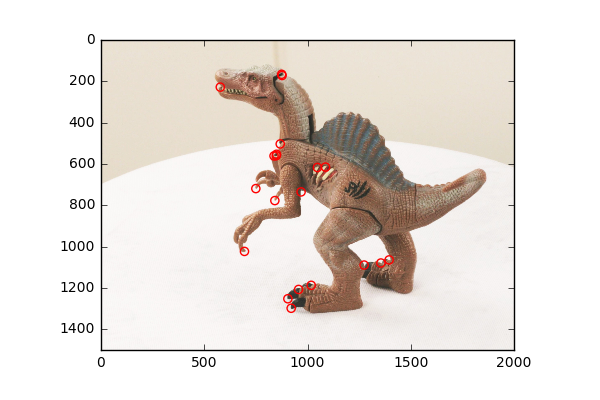
\includegraphics{fig/dinoCorner1.png}
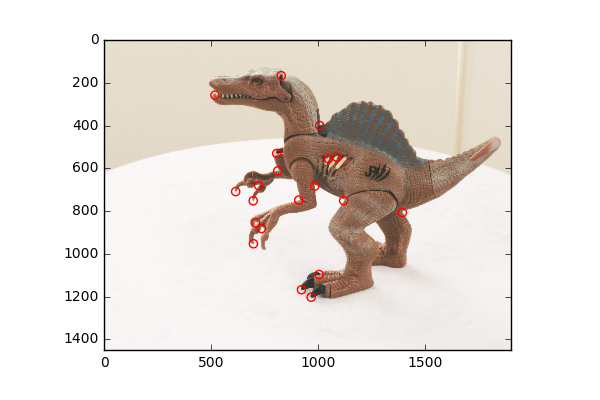
\includegraphics{fig/dinoCorner2.png}

    Comment on your results and observations (3/8 points). You don't need to
comment per output, just \textbf{discuss} any trends you see for the
detected corners as you change the windowSize and increase the smoothing
w.r.t the two pair of images warrior and matrix. Also discuss if you are
able to find corresponding corners for same pair of images.

    \begin{tcolorbox}[breakable, size=fbox, boxrule=1pt, pad at break*=1mm,colback=cellbackground, colframe=cellborder]
\prompt{In}{incolor}{164}{\boxspacing}
\begin{Verbatim}[commandchars=\\\{\}]
\PY{k+kn}{import} \PY{n+nn}{numpy} \PY{k}{as} \PY{n+nn}{np}
\PY{c+c1}{\PYZsh{} from scipy.misc import imread}
\PY{k+kn}{import} \PY{n+nn}{matplotlib}\PY{n+nn}{.}\PY{n+nn}{pyplot} \PY{k}{as} \PY{n+nn}{plt}
\PY{k+kn}{from} \PY{n+nn}{scipy}\PY{n+nn}{.}\PY{n+nn}{ndimage}\PY{n+nn}{.}\PY{n+nn}{filters} \PY{k}{import} \PY{n}{gaussian\PYZus{}filter}
\PY{k+kn}{import} \PY{n+nn}{imageio}
\PY{k+kn}{from} \PY{n+nn}{scipy}\PY{n+nn}{.}\PY{n+nn}{signal} \PY{k}{import} \PY{n}{convolve}
\end{Verbatim}
\end{tcolorbox}

    \begin{tcolorbox}[breakable, size=fbox, boxrule=1pt, pad at break*=1mm,colback=cellbackground, colframe=cellborder]
\prompt{In}{incolor}{165}{\boxspacing}
\begin{Verbatim}[commandchars=\\\{\}]
\PY{k}{def} \PY{n+nf}{rgb2gray}\PY{p}{(}\PY{n}{rgb}\PY{p}{)}\PY{p}{:}
    \PY{l+s+sd}{\PYZdq{}\PYZdq{}\PYZdq{} Convert rgb image to grayscale.}
\PY{l+s+sd}{    \PYZdq{}\PYZdq{}\PYZdq{}}
    \PY{k}{return} \PY{n}{np}\PY{o}{.}\PY{n}{dot}\PY{p}{(}\PY{n}{rgb}\PY{p}{[}\PY{o}{.}\PY{o}{.}\PY{o}{.}\PY{p}{,}\PY{p}{:}\PY{l+m+mi}{3}\PY{p}{]}\PY{p}{,} \PY{p}{[}\PY{l+m+mf}{0.299}\PY{p}{,} \PY{l+m+mf}{0.587}\PY{p}{,} \PY{l+m+mf}{0.114}\PY{p}{]}\PY{p}{)}
\end{Verbatim}
\end{tcolorbox}

    \begin{tcolorbox}[breakable, size=fbox, boxrule=1pt, pad at break*=1mm,colback=cellbackground, colframe=cellborder]
\prompt{In}{incolor}{166}{\boxspacing}
\begin{Verbatim}[commandchars=\\\{\}]
\PY{k}{def} \PY{n+nf}{corner\PYZus{}detect}\PY{p}{(}\PY{n}{image}\PY{p}{,} \PY{n}{nCorners}\PY{p}{,} \PY{n}{smoothSTD}\PY{p}{,} \PY{n}{windowSize}\PY{p}{)}\PY{p}{:}
    \PY{l+s+sd}{\PYZdq{}\PYZdq{}\PYZdq{}Detect corners on a given image.}

\PY{l+s+sd}{    Args:}
\PY{l+s+sd}{        image: Given a grayscale image on which to detect corners.}
\PY{l+s+sd}{        nCorners: Total number of corners to be extracted.}
\PY{l+s+sd}{        smoothSTD: Standard deviation of the Gaussian smoothing kernel.}
\PY{l+s+sd}{        windowSize: Window size for corner detector and non maximum suppression.}

\PY{l+s+sd}{    Returns:}
\PY{l+s+sd}{        Detected corners (in image coordinate) in a numpy array (n*2).}

\PY{l+s+sd}{    \PYZdq{}\PYZdq{}\PYZdq{}}
    
    \PY{l+s+sd}{\PYZdq{}\PYZdq{}\PYZdq{}}
\PY{l+s+sd}{    Put your awesome numpy powered code here:}
\PY{l+s+sd}{    \PYZdq{}\PYZdq{}\PYZdq{}}
    
    \PY{n}{smoothed\PYZus{}image} \PY{o}{=} \PY{n}{gaussian\PYZus{}filter}\PY{p}{(}\PY{n}{image}\PY{p}{,} \PY{n}{smoothSTD}\PY{p}{)}
    \PY{n}{gradient} \PY{o}{=} \PY{n}{np}\PY{o}{.}\PY{n}{array}\PY{p}{(}\PY{p}{[}\PY{o}{\PYZhy{}}\PY{l+m+mf}{0.5}\PY{p}{,} \PY{l+m+mi}{0}\PY{p}{,} \PY{l+m+mf}{0.5}\PY{p}{]}\PY{p}{)}
    
    
    \PY{n}{eig\PYZus{}coordinates} \PY{o}{=} \PY{n+nb}{dict}\PY{p}{(}\PY{p}{)}
    
    \PY{k}{for} \PY{n}{row} \PY{o+ow}{in} \PY{n+nb}{range}\PY{p}{(}\PY{n+nb}{int}\PY{p}{(}\PY{n}{image}\PY{o}{.}\PY{n}{shape}\PY{p}{[}\PY{l+m+mi}{0}\PY{p}{]}\PY{o}{/}\PY{n}{windowSize}\PY{p}{)}\PY{o}{\PYZhy{}}\PY{l+m+mi}{1}\PY{p}{)}\PY{p}{:} \PY{c+c1}{\PYZsh{}scanning with windows}
        \PY{k}{for} \PY{n}{col} \PY{o+ow}{in} \PY{n+nb}{range}\PY{p}{(}\PY{n+nb}{int}\PY{p}{(}\PY{n}{image}\PY{o}{.}\PY{n}{shape}\PY{p}{[}\PY{l+m+mi}{1}\PY{p}{]}\PY{o}{/}\PY{n}{windowSize}\PY{p}{)}\PY{p}{)}\PY{p}{:}
            \PY{n}{block} \PY{o}{=} \PY{n}{image}\PY{p}{[}\PY{n}{windowSize}\PY{o}{*}\PY{n}{row}\PY{p}{:}\PY{n}{windowSize}\PY{o}{*}\PY{n}{row} \PY{o}{+} \PY{n}{windowSize}\PY{p}{,}\PY{n}{windowSize}\PY{o}{*}\PY{n}{col}\PY{p}{:}\PY{n}{windowSize}\PY{o}{*}\PY{n}{col} \PY{o}{+} \PY{n}{windowSize}\PY{p}{]}

            \PY{n}{block\PYZus{}x\PYZus{}ravel} \PY{o}{=} \PY{n}{np}\PY{o}{.}\PY{n}{ravel}\PY{p}{(}\PY{n}{block}\PY{p}{)}
            \PY{n}{block\PYZus{}y\PYZus{}ravel} \PY{o}{=} \PY{n}{np}\PY{o}{.}\PY{n}{ravel}\PY{p}{(}\PY{n}{block}\PY{p}{,} \PY{n}{order}\PY{o}{=}\PY{l+s+s1}{\PYZsq{}}\PY{l+s+s1}{F}\PY{l+s+s1}{\PYZsq{}}\PY{p}{)}
            
            \PY{n}{dx\PYZus{}block} \PY{o}{=} \PY{n}{np}\PY{o}{.}\PY{n}{convolve}\PY{p}{(}\PY{n}{block\PYZus{}x\PYZus{}ravel}\PY{p}{,}\PY{n}{gradient}\PY{p}{)}

            \PY{n}{dy\PYZus{}block} \PY{o}{=} \PY{n}{np}\PY{o}{.}\PY{n}{convolve}\PY{p}{(}\PY{n}{block\PYZus{}y\PYZus{}ravel}\PY{p}{,}\PY{n}{gradient}\PY{p}{)}
            
            \PY{n}{C} \PY{o}{=} \PY{n}{np}\PY{o}{.}\PY{n}{zeros}\PY{p}{(}\PY{p}{(}\PY{l+m+mi}{2}\PY{p}{,}\PY{l+m+mi}{2}\PY{p}{)}\PY{p}{)}
            \PY{n}{C}\PY{p}{[}\PY{l+m+mi}{0}\PY{p}{,}\PY{l+m+mi}{0}\PY{p}{]} \PY{o}{=} \PY{n}{C}\PY{p}{[}\PY{l+m+mi}{0}\PY{p}{,}\PY{l+m+mi}{0}\PY{p}{]} \PY{o}{+} \PY{n}{np}\PY{o}{.}\PY{n}{sum}\PY{p}{(}\PY{n}{np}\PY{o}{.}\PY{n}{square}\PY{p}{(}\PY{n}{dx\PYZus{}block}\PY{p}{)}\PY{p}{)}
            \PY{n}{C}\PY{p}{[}\PY{l+m+mi}{0}\PY{p}{,}\PY{l+m+mi}{1}\PY{p}{]} \PY{o}{=} \PY{n}{C}\PY{p}{[}\PY{l+m+mi}{0}\PY{p}{,}\PY{l+m+mi}{1}\PY{p}{]} \PY{o}{+} \PY{n}{np}\PY{o}{.}\PY{n}{sum}\PY{p}{(}\PY{n}{np}\PY{o}{.}\PY{n}{multiply}\PY{p}{(}\PY{n}{dx\PYZus{}block}\PY{p}{,}\PY{n}{dy\PYZus{}block}\PY{p}{)}\PY{p}{)}
            \PY{n}{C}\PY{p}{[}\PY{l+m+mi}{1}\PY{p}{,}\PY{l+m+mi}{0}\PY{p}{]} \PY{o}{=} \PY{n}{C}\PY{p}{[}\PY{l+m+mi}{0}\PY{p}{,}\PY{l+m+mi}{1}\PY{p}{]} 
            \PY{n}{C}\PY{p}{[}\PY{l+m+mi}{1}\PY{p}{,}\PY{l+m+mi}{1}\PY{p}{]} \PY{o}{=} \PY{n}{C}\PY{p}{[}\PY{l+m+mi}{1}\PY{p}{,}\PY{l+m+mi}{1}\PY{p}{]} \PY{o}{+} \PY{n}{np}\PY{o}{.}\PY{n}{sum}\PY{p}{(}\PY{n}{np}\PY{o}{.}\PY{n}{square}\PY{p}{(}\PY{n}{dy\PYZus{}block}\PY{p}{)}\PY{p}{)}
            \PY{n}{eigenvalues} \PY{o}{=} \PY{n}{np}\PY{o}{.}\PY{n}{linalg}\PY{o}{.}\PY{n}{eigvals}\PY{p}{(}\PY{n}{C}\PY{p}{)}
            \PY{n}{x\PYZus{}pixel} \PY{o}{=} \PY{n}{col}\PY{o}{*}\PY{n}{windowSize} \PY{o}{+} \PY{n}{windowSize}\PY{o}{/}\PY{l+m+mi}{2}
            \PY{n}{y\PYZus{}pixel} \PY{o}{=} \PY{n}{row}\PY{o}{*}\PY{n}{windowSize} \PY{o}{+} \PY{n}{windowSize}\PY{o}{/}\PY{l+m+mi}{2}
            \PY{n}{eig\PYZus{}coordinates}\PY{p}{[}\PY{n+nb}{min}\PY{p}{(}\PY{n}{eigenvalues}\PY{p}{)}\PY{p}{]} \PY{o}{=} \PY{p}{[}\PY{n}{x\PYZus{}pixel}\PY{p}{,}\PY{n}{y\PYZus{}pixel}\PY{p}{]}
    
    \PY{n}{corners} \PY{o}{=} \PY{n}{np}\PY{o}{.}\PY{n}{zeros}\PY{p}{(}\PY{p}{(}\PY{n}{nCorners}\PY{p}{,}\PY{l+m+mi}{2}\PY{p}{)}\PY{p}{)}
    \PY{n}{counter} \PY{o}{=} \PY{l+m+mi}{0}
    \PY{n}{eig\PYZus{}keys} \PY{o}{=} \PY{n+nb}{list}\PY{p}{(}\PY{n}{eig\PYZus{}coordinates}\PY{o}{.}\PY{n}{keys}\PY{p}{(}\PY{p}{)}\PY{p}{)}
    \PY{n}{max\PYZus{}vals} \PY{o}{=} \PY{n+nb}{dict}\PY{p}{(}\PY{p}{)}
    \PY{k}{for} \PY{n}{i} \PY{o+ow}{in} \PY{n+nb}{range}\PY{p}{(}\PY{l+m+mi}{1}\PY{p}{,}\PY{n+nb}{len}\PY{p}{(}\PY{n}{eig\PYZus{}keys}\PY{p}{)}\PY{o}{\PYZhy{}}\PY{l+m+mi}{1}\PY{p}{)}\PY{p}{:}
        \PY{k}{if}\PY{p}{(}\PY{n}{eig\PYZus{}keys}\PY{p}{[}\PY{n}{i}\PY{p}{]} \PY{o}{\PYZgt{}} \PY{n}{eig\PYZus{}keys}\PY{p}{[}\PY{n}{i}\PY{o}{\PYZhy{}}\PY{l+m+mi}{1}\PY{p}{]} \PY{o+ow}{and} \PY{n}{eig\PYZus{}keys}\PY{p}{[}\PY{n}{i}\PY{p}{]} \PY{o}{\PYZgt{}} \PY{n}{eig\PYZus{}keys}\PY{p}{[}\PY{n}{i}\PY{o}{+}\PY{l+m+mi}{1}\PY{p}{]}\PY{p}{)}\PY{p}{:} \PY{c+c1}{\PYZsh{}Finding local maximums}
            \PY{n}{max\PYZus{}vals}\PY{p}{[}\PY{n}{eig\PYZus{}keys}\PY{p}{[}\PY{n}{i}\PY{p}{]}\PY{p}{]} \PY{o}{=} \PY{n}{eig\PYZus{}coordinates}\PY{p}{[}\PY{n}{eig\PYZus{}keys}\PY{p}{[}\PY{n}{i}\PY{p}{]}\PY{p}{]}                 
            
    \PY{n}{sorted\PYZus{}max\PYZus{}val\PYZus{}keys} \PY{o}{=} \PY{n+nb}{sorted}\PY{p}{(}\PY{n}{max\PYZus{}vals}\PY{o}{.}\PY{n}{keys}\PY{p}{(}\PY{p}{)}\PY{p}{,} \PY{n}{reverse}\PY{o}{=}\PY{k+kc}{True}\PY{p}{)}\PY{c+c1}{\PYZsh{}sorting in descending order  }
    \PY{k}{for} \PY{n}{i} \PY{o+ow}{in} \PY{n+nb}{range}\PY{p}{(}\PY{n}{nCorners}\PY{p}{)}\PY{p}{:} \PY{c+c1}{\PYZsh{}selecting top corners}
        \PY{n}{xy\PYZus{}coords} \PY{o}{=} \PY{n}{max\PYZus{}vals}\PY{p}{[}\PY{n}{sorted\PYZus{}max\PYZus{}val\PYZus{}keys}\PY{p}{[}\PY{n}{i}\PY{p}{]}\PY{p}{]}
        \PY{n}{corners}\PY{p}{[}\PY{n}{i}\PY{p}{,}\PY{l+m+mi}{0}\PY{p}{]} \PY{o}{=} \PY{n}{xy\PYZus{}coords}\PY{p}{[}\PY{l+m+mi}{0}\PY{p}{]} 
        \PY{n}{corners}\PY{p}{[}\PY{n}{i}\PY{p}{,}\PY{l+m+mi}{1}\PY{p}{]} \PY{o}{=} \PY{n}{xy\PYZus{}coords}\PY{p}{[}\PY{l+m+mi}{1}\PY{p}{]}
    
    \PY{k}{return} \PY{n}{corners}
\end{Verbatim}
\end{tcolorbox}

    \begin{tcolorbox}[breakable, size=fbox, boxrule=1pt, pad at break*=1mm,colback=cellbackground, colframe=cellborder]
\prompt{In}{incolor}{167}{\boxspacing}
\begin{Verbatim}[commandchars=\\\{\}]
\PY{k}{def} \PY{n+nf}{show\PYZus{}corners\PYZus{}result}\PY{p}{(}\PY{n}{imgs}\PY{p}{,} \PY{n}{corners}\PY{p}{)}\PY{p}{:}
    \PY{n}{fig} \PY{o}{=} \PY{n}{plt}\PY{o}{.}\PY{n}{figure}\PY{p}{(}\PY{n}{figsize}\PY{o}{=}\PY{p}{(}\PY{l+m+mi}{15}\PY{p}{,} \PY{l+m+mi}{15}\PY{p}{)}\PY{p}{)}
    \PY{n}{ax1} \PY{o}{=} \PY{n}{fig}\PY{o}{.}\PY{n}{add\PYZus{}subplot}\PY{p}{(}\PY{l+m+mi}{221}\PY{p}{)}
    \PY{n}{ax1}\PY{o}{.}\PY{n}{imshow}\PY{p}{(}\PY{n}{imgs}\PY{p}{[}\PY{l+m+mi}{0}\PY{p}{]}\PY{p}{,} \PY{n}{cmap}\PY{o}{=}\PY{l+s+s1}{\PYZsq{}}\PY{l+s+s1}{gray}\PY{l+s+s1}{\PYZsq{}}\PY{p}{)}
    \PY{n}{ax1}\PY{o}{.}\PY{n}{scatter}\PY{p}{(}\PY{n}{corners}\PY{p}{[}\PY{l+m+mi}{0}\PY{p}{]}\PY{p}{[}\PY{p}{:}\PY{p}{,} \PY{l+m+mi}{0}\PY{p}{]}\PY{p}{,} \PY{n}{corners}\PY{p}{[}\PY{l+m+mi}{0}\PY{p}{]}\PY{p}{[}\PY{p}{:}\PY{p}{,} \PY{l+m+mi}{1}\PY{p}{]}\PY{p}{,} \PY{n}{s}\PY{o}{=}\PY{l+m+mi}{36}\PY{p}{,} \PY{n}{edgecolors}\PY{o}{=}\PY{l+s+s1}{\PYZsq{}}\PY{l+s+s1}{r}\PY{l+s+s1}{\PYZsq{}}\PY{p}{,} \PY{n}{facecolors}\PY{o}{=}\PY{l+s+s1}{\PYZsq{}}\PY{l+s+s1}{none}\PY{l+s+s1}{\PYZsq{}}\PY{p}{)}

    \PY{n}{ax2} \PY{o}{=} \PY{n}{fig}\PY{o}{.}\PY{n}{add\PYZus{}subplot}\PY{p}{(}\PY{l+m+mi}{222}\PY{p}{)}
    \PY{n}{ax2}\PY{o}{.}\PY{n}{imshow}\PY{p}{(}\PY{n}{imgs}\PY{p}{[}\PY{l+m+mi}{1}\PY{p}{]}\PY{p}{,} \PY{n}{cmap}\PY{o}{=}\PY{l+s+s1}{\PYZsq{}}\PY{l+s+s1}{gray}\PY{l+s+s1}{\PYZsq{}}\PY{p}{)}
    \PY{n}{ax2}\PY{o}{.}\PY{n}{scatter}\PY{p}{(}\PY{n}{corners}\PY{p}{[}\PY{l+m+mi}{1}\PY{p}{]}\PY{p}{[}\PY{p}{:}\PY{p}{,} \PY{l+m+mi}{0}\PY{p}{]}\PY{p}{,} \PY{n}{corners}\PY{p}{[}\PY{l+m+mi}{1}\PY{p}{]}\PY{p}{[}\PY{p}{:}\PY{p}{,} \PY{l+m+mi}{1}\PY{p}{]}\PY{p}{,} \PY{n}{s}\PY{o}{=}\PY{l+m+mi}{36}\PY{p}{,} \PY{n}{edgecolors}\PY{o}{=}\PY{l+s+s1}{\PYZsq{}}\PY{l+s+s1}{r}\PY{l+s+s1}{\PYZsq{}}\PY{p}{,} \PY{n}{facecolors}\PY{o}{=}\PY{l+s+s1}{\PYZsq{}}\PY{l+s+s1}{none}\PY{l+s+s1}{\PYZsq{}}\PY{p}{)}
    \PY{n}{plt}\PY{o}{.}\PY{n}{show}\PY{p}{(}\PY{p}{)}
\end{Verbatim}
\end{tcolorbox}

    \begin{tcolorbox}[breakable, size=fbox, boxrule=1pt, pad at break*=1mm,colback=cellbackground, colframe=cellborder]
\prompt{In}{incolor}{168}{\boxspacing}
\begin{Verbatim}[commandchars=\\\{\}]
\PY{c+c1}{\PYZsh{} detect corners on warrior and matrix image sets}
\PY{c+c1}{\PYZsh{} adjust your corner detection parameters here}
\PY{n}{nCorners} \PY{o}{=} \PY{l+m+mi}{20}
\PY{n}{smoothSTDs} \PY{o}{=} \PY{p}{[}\PY{l+m+mf}{0.5}\PY{p}{,} \PY{l+m+mi}{1}\PY{p}{,} \PY{l+m+mi}{2}\PY{p}{,} \PY{l+m+mi}{4}\PY{p}{]}
\PY{n}{imgs\PYZus{}mat} \PY{o}{=} \PY{p}{[}\PY{p}{]}
\PY{n}{imgs\PYZus{}war} \PY{o}{=} \PY{p}{[}\PY{p}{]}
\PY{n}{imgs\PYZus{}dino} \PY{o}{=} \PY{p}{[}\PY{p}{]}
\PY{n}{grayimgs\PYZus{}mat} \PY{o}{=} \PY{p}{[}\PY{p}{]}
\PY{n}{grayimgs\PYZus{}war} \PY{o}{=} \PY{p}{[}\PY{p}{]}
\PY{n}{grayimgs\PYZus{}dino} \PY{o}{=} \PY{p}{[}\PY{p}{]}
\PY{c+c1}{\PYZsh{} Read the two images and convert it to Greyscale}
\PY{k}{for} \PY{n}{i} \PY{o+ow}{in} \PY{n+nb}{range}\PY{p}{(}\PY{l+m+mi}{2}\PY{p}{)}\PY{p}{:}
    \PY{n}{img\PYZus{}mat} \PY{o}{=} \PY{n}{imageio}\PY{o}{.}\PY{n}{imread}\PY{p}{(}\PY{l+s+s1}{\PYZsq{}}\PY{l+s+s1}{p4/matrix/matrix}\PY{l+s+s1}{\PYZsq{}} \PY{o}{+} \PY{n+nb}{str}\PY{p}{(}\PY{n}{i}\PY{p}{)} \PY{o}{+} \PY{l+s+s1}{\PYZsq{}}\PY{l+s+s1}{.png}\PY{l+s+s1}{\PYZsq{}}\PY{p}{)}
    \PY{n}{imgs\PYZus{}mat}\PY{o}{.}\PY{n}{append}\PY{p}{(}\PY{n}{img\PYZus{}mat}\PY{p}{)} 
    \PY{n}{grayimgs\PYZus{}mat}\PY{o}{.}\PY{n}{append}\PY{p}{(}\PY{n}{rgb2gray}\PY{p}{(}\PY{n}{img\PYZus{}mat}\PY{p}{)}\PY{p}{)}
    \PY{c+c1}{\PYZsh{} Comment above line and uncomment below line to}
    \PY{c+c1}{\PYZsh{} downsize your image in case corner\PYZus{}detect runs slow in test }
    \PY{c+c1}{\PYZsh{}grayimgs\PYZus{}mat.append(rgb2gray(img\PYZus{}mat)[::2, ::2])}
    \PY{c+c1}{\PYZsh{} if you unleash the power of numpy you wouldn\PYZsq{}t need to downsize, it\PYZsq{}ll be fast}
    \PY{n}{img\PYZus{}war} \PY{o}{=} \PY{n}{imageio}\PY{o}{.}\PY{n}{imread}\PY{p}{(}\PY{l+s+s1}{\PYZsq{}}\PY{l+s+s1}{p4/warrior/warrior}\PY{l+s+s1}{\PYZsq{}} \PY{o}{+} \PY{n+nb}{str}\PY{p}{(}\PY{n}{i}\PY{p}{)} \PY{o}{+} \PY{l+s+s1}{\PYZsq{}}\PY{l+s+s1}{.png}\PY{l+s+s1}{\PYZsq{}}\PY{p}{)}
    \PY{n}{imgs\PYZus{}war}\PY{o}{.}\PY{n}{append}\PY{p}{(}\PY{n}{img\PYZus{}war}\PY{p}{)}
    \PY{n}{grayimgs\PYZus{}war}\PY{o}{.}\PY{n}{append}\PY{p}{(}\PY{n}{rgb2gray}\PY{p}{(}\PY{n}{img\PYZus{}war}\PY{p}{)}\PY{p}{)}
    \PY{n}{img\PYZus{}dino} \PY{o}{=} \PY{n}{imageio}\PY{o}{.}\PY{n}{imread}\PY{p}{(}\PY{l+s+s1}{\PYZsq{}}\PY{l+s+s1}{p4/dino/dino}\PY{l+s+s1}{\PYZsq{}} \PY{o}{+} \PY{n+nb}{str}\PY{p}{(}\PY{n}{i}\PY{p}{)} \PY{o}{+} \PY{l+s+s1}{\PYZsq{}}\PY{l+s+s1}{.png}\PY{l+s+s1}{\PYZsq{}}\PY{p}{)}
    \PY{n}{imgs\PYZus{}dino}\PY{o}{.}\PY{n}{append}\PY{p}{(}\PY{n}{img\PYZus{}dino}\PY{p}{)}
    \PY{n}{grayimgs\PYZus{}dino}\PY{o}{.}\PY{n}{append}\PY{p}{(}\PY{n}{rgb2gray}\PY{p}{(}\PY{n}{img\PYZus{}dino}\PY{p}{)}\PY{p}{)}
    
\PY{k}{for} \PY{n}{smoothSTD} \PY{o+ow}{in} \PY{n}{smoothSTDs}\PY{p}{:}
    \PY{n}{windowSize} \PY{o}{=} \PY{n+nb}{int}\PY{p}{(}\PY{l+m+mi}{6}\PY{o}{*}\PY{n}{smoothSTD}\PY{p}{)}
    \PY{k}{if} \PY{n}{windowSize}\PY{o}{\PYZpc{}}\PY{k}{2}==0: windowSize += 1
    \PY{n}{crns\PYZus{}mat} \PY{o}{=} \PY{p}{[}\PY{p}{]}
    \PY{n}{crns\PYZus{}war} \PY{o}{=} \PY{p}{[}\PY{p}{]}
    \PY{n}{crns\PYZus{}dino} \PY{o}{=} \PY{p}{[}\PY{p}{]}
    \PY{n+nb}{print} \PY{p}{(}\PY{l+s+s2}{\PYZdq{}}\PY{l+s+s2}{SmoothSTD:}\PY{l+s+s2}{\PYZdq{}}\PY{p}{,} \PY{n}{smoothSTD}\PY{p}{,} \PY{l+s+s2}{\PYZdq{}}\PY{l+s+s2}{WindowSize:}\PY{l+s+s2}{\PYZdq{}}\PY{p}{,} \PY{n}{windowSize}\PY{p}{)}
    \PY{k}{for} \PY{n}{i} \PY{o+ow}{in} \PY{n+nb}{range}\PY{p}{(}\PY{l+m+mi}{2}\PY{p}{)}\PY{p}{:}
        \PY{n}{crns\PYZus{}mat}\PY{o}{.}\PY{n}{append}\PY{p}{(}\PY{n}{corner\PYZus{}detect}\PY{p}{(}\PY{n}{grayimgs\PYZus{}mat}\PY{p}{[}\PY{n}{i}\PY{p}{]}\PY{p}{,} \PY{n}{nCorners}\PY{p}{,} \PY{n}{smoothSTD}\PY{p}{,}\PYZbs{}
                                      \PY{n}{windowSize}\PY{p}{)}\PY{p}{)}
        \PY{n}{crns\PYZus{}war}\PY{o}{.}\PY{n}{append}\PY{p}{(}\PY{n}{corner\PYZus{}detect}\PY{p}{(}\PY{n}{grayimgs\PYZus{}war}\PY{p}{[}\PY{n}{i}\PY{p}{]}\PY{p}{,} \PY{n}{nCorners}\PY{p}{,} \PY{n}{smoothSTD}\PY{p}{,}\PYZbs{}
                                      \PY{n}{windowSize}\PY{p}{)}\PY{p}{)}
        \PY{n}{crns\PYZus{}dino}\PY{o}{.}\PY{n}{append}\PY{p}{(}\PY{n}{corner\PYZus{}detect}\PY{p}{(}\PY{n}{grayimgs\PYZus{}dino}\PY{p}{[}\PY{n}{i}\PY{p}{]}\PY{p}{,} \PY{n}{nCorners}\PY{p}{,} \PY{n}{smoothSTD}\PY{p}{,}\PYZbs{}
                                      \PY{n}{windowSize}\PY{p}{)}\PY{p}{)}
    \PY{n}{show\PYZus{}corners\PYZus{}result}\PY{p}{(}\PY{n}{imgs\PYZus{}mat}\PY{p}{,} \PY{n}{crns\PYZus{}mat}\PY{p}{)} \PY{c+c1}{\PYZsh{}uncomment this to show your output!}
    \PY{n}{show\PYZus{}corners\PYZus{}result}\PY{p}{(}\PY{n}{imgs\PYZus{}war}\PY{p}{,} \PY{n}{crns\PYZus{}war}\PY{p}{)}
    \PY{c+c1}{\PYZsh{}show\PYZus{}corners\PYZus{}result(imgs\PYZus{}dino, crns\PYZus{}dino)}
\end{Verbatim}
\end{tcolorbox}

    \begin{Verbatim}[commandchars=\\\{\}]
SmoothSTD: 0.5 WindowSize: 3
    \end{Verbatim}

    \begin{center}
    \adjustimage{max size={0.9\linewidth}{0.9\paperheight}}{output_13_1.png}
    \end{center}
    { \hspace*{\fill} \\}
    
    \begin{center}
    \adjustimage{max size={0.9\linewidth}{0.9\paperheight}}{output_13_2.png}
    \end{center}
    { \hspace*{\fill} \\}
    
    \begin{Verbatim}[commandchars=\\\{\}]
SmoothSTD: 1 WindowSize: 7
    \end{Verbatim}

    \begin{center}
    \adjustimage{max size={0.9\linewidth}{0.9\paperheight}}{output_13_4.png}
    \end{center}
    { \hspace*{\fill} \\}
    
    \begin{center}
    \adjustimage{max size={0.9\linewidth}{0.9\paperheight}}{output_13_5.png}
    \end{center}
    { \hspace*{\fill} \\}
    
    \begin{Verbatim}[commandchars=\\\{\}]
SmoothSTD: 2 WindowSize: 13
    \end{Verbatim}

    \begin{center}
    \adjustimage{max size={0.9\linewidth}{0.9\paperheight}}{output_13_7.png}
    \end{center}
    { \hspace*{\fill} \\}
    
    \begin{center}
    \adjustimage{max size={0.9\linewidth}{0.9\paperheight}}{output_13_8.png}
    \end{center}
    { \hspace*{\fill} \\}
    
    \begin{Verbatim}[commandchars=\\\{\}]
SmoothSTD: 4 WindowSize: 25
    \end{Verbatim}

    \begin{center}
    \adjustimage{max size={0.9\linewidth}{0.9\paperheight}}{output_13_10.png}
    \end{center}
    { \hspace*{\fill} \\}
    
    \begin{center}
    \adjustimage{max size={0.9\linewidth}{0.9\paperheight}}{output_13_11.png}
    \end{center}
    { \hspace*{\fill} \\}
    
    \[\textbf{Results and Observations}\] When the window size and stdev
(the window size is a function of the stdev) are smaller, there are
clumps of detection circles in the area of a corner. The corner
detection algorithm is more sensitive to the gradient change when the
window size is smaller. I think a good analogy is that a bigger window
is like looking at a mountain from miles away - the mountain looks
smooth and you can clearly see the absolute maximum of the mountain (the
peak). However, when you are actually on the mountain (small window) you
can now see the rugged surface of the mountain and see all these bumps
and ``local maximums''. The larger window is missing these smaller bumps
and doesn't register them as corners, so it does a better job at
locating the ``true'' corners of the image with a single detection
circle.

Corresponding corners on warrior: both ends of the hammer, wrist, part
of the cape, his far side hip, the bottom bit of his front garment

Corresponding corners on Morpheus: ankle, finger, wrist, cape corner
(all on left side of images)

More points correspond between the warrior images and many points for
Morpheous don't correspond as the shift in perspective angle has a big
effect on the corner detection.

    \hypertarget{ncc-normalized-cross-correlation-matching-2-pts}{%
\subsubsection{NCC (Normalized Cross-Correlation) Matching {[}2
pts{]}}\label{ncc-normalized-cross-correlation-matching-2-pts}}

Write a function ncc\_match that implements the NCC matching algorithm
for two input windows. NCC =
\(\sum_{i,j}\tilde{W_1} (i,j)\cdot \tilde{W_2} (i,j)\) where
\(\tilde{W} = \frac{W - \overline{W}}{\sqrt{\sum_{k,l}(W(k,l) - \overline{W})^2}}\)
is a mean-shifted and normalized version of the window and
\(\overline{W}\) is the mean pixel value in the window W.

    \begin{tcolorbox}[breakable, size=fbox, boxrule=1pt, pad at break*=1mm,colback=cellbackground, colframe=cellborder]
\prompt{In}{incolor}{169}{\boxspacing}
\begin{Verbatim}[commandchars=\\\{\}]
\PY{k}{def} \PY{n+nf}{ncc\PYZus{}match}\PY{p}{(}\PY{n}{img1}\PY{p}{,} \PY{n}{img2}\PY{p}{,} \PY{n}{c1}\PY{p}{,} \PY{n}{c2}\PY{p}{,} \PY{n}{R}\PY{p}{)}\PY{p}{:}
    \PY{l+s+sd}{\PYZdq{}\PYZdq{}\PYZdq{}Compute NCC given two windows.}

\PY{l+s+sd}{    Args:}
\PY{l+s+sd}{        img1: Image 1.}
\PY{l+s+sd}{        img2: Image 2.}
\PY{l+s+sd}{        c1: Center (in image coordinate) of the window in image 1.}
\PY{l+s+sd}{        c2: Center (in image coordinate) of the window in image 2.}
\PY{l+s+sd}{        R: R is the radius of the patch, 2 * R + 1 is the window size}

\PY{l+s+sd}{    Returns:}
\PY{l+s+sd}{        NCC matching score for two input windows.}

\PY{l+s+sd}{    \PYZdq{}\PYZdq{}\PYZdq{}}
    
    \PY{l+s+sd}{\PYZdq{}\PYZdq{}\PYZdq{}}
\PY{l+s+sd}{    Your code here:}
\PY{l+s+sd}{    \PYZdq{}\PYZdq{}\PYZdq{}}
    \PY{n}{row\PYZus{}start1} \PY{o}{=} \PY{n+nb}{int}\PY{p}{(}\PY{n}{c1}\PY{p}{[}\PY{l+m+mi}{1}\PY{p}{]}\PY{o}{\PYZhy{}}\PY{n}{R}\PY{p}{)}
    \PY{n}{col\PYZus{}start1} \PY{o}{=} \PY{n+nb}{int}\PY{p}{(}\PY{n}{c1}\PY{p}{[}\PY{l+m+mi}{0}\PY{p}{]}\PY{o}{\PYZhy{}}\PY{n}{R}\PY{p}{)}
    \PY{n}{row\PYZus{}start2} \PY{o}{=} \PY{n+nb}{int}\PY{p}{(}\PY{n}{c2}\PY{p}{[}\PY{l+m+mi}{1}\PY{p}{]}\PY{o}{\PYZhy{}}\PY{n}{R}\PY{p}{)}
    \PY{n}{col\PYZus{}start2} \PY{o}{=} \PY{n+nb}{int}\PY{p}{(}\PY{n}{c2}\PY{p}{[}\PY{l+m+mi}{0}\PY{p}{]}\PY{o}{\PYZhy{}}\PY{n}{R}\PY{p}{)}
    
    \PY{n}{W1} \PY{o}{=} \PY{n}{img1}\PY{p}{[}\PY{n}{row\PYZus{}start1}\PY{p}{:}\PY{n}{row\PYZus{}start1}\PY{o}{+}\PY{l+m+mi}{2}\PY{o}{*}\PY{n}{R}\PY{o}{+}\PY{l+m+mi}{1}\PY{p}{,}\PY{n}{col\PYZus{}start1}\PY{p}{:}\PY{n}{col\PYZus{}start1}\PY{o}{+}\PY{l+m+mi}{2}\PY{o}{*}\PY{n}{R}\PY{o}{+}\PY{l+m+mi}{1}\PY{p}{]}
    \PY{n}{W2} \PY{o}{=} \PY{n}{img2}\PY{p}{[}\PY{n}{row\PYZus{}start2}\PY{p}{:}\PY{n}{row\PYZus{}start2}\PY{o}{+}\PY{l+m+mi}{2}\PY{o}{*}\PY{n}{R}\PY{o}{+}\PY{l+m+mi}{1}\PY{p}{,}\PY{n}{col\PYZus{}start2}\PY{p}{:}\PY{n}{col\PYZus{}start2}\PY{o}{+}\PY{l+m+mi}{2}\PY{o}{*}\PY{n}{R}\PY{o}{+}\PY{l+m+mi}{1}\PY{p}{]}
    
    \PY{n}{W\PYZus{}bar1} \PY{o}{=} \PY{n}{np}\PY{o}{.}\PY{n}{mean}\PY{p}{(}\PY{n}{W1}\PY{p}{)}
    \PY{n}{W\PYZus{}bar2} \PY{o}{=} \PY{n}{np}\PY{o}{.}\PY{n}{mean}\PY{p}{(}\PY{n}{W2}\PY{p}{)}

    \PY{n}{W\PYZus{}tilde1} \PY{o}{=} \PY{p}{(}\PY{n}{np}\PY{o}{.}\PY{n}{subtract}\PY{p}{(}\PY{n}{W1}\PY{p}{,} \PY{n}{W\PYZus{}bar1}\PY{p}{)}\PY{p}{)}\PY{o}{/}\PY{n}{np}\PY{o}{.}\PY{n}{sqrt}\PY{p}{(}\PY{n}{np}\PY{o}{.}\PY{n}{sum}\PY{p}{(}\PY{n}{np}\PY{o}{.}\PY{n}{square}\PY{p}{(}\PY{n}{np}\PY{o}{.}\PY{n}{subtract}\PY{p}{(}\PY{n}{W1}\PY{p}{,}\PY{n}{W\PYZus{}bar1}\PY{p}{)}\PY{p}{)}\PY{p}{)}\PY{p}{)}
    \PY{n}{W\PYZus{}tilde2} \PY{o}{=} \PY{p}{(}\PY{n}{np}\PY{o}{.}\PY{n}{subtract}\PY{p}{(}\PY{n}{W2}\PY{p}{,} \PY{n}{W\PYZus{}bar2}\PY{p}{)}\PY{p}{)}\PY{o}{/}\PY{n}{np}\PY{o}{.}\PY{n}{sqrt}\PY{p}{(}\PY{n}{np}\PY{o}{.}\PY{n}{sum}\PY{p}{(}\PY{n}{np}\PY{o}{.}\PY{n}{square}\PY{p}{(}\PY{n}{np}\PY{o}{.}\PY{n}{subtract}\PY{p}{(}\PY{n}{W2}\PY{p}{,}\PY{n}{W\PYZus{}bar2}\PY{p}{)}\PY{p}{)}\PY{p}{)}\PY{p}{)}
    \PY{n}{matching\PYZus{}score} \PY{o}{=} \PY{l+m+mi}{0}
    \PY{k}{try}\PY{p}{:}
        \PY{n}{matching\PYZus{}score} \PY{o}{=} \PY{n}{np}\PY{o}{.}\PY{n}{sum}\PY{p}{(}\PY{n}{np}\PY{o}{.}\PY{n}{multiply}\PY{p}{(}\PY{n}{W\PYZus{}tilde1}\PY{p}{,} \PY{n}{W\PYZus{}tilde2}\PY{p}{)}\PY{p}{)}
    \PY{k}{except} \PY{n+ne}{ValueError}\PY{p}{:}
        \PY{n}{matching\PYZus{}score} \PY{o}{=} \PY{n}{matching\PYZus{}score}
    \PY{k}{return} \PY{n}{matching\PYZus{}score}
\end{Verbatim}
\end{tcolorbox}

    \begin{tcolorbox}[breakable, size=fbox, boxrule=1pt, pad at break*=1mm,colback=cellbackground, colframe=cellborder]
\prompt{In}{incolor}{170}{\boxspacing}
\begin{Verbatim}[commandchars=\\\{\}]
\PY{c+c1}{\PYZsh{} test NCC match}
\PY{n}{img1} \PY{o}{=} \PY{n}{np}\PY{o}{.}\PY{n}{array}\PY{p}{(}\PY{p}{[}\PY{p}{[}\PY{l+m+mi}{1}\PY{p}{,} \PY{l+m+mi}{2}\PY{p}{,} \PY{l+m+mi}{3}\PY{p}{,} \PY{l+m+mi}{4}\PY{p}{]}\PY{p}{,} \PY{p}{[}\PY{l+m+mi}{4}\PY{p}{,} \PY{l+m+mi}{5}\PY{p}{,} \PY{l+m+mi}{6}\PY{p}{,} \PY{l+m+mi}{8}\PY{p}{]}\PY{p}{,} \PY{p}{[}\PY{l+m+mi}{7}\PY{p}{,} \PY{l+m+mi}{8}\PY{p}{,} \PY{l+m+mi}{9}\PY{p}{,} \PY{l+m+mi}{4}\PY{p}{]}\PY{p}{]}\PY{p}{)}
\PY{n}{img2} \PY{o}{=} \PY{n}{np}\PY{o}{.}\PY{n}{array}\PY{p}{(}\PY{p}{[}\PY{p}{[}\PY{l+m+mi}{1}\PY{p}{,} \PY{l+m+mi}{2}\PY{p}{,} \PY{l+m+mi}{1}\PY{p}{,} \PY{l+m+mi}{3}\PY{p}{]}\PY{p}{,} \PY{p}{[}\PY{l+m+mi}{6}\PY{p}{,} \PY{l+m+mi}{5}\PY{p}{,} \PY{l+m+mi}{4}\PY{p}{,} \PY{l+m+mi}{4}\PY{p}{]}\PY{p}{,} \PY{p}{[}\PY{l+m+mi}{9}\PY{p}{,} \PY{l+m+mi}{8}\PY{p}{,} \PY{l+m+mi}{7}\PY{p}{,} \PY{l+m+mi}{3}\PY{p}{]}\PY{p}{]}\PY{p}{)}
\PY{n+nb}{print} \PY{p}{(}\PY{n}{ncc\PYZus{}match}\PY{p}{(}\PY{n}{img1}\PY{p}{,} \PY{n}{img2}\PY{p}{,} \PY{n}{np}\PY{o}{.}\PY{n}{array}\PY{p}{(}\PY{p}{[}\PY{l+m+mi}{1}\PY{p}{,} \PY{l+m+mi}{1}\PY{p}{]}\PY{p}{)}\PY{p}{,} \PY{n}{np}\PY{o}{.}\PY{n}{array}\PY{p}{(}\PY{p}{[}\PY{l+m+mi}{1}\PY{p}{,} \PY{l+m+mi}{1}\PY{p}{]}\PY{p}{)}\PY{p}{,} \PY{l+m+mi}{1}\PY{p}{)}\PY{p}{)}
\PY{c+c1}{\PYZsh{} should print 0.8546}
\PY{n+nb}{print} \PY{p}{(}\PY{n}{ncc\PYZus{}match}\PY{p}{(}\PY{n}{img1}\PY{p}{,} \PY{n}{img2}\PY{p}{,} \PY{n}{np}\PY{o}{.}\PY{n}{array}\PY{p}{(}\PY{p}{[}\PY{l+m+mi}{2}\PY{p}{,} \PY{l+m+mi}{1}\PY{p}{]}\PY{p}{)}\PY{p}{,} \PY{n}{np}\PY{o}{.}\PY{n}{array}\PY{p}{(}\PY{p}{[}\PY{l+m+mi}{2}\PY{p}{,} \PY{l+m+mi}{1}\PY{p}{]}\PY{p}{)}\PY{p}{,} \PY{l+m+mi}{1}\PY{p}{)}\PY{p}{)}
\PY{c+c1}{\PYZsh{} should print 0.8457}
\PY{n+nb}{print} \PY{p}{(}\PY{n}{ncc\PYZus{}match}\PY{p}{(}\PY{n}{img1}\PY{p}{,} \PY{n}{img2}\PY{p}{,} \PY{n}{np}\PY{o}{.}\PY{n}{array}\PY{p}{(}\PY{p}{[}\PY{l+m+mi}{1}\PY{p}{,} \PY{l+m+mi}{1}\PY{p}{]}\PY{p}{)}\PY{p}{,} \PY{n}{np}\PY{o}{.}\PY{n}{array}\PY{p}{(}\PY{p}{[}\PY{l+m+mi}{2}\PY{p}{,} \PY{l+m+mi}{1}\PY{p}{]}\PY{p}{)}\PY{p}{,} \PY{l+m+mi}{1}\PY{p}{)}\PY{p}{)}
\PY{c+c1}{\PYZsh{} should print 0.6258}
\end{Verbatim}
\end{tcolorbox}

    \begin{Verbatim}[commandchars=\\\{\}]
0.8546547739343037
0.8457615282174419
0.6258689611426174
    \end{Verbatim}

    \hypertarget{naive-matching-4-pts}{%
\subsubsection{Naive Matching {[}4 pts{]}}\label{naive-matching-4-pts}}

Equipped with the corner detector and the NCC matching function, we are
ready to start finding correspondances. One naive strategy is to try and
find the best match between the two sets of corner points. Write a
script that does this, namely, for each corner in image1, find the best
match from the detected corners in image2 (or, if the NCC match score is
too low, then return no match for that point). You will have to figure
out a good threshold (NCCth) value by experimentation. Write a function
naive\_matching and call it as below. Examine your results for 10, 20,
and 30 detected corners in each image. Choose number of detected corners
to maximize the number of correct matching pairs. naive\_matching will
call your NCC matching code. \textbf{Properly label or mention which
output corresponds to which choice of number of corners. Total number of
output is 6 images} (3 choice of number of corners for each matrix and
warrior), where one image is like below:

Number of Corners: 10 

    \begin{tcolorbox}[breakable, size=fbox, boxrule=1pt, pad at break*=1mm,colback=cellbackground, colframe=cellborder]
\prompt{In}{incolor}{171}{\boxspacing}
\begin{Verbatim}[commandchars=\\\{\}]
\PY{k}{def} \PY{n+nf}{naive\PYZus{}matching}\PY{p}{(}\PY{n}{img1}\PY{p}{,} \PY{n}{img2}\PY{p}{,} \PY{n}{corners1}\PY{p}{,} \PY{n}{corners2}\PY{p}{,} \PY{n}{R}\PY{p}{,} \PY{n}{NCCth}\PY{p}{)}\PY{p}{:}
    \PY{l+s+sd}{\PYZdq{}\PYZdq{}\PYZdq{}Compute NCC given two windows.}

\PY{l+s+sd}{    Args:}
\PY{l+s+sd}{        img1: Image 1.}
\PY{l+s+sd}{        img2: Image 2.}
\PY{l+s+sd}{        corners1: Corners in image 1 (nx2)}
\PY{l+s+sd}{        corners2: Corners in image 2 (nx2)}
\PY{l+s+sd}{        R: NCC matching radius}
\PY{l+s+sd}{        NCCth: NCC matching score threshold}

\PY{l+s+sd}{    Returns:}
\PY{l+s+sd}{        NCC matching result a list of tuple (c1, c2), }
\PY{l+s+sd}{        c1 is the 1x2 corner location in image 1, }
\PY{l+s+sd}{        c2 is the 1x2 corner location in image 2. }

\PY{l+s+sd}{    \PYZdq{}\PYZdq{}\PYZdq{}}
    
    \PY{l+s+sd}{\PYZdq{}\PYZdq{}\PYZdq{}}
\PY{l+s+sd}{    Your code here:}
\PY{l+s+sd}{    \PYZdq{}\PYZdq{}\PYZdq{}}
    \PY{n}{matching} \PY{o}{=} \PY{p}{[}\PY{p}{]}
    \PY{n}{distance\PYZus{}ratio\PYZus{}threshold} \PY{o}{=} \PY{l+m+mf}{0.8}
    \PY{n}{already\PYZus{}matched}\PY{o}{=}\PY{p}{[}\PY{p}{]}
    \PY{k}{for} \PY{n}{i} \PY{o+ow}{in} \PY{n+nb}{range}\PY{p}{(}\PY{n}{corners1}\PY{o}{.}\PY{n}{shape}\PY{p}{[}\PY{l+m+mi}{0}\PY{p}{]}\PY{p}{)}\PY{p}{:}
        \PY{n}{NCCth\PYZus{}dict} \PY{o}{=} \PY{n+nb}{dict}\PY{p}{(}\PY{p}{)}
        \PY{k}{for} \PY{n}{j} \PY{o+ow}{in} \PY{n+nb}{range}\PY{p}{(}\PY{n}{corners2}\PY{o}{.}\PY{n}{shape}\PY{p}{[}\PY{l+m+mi}{0}\PY{p}{]}\PY{p}{)}\PY{p}{:}
            \PY{n}{match} \PY{o}{=} \PY{n}{ncc\PYZus{}match}\PY{p}{(}\PY{n}{img1}\PY{p}{,} \PY{n}{img2}\PY{p}{,} \PY{n}{corners1}\PY{p}{[}\PY{n}{i}\PY{p}{]}\PY{p}{,} \PY{n}{corners2}\PY{p}{[}\PY{n}{j}\PY{p}{]}\PY{p}{,} \PY{n}{R}\PY{p}{)}
            \PY{k}{if} \PY{n}{match} \PY{o}{\PYZgt{}} \PY{n}{NCCth}\PY{p}{:} \PY{c+c1}{\PYZsh{}finding greatest NCCth match and storing value}
                \PY{n}{NCCth\PYZus{}dict}\PY{p}{[}\PY{n}{match}\PY{p}{]} \PY{o}{=} \PY{p}{(}\PY{n}{corners1}\PY{p}{[}\PY{n}{i}\PY{p}{]}\PY{p}{,} \PY{n}{corners2}\PY{p}{[}\PY{n}{j}\PY{p}{]}\PY{p}{)}
        \PY{n}{N} \PY{o}{=} \PY{n+nb}{sorted}\PY{p}{(}\PY{n}{NCCth\PYZus{}dict}\PY{o}{.}\PY{n}{keys}\PY{p}{(}\PY{p}{)}\PY{p}{,} \PY{n}{reverse}\PY{o}{=}\PY{k+kc}{True}\PY{p}{)}
        
        \PY{k}{if} \PY{p}{(}\PY{n+nb}{len}\PY{p}{(}\PY{n}{N}\PY{p}{)} \PY{o}{==} \PY{l+m+mi}{1}\PY{p}{)}\PY{p}{:}
            \PY{n}{stored\PYZus{}vals} \PY{o}{=} \PY{p}{[}\PY{n}{NCCth\PYZus{}dict}\PY{p}{[}\PY{n}{N}\PY{p}{[}\PY{l+m+mi}{0}\PY{p}{]}\PY{p}{]}\PY{p}{[}\PY{l+m+mi}{1}\PY{p}{]}\PY{p}{[}\PY{l+m+mi}{0}\PY{p}{]}\PY{p}{,} \PY{n}{NCCth\PYZus{}dict}\PY{p}{[}\PY{n}{N}\PY{p}{[}\PY{l+m+mi}{0}\PY{p}{]}\PY{p}{]}\PY{p}{[}\PY{l+m+mi}{1}\PY{p}{]}\PY{p}{[}\PY{l+m+mi}{1}\PY{p}{]}\PY{p}{]}
            \PY{k}{if} \PY{n}{stored\PYZus{}vals} \PY{o+ow}{not} \PY{o+ow}{in} \PY{n}{already\PYZus{}matched}\PY{p}{:}
                \PY{n}{already\PYZus{}matched}\PY{o}{.}\PY{n}{append}\PY{p}{(}\PY{n}{stored\PYZus{}vals}\PY{p}{)}
                \PY{n}{matching}\PY{o}{.}\PY{n}{append}\PY{p}{(}\PY{n}{NCCth\PYZus{}dict}\PY{p}{[}\PY{n}{N}\PY{p}{[}\PY{l+m+mi}{0}\PY{p}{]}\PY{p}{]}\PY{p}{)}
        \PY{k}{elif} \PY{p}{(}\PY{n+nb}{len}\PY{p}{(}\PY{n}{N}\PY{p}{)} \PY{o}{\PYZgt{}} \PY{l+m+mi}{1}\PY{p}{)}\PY{p}{:}
            \PY{n}{stored\PYZus{}vals} \PY{o}{=} \PY{p}{[}\PY{n}{NCCth\PYZus{}dict}\PY{p}{[}\PY{n}{N}\PY{p}{[}\PY{l+m+mi}{0}\PY{p}{]}\PY{p}{]}\PY{p}{[}\PY{l+m+mi}{1}\PY{p}{]}\PY{p}{[}\PY{l+m+mi}{0}\PY{p}{]}\PY{p}{,} \PY{n}{NCCth\PYZus{}dict}\PY{p}{[}\PY{n}{N}\PY{p}{[}\PY{l+m+mi}{0}\PY{p}{]}\PY{p}{]}\PY{p}{[}\PY{l+m+mi}{1}\PY{p}{]}\PY{p}{[}\PY{l+m+mi}{1}\PY{p}{]}\PY{p}{]}
            \PY{k}{if} \PY{p}{(}\PY{l+m+mi}{1}\PY{o}{\PYZhy{}}\PY{n}{N}\PY{p}{[}\PY{l+m+mi}{0}\PY{p}{]} \PY{o}{\PYZlt{}} \PY{p}{(}\PY{l+m+mi}{1}\PY{o}{\PYZhy{}}\PY{n}{N}\PY{p}{[}\PY{l+m+mi}{1}\PY{p}{]} \PY{o}{*} \PY{n}{distance\PYZus{}ratio\PYZus{}threshold}\PY{p}{)}\PY{p}{)}\PY{p}{:} \PY{c+c1}{\PYZsh{}testing for uniqueness}
                \PY{k}{if} \PY{n}{stored\PYZus{}vals} \PY{o+ow}{not} \PY{o+ow}{in} \PY{n}{already\PYZus{}matched}\PY{p}{:}
                    \PY{n}{already\PYZus{}matched}\PY{o}{.}\PY{n}{append}\PY{p}{(}\PY{n}{stored\PYZus{}vals}\PY{p}{)}
                    \PY{n}{matching}\PY{o}{.}\PY{n}{append}\PY{p}{(}\PY{n}{NCCth\PYZus{}dict}\PY{p}{[}\PY{n}{N}\PY{p}{[}\PY{l+m+mi}{0}\PY{p}{]}\PY{p}{]}\PY{p}{)}
    
    \PY{k}{return} \PY{n}{matching}

\PY{k}{def} \PY{n+nf}{show\PYZus{}matching\PYZus{}result}\PY{p}{(}\PY{n}{img1}\PY{p}{,} \PY{n}{img2}\PY{p}{,} \PY{n}{matching}\PY{p}{)}\PY{p}{:}
        \PY{n}{fig} \PY{o}{=} \PY{n}{plt}\PY{o}{.}\PY{n}{figure}\PY{p}{(}\PY{n}{figsize}\PY{o}{=}\PY{p}{(}\PY{l+m+mi}{8}\PY{p}{,} \PY{l+m+mi}{8}\PY{p}{)}\PY{p}{)}
        \PY{n}{plt}\PY{o}{.}\PY{n}{imshow}\PY{p}{(}\PY{n}{np}\PY{o}{.}\PY{n}{hstack}\PY{p}{(}\PY{p}{(}\PY{n}{img1}\PY{p}{,} \PY{n}{img2}\PY{p}{)}\PY{p}{)}\PY{p}{,} \PY{n}{cmap}\PY{o}{=}\PY{l+s+s1}{\PYZsq{}}\PY{l+s+s1}{gray}\PY{l+s+s1}{\PYZsq{}}\PY{p}{)} \PY{c+c1}{\PYZsh{} two dino images are of different sizes, resize one before use}
        \PY{k}{for} \PY{n}{p1}\PY{p}{,} \PY{n}{p2} \PY{o+ow}{in} \PY{n}{matching}\PY{p}{:}
            \PY{n}{plt}\PY{o}{.}\PY{n}{scatter}\PY{p}{(}\PY{n}{p1}\PY{p}{[}\PY{l+m+mi}{0}\PY{p}{]}\PY{p}{,} \PY{n}{p1}\PY{p}{[}\PY{l+m+mi}{1}\PY{p}{]}\PY{p}{,} \PY{n}{s}\PY{o}{=}\PY{l+m+mi}{35}\PY{p}{,} \PY{n}{edgecolors}\PY{o}{=}\PY{l+s+s1}{\PYZsq{}}\PY{l+s+s1}{r}\PY{l+s+s1}{\PYZsq{}}\PY{p}{,} \PY{n}{facecolors}\PY{o}{=}\PY{l+s+s1}{\PYZsq{}}\PY{l+s+s1}{none}\PY{l+s+s1}{\PYZsq{}}\PY{p}{)}
            \PY{n}{plt}\PY{o}{.}\PY{n}{scatter}\PY{p}{(}\PY{n}{p2}\PY{p}{[}\PY{l+m+mi}{0}\PY{p}{]} \PY{o}{+} \PY{n}{img1}\PY{o}{.}\PY{n}{shape}\PY{p}{[}\PY{l+m+mi}{1}\PY{p}{]}\PY{p}{,} \PY{n}{p2}\PY{p}{[}\PY{l+m+mi}{1}\PY{p}{]}\PY{p}{,} \PY{n}{s}\PY{o}{=}\PY{l+m+mi}{35}\PY{p}{,} \PY{n}{edgecolors}\PY{o}{=}\PY{l+s+s1}{\PYZsq{}}\PY{l+s+s1}{r}\PY{l+s+s1}{\PYZsq{}}\PY{p}{,} \PY{n}{facecolors}\PY{o}{=}\PY{l+s+s1}{\PYZsq{}}\PY{l+s+s1}{none}\PY{l+s+s1}{\PYZsq{}}\PY{p}{)}
            \PY{n}{plt}\PY{o}{.}\PY{n}{plot}\PY{p}{(}\PY{p}{[}\PY{n}{p1}\PY{p}{[}\PY{l+m+mi}{0}\PY{p}{]}\PY{p}{,} \PY{n}{p2}\PY{p}{[}\PY{l+m+mi}{0}\PY{p}{]} \PY{o}{+} \PY{n}{img1}\PY{o}{.}\PY{n}{shape}\PY{p}{[}\PY{l+m+mi}{1}\PY{p}{]}\PY{p}{]}\PY{p}{,} \PY{p}{[}\PY{n}{p1}\PY{p}{[}\PY{l+m+mi}{1}\PY{p}{]}\PY{p}{,} \PY{n}{p2}\PY{p}{[}\PY{l+m+mi}{1}\PY{p}{]}\PY{p}{]}\PY{p}{)}
        \PY{n}{plt}\PY{o}{.}\PY{n}{savefig}\PY{p}{(}\PY{l+s+s1}{\PYZsq{}}\PY{l+s+s1}{dino\PYZus{}matching.png}\PY{l+s+s1}{\PYZsq{}}\PY{p}{)}
        \PY{n}{plt}\PY{o}{.}\PY{n}{show}\PY{p}{(}\PY{p}{)}
\end{Verbatim}
\end{tcolorbox}

    \begin{tcolorbox}[breakable, size=fbox, boxrule=1pt, pad at break*=1mm,colback=cellbackground, colframe=cellborder]
\prompt{In}{incolor}{172}{\boxspacing}
\begin{Verbatim}[commandchars=\\\{\}]
\PY{c+c1}{\PYZsh{} You are free to modify code here, create your helper functions etc.}
\PY{c+c1}{\PYZsh{} detect corners on warrior and matrix sets}
\PY{n}{nCorners\PYZus{}list} \PY{o}{=} \PY{p}{[}\PY{l+m+mi}{10}\PY{p}{,}\PY{l+m+mi}{20}\PY{p}{,}\PY{l+m+mi}{30}\PY{p}{]} \PY{c+c1}{\PYZsh{} Do this for 10, 20 and 30 corners}
\PY{n}{smoothSTD} \PY{o}{=} \PY{l+m+mi}{2}
\PY{n}{windowSize} \PY{o}{=} \PY{l+m+mi}{13}

\PY{c+c1}{\PYZsh{} read images and detect corners on images}
\PY{k}{for} \PY{n}{nCorners} \PY{o+ow}{in} \PY{n}{nCorners\PYZus{}list}\PY{p}{:}
    \PY{n}{imgs\PYZus{}mat} \PY{o}{=} \PY{p}{[}\PY{p}{]}
    \PY{n}{crns\PYZus{}mat} \PY{o}{=} \PY{p}{[}\PY{p}{]}
    \PY{n}{imgs\PYZus{}war} \PY{o}{=} \PY{p}{[}\PY{p}{]}
    \PY{n}{crns\PYZus{}war} \PY{o}{=} \PY{p}{[}\PY{p}{]}
    \PY{n}{imgs\PYZus{}dino} \PY{o}{=} \PY{p}{[}\PY{p}{]}
    \PY{n}{crns\PYZus{}dino} \PY{o}{=} \PY{p}{[}\PY{p}{]}
    \PY{k}{for} \PY{n}{i} \PY{o+ow}{in} \PY{n+nb}{range}\PY{p}{(}\PY{l+m+mi}{2}\PY{p}{)}\PY{p}{:}
        \PY{n}{img\PYZus{}mat} \PY{o}{=} \PY{n}{imageio}\PY{o}{.}\PY{n}{imread}\PY{p}{(}\PY{l+s+s1}{\PYZsq{}}\PY{l+s+s1}{p4/matrix/matrix}\PY{l+s+s1}{\PYZsq{}} \PY{o}{+} \PY{n+nb}{str}\PY{p}{(}\PY{n}{i}\PY{p}{)} \PY{o}{+} \PY{l+s+s1}{\PYZsq{}}\PY{l+s+s1}{.png}\PY{l+s+s1}{\PYZsq{}}\PY{p}{)}
        \PY{n}{imgs\PYZus{}mat}\PY{o}{.}\PY{n}{append}\PY{p}{(}\PY{n}{rgb2gray}\PY{p}{(}\PY{n}{img\PYZus{}mat}\PY{p}{)}\PY{p}{)}
        \PY{c+c1}{\PYZsh{} downsize your image in case corner\PYZus{}detect runs slow in test}
        \PY{c+c1}{\PYZsh{} imgs\PYZus{}mat.append(rgb2gray(img\PYZus{}mat)[::2, ::2])}
        \PY{n}{crns\PYZus{}mat}\PY{o}{.}\PY{n}{append}\PY{p}{(}\PY{n}{corner\PYZus{}detect}\PY{p}{(}\PY{n}{imgs\PYZus{}mat}\PY{p}{[}\PY{n}{i}\PY{p}{]}\PY{p}{,} \PY{n}{nCorners}\PY{p}{,} \PY{n}{smoothSTD}\PY{p}{,} \PY{n}{windowSize}\PY{p}{)}\PY{p}{)}

        \PY{n}{img\PYZus{}war} \PY{o}{=} \PY{n}{imageio}\PY{o}{.}\PY{n}{imread}\PY{p}{(}\PY{l+s+s1}{\PYZsq{}}\PY{l+s+s1}{p4/warrior/warrior}\PY{l+s+s1}{\PYZsq{}} \PY{o}{+} \PY{n+nb}{str}\PY{p}{(}\PY{n}{i}\PY{p}{)} \PY{o}{+} \PY{l+s+s1}{\PYZsq{}}\PY{l+s+s1}{.png}\PY{l+s+s1}{\PYZsq{}}\PY{p}{)}
        \PY{n}{imgs\PYZus{}war}\PY{o}{.}\PY{n}{append}\PY{p}{(}\PY{n}{rgb2gray}\PY{p}{(}\PY{n}{img\PYZus{}war}\PY{p}{)}\PY{p}{)}
        \PY{c+c1}{\PYZsh{} imgs\PYZus{}war.append(rgb2gray(img\PYZus{}war)[::2, ::2])}
        \PY{n}{crns\PYZus{}war}\PY{o}{.}\PY{n}{append}\PY{p}{(}\PY{n}{corner\PYZus{}detect}\PY{p}{(}\PY{n}{imgs\PYZus{}war}\PY{p}{[}\PY{n}{i}\PY{p}{]}\PY{p}{,} \PY{n}{nCorners}\PY{p}{,} \PY{n}{smoothSTD}\PY{p}{,} \PY{n}{windowSize}\PY{p}{)}\PY{p}{)}

        \PY{n}{img\PYZus{}dino} \PY{o}{=} \PY{n}{imageio}\PY{o}{.}\PY{n}{imread}\PY{p}{(}\PY{l+s+s1}{\PYZsq{}}\PY{l+s+s1}{p4/dino/dino}\PY{l+s+s1}{\PYZsq{}} \PY{o}{+} \PY{n+nb}{str}\PY{p}{(}\PY{n}{i}\PY{p}{)} \PY{o}{+} \PY{l+s+s1}{\PYZsq{}}\PY{l+s+s1}{.png}\PY{l+s+s1}{\PYZsq{}}\PY{p}{)}
        \PY{n}{imgs\PYZus{}dino}\PY{o}{.}\PY{n}{append}\PY{p}{(}\PY{n}{rgb2gray}\PY{p}{(}\PY{n}{img\PYZus{}dino}\PY{p}{)}\PY{p}{)}
        \PY{c+c1}{\PYZsh{} imgs\PYZus{}dino.append(rgb2gray(img\PYZus{}dino)[::2, ::2])}
        \PY{n}{crns\PYZus{}dino}\PY{o}{.}\PY{n}{append}\PY{p}{(}\PY{n}{corner\PYZus{}detect}\PY{p}{(}\PY{n}{imgs\PYZus{}dino}\PY{p}{[}\PY{n}{i}\PY{p}{]}\PY{p}{,} \PY{n}{nCorners}\PY{p}{,} \PY{n}{smoothSTD}\PY{p}{,} \PY{n}{windowSize}\PY{p}{)}\PY{p}{)}
    \PY{c+c1}{\PYZsh{} match corners}
    \PY{n}{R} \PY{o}{=} \PY{l+m+mi}{30}
    \PY{n}{NCCth} \PY{o}{=} \PY{l+m+mf}{0.80} \PY{c+c1}{\PYZsh{} Put your threshold}

    \PY{n}{matching\PYZus{}mat} \PY{o}{=} \PY{n}{naive\PYZus{}matching}\PY{p}{(}\PY{n}{imgs\PYZus{}mat}\PY{p}{[}\PY{l+m+mi}{0}\PY{p}{]}\PY{o}{/}\PY{l+m+mi}{255}\PY{p}{,} \PY{n}{imgs\PYZus{}mat}\PY{p}{[}\PY{l+m+mi}{1}\PY{p}{]}\PY{o}{/}\PY{l+m+mi}{255}\PY{p}{,} \PY{n}{crns\PYZus{}mat}\PY{p}{[}\PY{l+m+mi}{0}\PY{p}{]}\PY{p}{,} \PY{n}{crns\PYZus{}mat}\PY{p}{[}\PY{l+m+mi}{1}\PY{p}{]}\PY{p}{,} \PY{n}{R}\PY{p}{,} \PY{n}{NCCth}\PY{p}{)}
    \PY{n}{matching\PYZus{}war} \PY{o}{=} \PY{n}{naive\PYZus{}matching}\PY{p}{(}\PY{n}{imgs\PYZus{}war}\PY{p}{[}\PY{l+m+mi}{0}\PY{p}{]}\PY{o}{/}\PY{l+m+mi}{255}\PY{p}{,} \PY{n}{imgs\PYZus{}war}\PY{p}{[}\PY{l+m+mi}{1}\PY{p}{]}\PY{o}{/}\PY{l+m+mi}{255}\PY{p}{,} \PY{n}{crns\PYZus{}war}\PY{p}{[}\PY{l+m+mi}{0}\PY{p}{]}\PY{p}{,} \PY{n}{crns\PYZus{}war}\PY{p}{[}\PY{l+m+mi}{1}\PY{p}{]}\PY{p}{,} \PY{n}{R}\PY{p}{,} \PY{n}{NCCth}\PY{p}{)}
    \PY{n}{matching\PYZus{}dino} \PY{o}{=} \PY{n}{naive\PYZus{}matching}\PY{p}{(}\PY{n}{imgs\PYZus{}dino}\PY{p}{[}\PY{l+m+mi}{0}\PY{p}{]}\PY{o}{/}\PY{l+m+mi}{255}\PY{p}{,} \PY{n}{imgs\PYZus{}dino}\PY{p}{[}\PY{l+m+mi}{1}\PY{p}{]}\PY{o}{/}\PY{l+m+mi}{255}\PY{p}{,} \PY{n}{crns\PYZus{}dino}\PY{p}{[}\PY{l+m+mi}{0}\PY{p}{]}\PY{p}{,} \PY{n}{crns\PYZus{}dino}\PY{p}{[}\PY{l+m+mi}{1}\PY{p}{]}\PY{p}{,} \PY{n}{R}\PY{p}{,} \PY{n}{NCCth}\PY{p}{)}
    \PY{c+c1}{\PYZsh{} plot matching result}

    \PY{c+c1}{\PYZsh{} Uncomment to show output}
    \PY{n+nb}{print}\PY{p}{(}\PY{l+s+s2}{\PYZdq{}}\PY{l+s+s2}{Number of Corners:}\PY{l+s+s2}{\PYZdq{}}\PY{p}{,} \PY{n}{nCorners}\PY{p}{)}
    \PY{n}{show\PYZus{}matching\PYZus{}result}\PY{p}{(}\PY{n}{imgs\PYZus{}mat}\PY{p}{[}\PY{l+m+mi}{0}\PY{p}{]}\PY{p}{,} \PY{n}{imgs\PYZus{}mat}\PY{p}{[}\PY{l+m+mi}{1}\PY{p}{]}\PY{p}{,} \PY{n}{matching\PYZus{}mat}\PY{p}{)}
    \PY{n}{show\PYZus{}matching\PYZus{}result}\PY{p}{(}\PY{n}{imgs\PYZus{}war}\PY{p}{[}\PY{l+m+mi}{0}\PY{p}{]}\PY{p}{,} \PY{n}{imgs\PYZus{}war}\PY{p}{[}\PY{l+m+mi}{1}\PY{p}{]}\PY{p}{,} \PY{n}{matching\PYZus{}war}\PY{p}{)}
\end{Verbatim}
\end{tcolorbox}

    \begin{Verbatim}[commandchars=\\\{\}]
Number of Corners: 10
    \end{Verbatim}

    \begin{center}
    \adjustimage{max size={0.9\linewidth}{0.9\paperheight}}{output_20_1.png}
    \end{center}
    { \hspace*{\fill} \\}
    
    \begin{center}
    \adjustimage{max size={0.9\linewidth}{0.9\paperheight}}{output_20_2.png}
    \end{center}
    { \hspace*{\fill} \\}
    
    \begin{Verbatim}[commandchars=\\\{\}]
Number of Corners: 20
    \end{Verbatim}

    \begin{center}
    \adjustimage{max size={0.9\linewidth}{0.9\paperheight}}{output_20_4.png}
    \end{center}
    { \hspace*{\fill} \\}
    
    \begin{center}
    \adjustimage{max size={0.9\linewidth}{0.9\paperheight}}{output_20_5.png}
    \end{center}
    { \hspace*{\fill} \\}
    
    \begin{Verbatim}[commandchars=\\\{\}]
Number of Corners: 30
    \end{Verbatim}

    \begin{center}
    \adjustimage{max size={0.9\linewidth}{0.9\paperheight}}{output_20_7.png}
    \end{center}
    { \hspace*{\fill} \\}
    
    \begin{center}
    \adjustimage{max size={0.9\linewidth}{0.9\paperheight}}{output_20_8.png}
    \end{center}
    { \hspace*{\fill} \\}
    
    \hypertarget{epipolar-geometry-4-pts}{%
\subsubsection{Epipolar Geometry {[}4
pts{]}}\label{epipolar-geometry-4-pts}}

Complete the compute\_fundamental function below using 8 point algorithm
described in
\href{http://cseweb.ucsd.edu/classes/fa19/cse252A-a/lec8.pdf}{Lecture
8}. Using the fundamental\_matrix function and the corresponding points
provided in cor1.npy and cor2.npy, calculate the fundamental matrix for
the set of matrix and warrior image. Note that the normalization of the
corner point is handled in the fundamental\_matrix function.

    \begin{tcolorbox}[breakable, size=fbox, boxrule=1pt, pad at break*=1mm,colback=cellbackground, colframe=cellborder]
\prompt{In}{incolor}{173}{\boxspacing}
\begin{Verbatim}[commandchars=\\\{\}]
\PY{k+kn}{import} \PY{n+nn}{numpy} \PY{k}{as} \PY{n+nn}{np}
\PY{c+c1}{\PYZsh{}from scipy.misc import imread}
\PY{k+kn}{import} \PY{n+nn}{matplotlib}\PY{n+nn}{.}\PY{n+nn}{pyplot} \PY{k}{as} \PY{n+nn}{plt}
\PY{k+kn}{from} \PY{n+nn}{scipy}\PY{n+nn}{.}\PY{n+nn}{io} \PY{k}{import} \PY{n}{loadmat}
\PY{k+kn}{import} \PY{n+nn}{scipy}
\PY{k+kn}{import} \PY{n+nn}{cv2}

\PY{k}{def} \PY{n+nf}{calculate\PYZus{}fundamental\PYZus{}matrix}\PY{p}{(}\PY{n}{previous\PYZus{}pts}\PY{p}{,} \PY{n}{current\PYZus{}pts}\PY{p}{)}\PY{p}{:}
        \PY{n}{fundamental\PYZus{}matrix}\PY{p}{,} \PY{n}{mask} \PY{o}{=} \PY{n}{cv2}\PY{o}{.}\PY{n}{findFundamentalMat}\PY{p}{(}
            \PY{n}{previous\PYZus{}pts}\PY{p}{,}
            \PY{n}{current\PYZus{}pts}\PY{p}{,}
            \PY{n}{cv2}\PY{o}{.}\PY{n}{FM\PYZus{}RANSAC}
        \PY{p}{)}

        \PY{k}{if} \PY{n}{fundamental\PYZus{}matrix} \PY{o+ow}{is} \PY{k+kc}{None} \PY{o+ow}{or} \PY{n}{fundamental\PYZus{}matrix}\PY{o}{.}\PY{n}{shape} \PY{o}{==} \PY{p}{(}\PY{l+m+mi}{1}\PY{p}{,} \PY{l+m+mi}{1}\PY{p}{)}\PY{p}{:}
            \PY{c+c1}{\PYZsh{} dang, no fundamental matrix found}
            \PY{k}{raise} \PY{n+ne}{Exception}\PY{p}{(}\PY{l+s+s1}{\PYZsq{}}\PY{l+s+s1}{No fundamental matrix found}\PY{l+s+s1}{\PYZsq{}}\PY{p}{)}
        \PY{k}{elif} \PY{n}{fundamental\PYZus{}matrix}\PY{o}{.}\PY{n}{shape}\PY{p}{[}\PY{l+m+mi}{0}\PY{p}{]} \PY{o}{\PYZgt{}} \PY{l+m+mi}{3}\PY{p}{:}
            \PY{c+c1}{\PYZsh{} more than one matrix found, just pick the first}
            \PY{n}{fundamental\PYZus{}matrix} \PY{o}{=} \PY{n}{fundamental\PYZus{}matrix}\PY{p}{[}\PY{l+m+mi}{0}\PY{p}{:}\PY{l+m+mi}{3}\PY{p}{,} \PY{l+m+mi}{0}\PY{p}{:}\PY{l+m+mi}{3}\PY{p}{]}

        \PY{k}{return} \PY{n}{np}\PY{o}{.}\PY{n}{matrix}\PY{p}{(}\PY{n}{fundamental\PYZus{}matrix}\PY{p}{)} 

\PY{k}{def} \PY{n+nf}{compute\PYZus{}fundamental}\PY{p}{(}\PY{n}{x1}\PY{p}{,}\PY{n}{x2}\PY{p}{)}\PY{p}{:}
    \PY{l+s+sd}{\PYZdq{}\PYZdq{}\PYZdq{}    Computes the fundamental matrix from corresponding points }
\PY{l+s+sd}{        (x1,x2 3*n arrays) using the 8 point algorithm.}
\PY{l+s+sd}{        Each row in the A matrix below is constructed as}
\PY{l+s+sd}{        [x\PYZsq{}*x, x\PYZsq{}*y, x\PYZsq{}, y\PYZsq{}*x, y\PYZsq{}*y, y\PYZsq{}, x, y, 1] }

\PY{l+s+sd}{        Returns:}
\PY{l+s+sd}{        Fundamental Matrix (3x3)}

\PY{l+s+sd}{    \PYZdq{}\PYZdq{}\PYZdq{}}
    
    \PY{l+s+sd}{\PYZdq{}\PYZdq{}\PYZdq{}}
\PY{l+s+sd}{    Your code here}
\PY{l+s+sd}{    \PYZdq{}\PYZdq{}\PYZdq{}}
    

    \PY{n}{u1}\PY{o}{=}\PY{n}{x2}\PY{p}{[}\PY{l+m+mi}{0}\PY{p}{,}\PY{p}{:}\PY{p}{]}
    \PY{n}{v1}\PY{o}{=}\PY{n}{x2}\PY{p}{[}\PY{l+m+mi}{1}\PY{p}{,}\PY{p}{:}\PY{p}{]}
    \PY{n}{u2}\PY{o}{=}\PY{n}{x1}\PY{p}{[}\PY{l+m+mi}{0}\PY{p}{,}\PY{p}{:}\PY{p}{]}
    \PY{n}{v2}\PY{o}{=}\PY{n}{x1}\PY{p}{[}\PY{l+m+mi}{1}\PY{p}{,}\PY{p}{:}\PY{p}{]}
    
    \PY{n}{A} \PY{o}{=} \PY{n}{np}\PY{o}{.}\PY{n}{array}\PY{p}{(}\PY{p}{[}\PY{p}{[}\PY{n}{u2}\PY{p}{[}\PY{l+m+mi}{0}\PY{p}{]}\PY{o}{*}\PY{n}{u1}\PY{p}{[}\PY{l+m+mi}{0}\PY{p}{]}\PY{p}{,}\PY{n}{u2}\PY{p}{[}\PY{l+m+mi}{0}\PY{p}{]}\PY{o}{*}\PY{n}{v1}\PY{p}{[}\PY{l+m+mi}{0}\PY{p}{]}\PY{p}{,}\PY{n}{u2}\PY{p}{[}\PY{l+m+mi}{0}\PY{p}{]}\PY{p}{,}\PY{n}{v2}\PY{p}{[}\PY{l+m+mi}{0}\PY{p}{]}\PY{o}{*}\PY{n}{u1}\PY{p}{[}\PY{l+m+mi}{0}\PY{p}{]}\PY{p}{,}\PY{n}{v2}\PY{p}{[}\PY{l+m+mi}{0}\PY{p}{]}\PY{o}{*}\PY{n}{v1}\PY{p}{[}\PY{l+m+mi}{0}\PY{p}{]}\PY{p}{,}\PY{n}{v2}\PY{p}{[}\PY{l+m+mi}{0}\PY{p}{]}\PY{p}{,}\PY{n}{u1}\PY{p}{[}\PY{l+m+mi}{0}\PY{p}{]}\PY{p}{,}\PY{n}{v1}\PY{p}{[}\PY{l+m+mi}{0}\PY{p}{]}\PY{p}{,}\PY{l+m+mi}{1}\PY{p}{]}\PY{p}{]}\PY{p}{)}
    \PY{k}{for} \PY{n}{i} \PY{o+ow}{in} \PY{n+nb}{range}\PY{p}{(}\PY{l+m+mi}{1}\PY{p}{,}\PY{n}{x1}\PY{o}{.}\PY{n}{shape}\PY{p}{[}\PY{l+m+mi}{1}\PY{p}{]}\PY{p}{)}\PY{p}{:}
        \PY{n}{B} \PY{o}{=} \PY{n}{np}\PY{o}{.}\PY{n}{array}\PY{p}{(}\PY{p}{[}\PY{p}{[}\PY{n}{u2}\PY{p}{[}\PY{n}{i}\PY{p}{]}\PY{o}{*}\PY{n}{u1}\PY{p}{[}\PY{n}{i}\PY{p}{]}\PY{p}{,}\PY{n}{u2}\PY{p}{[}\PY{n}{i}\PY{p}{]}\PY{o}{*}\PY{n}{v1}\PY{p}{[}\PY{n}{i}\PY{p}{]}\PY{p}{,}\PY{n}{u2}\PY{p}{[}\PY{n}{i}\PY{p}{]}\PY{p}{,}\PY{n}{v2}\PY{p}{[}\PY{n}{i}\PY{p}{]}\PY{o}{*}\PY{n}{u1}\PY{p}{[}\PY{n}{i}\PY{p}{]}\PY{p}{,}\PY{n}{v2}\PY{p}{[}\PY{n}{i}\PY{p}{]}\PY{o}{*}\PY{n}{v1}\PY{p}{[}\PY{n}{i}\PY{p}{]}\PY{p}{,}\PY{n}{v2}\PY{p}{[}\PY{n}{i}\PY{p}{]}\PY{p}{,}\PY{n}{u1}\PY{p}{[}\PY{n}{i}\PY{p}{]}\PY{p}{,}\PY{n}{v1}\PY{p}{[}\PY{n}{i}\PY{p}{]}\PY{p}{,}\PY{l+m+mi}{1}\PY{p}{]}\PY{p}{]}\PY{p}{)}
        \PY{n}{A} \PY{o}{=} \PY{n}{np}\PY{o}{.}\PY{n}{vstack}\PY{p}{(}\PY{p}{(}\PY{n}{A}\PY{p}{,}\PY{n}{B}\PY{p}{)}\PY{p}{)}
    

    \PY{n}{U}\PY{p}{,} \PY{n}{S}\PY{p}{,} \PY{n}{V} \PY{o}{=} \PY{n}{np}\PY{o}{.}\PY{n}{linalg}\PY{o}{.}\PY{n}{svd}\PY{p}{(}\PY{n}{A}\PY{p}{)}
    
    \PY{n}{F1}\PY{o}{=}\PY{n}{V}\PY{o}{.}\PY{n}{T}\PY{p}{[}\PY{p}{:}\PY{p}{,}\PY{o}{\PYZhy{}}\PY{l+m+mi}{1}\PY{p}{]}\PY{o}{.}\PY{n}{reshape}\PY{p}{(}\PY{p}{(}\PY{l+m+mi}{3}\PY{p}{,}\PY{l+m+mi}{3}\PY{p}{)}\PY{p}{)}
    
    \PY{n}{U2}\PY{p}{,} \PY{n}{S2}\PY{p}{,} \PY{n}{V2} \PY{o}{=} \PY{n}{np}\PY{o}{.}\PY{n}{linalg}\PY{o}{.}\PY{n}{svd}\PY{p}{(}\PY{n}{F1}\PY{p}{)}

    \PY{n}{S2}\PY{p}{[}\PY{l+m+mi}{2}\PY{p}{]}\PY{o}{=}\PY{l+m+mi}{0}
    \PY{n}{S2} \PY{o}{=} \PY{n}{np}\PY{o}{.}\PY{n}{diag}\PY{p}{(}\PY{n}{S2}\PY{p}{)}
    
    \PY{n}{temp} \PY{o}{=} \PY{n}{np}\PY{o}{.}\PY{n}{matmul}\PY{p}{(}\PY{n}{U2}\PY{p}{,}\PY{n}{S2}\PY{p}{)}
    \PY{n}{F} \PY{o}{=} \PY{n}{np}\PY{o}{.}\PY{n}{matmul}\PY{p}{(}\PY{n}{temp}\PY{p}{,}\PY{n}{V2}\PY{o}{.}\PY{n}{T}\PY{p}{)}
    
    \PY{n}{n} \PY{o}{=} \PY{n}{x1}\PY{o}{.}\PY{n}{shape}\PY{p}{[}\PY{l+m+mi}{1}\PY{p}{]}
    \PY{k}{if} \PY{n}{x2}\PY{o}{.}\PY{n}{shape}\PY{p}{[}\PY{l+m+mi}{1}\PY{p}{]} \PY{o}{!=} \PY{n}{n}\PY{p}{:}
        \PY{k}{raise} \PY{n+ne}{ValueError}\PY{p}{(}\PY{l+s+s2}{\PYZdq{}}\PY{l+s+s2}{Number of points don}\PY{l+s+s2}{\PYZsq{}}\PY{l+s+s2}{t match.}\PY{l+s+s2}{\PYZdq{}}\PY{p}{)}
    \PY{c+c1}{\PYZsh{} return your F matrix}
    \PY{k}{return} \PY{n}{F}

\PY{k}{def} \PY{n+nf}{fundamental\PYZus{}matrix}\PY{p}{(}\PY{n}{x1}\PY{p}{,}\PY{n}{x2}\PY{p}{)}\PY{p}{:}
    \PY{c+c1}{\PYZsh{} Normalization of the corner points is handled here}
    \PY{n}{n} \PY{o}{=} \PY{n}{x1}\PY{o}{.}\PY{n}{shape}\PY{p}{[}\PY{l+m+mi}{1}\PY{p}{]}
    \PY{k}{if} \PY{n}{x2}\PY{o}{.}\PY{n}{shape}\PY{p}{[}\PY{l+m+mi}{1}\PY{p}{]} \PY{o}{!=} \PY{n}{n}\PY{p}{:}
        \PY{k}{raise} \PY{n+ne}{ValueError}\PY{p}{(}\PY{l+s+s2}{\PYZdq{}}\PY{l+s+s2}{Number of points don}\PY{l+s+s2}{\PYZsq{}}\PY{l+s+s2}{t match.}\PY{l+s+s2}{\PYZdq{}}\PY{p}{)}

    \PY{c+c1}{\PYZsh{} normalize image coordinates}
    \PY{n}{x1} \PY{o}{=} \PY{n}{x1} \PY{o}{/} \PY{n}{x1}\PY{p}{[}\PY{l+m+mi}{2}\PY{p}{]}
    \PY{n}{mean\PYZus{}1} \PY{o}{=} \PY{n}{np}\PY{o}{.}\PY{n}{mean}\PY{p}{(}\PY{n}{x1}\PY{p}{[}\PY{p}{:}\PY{l+m+mi}{2}\PY{p}{]}\PY{p}{,}\PY{n}{axis}\PY{o}{=}\PY{l+m+mi}{1}\PY{p}{)}
    \PY{n}{S1} \PY{o}{=} \PY{n}{np}\PY{o}{.}\PY{n}{sqrt}\PY{p}{(}\PY{l+m+mi}{2}\PY{p}{)} \PY{o}{/} \PY{n}{np}\PY{o}{.}\PY{n}{std}\PY{p}{(}\PY{n}{x1}\PY{p}{[}\PY{p}{:}\PY{l+m+mi}{2}\PY{p}{]}\PY{p}{)}
    \PY{n}{T1} \PY{o}{=} \PY{n}{np}\PY{o}{.}\PY{n}{array}\PY{p}{(}\PY{p}{[}\PY{p}{[}\PY{n}{S1}\PY{p}{,}\PY{l+m+mi}{0}\PY{p}{,}\PY{o}{\PYZhy{}}\PY{n}{S1}\PY{o}{*}\PY{n}{mean\PYZus{}1}\PY{p}{[}\PY{l+m+mi}{0}\PY{p}{]}\PY{p}{]}\PY{p}{,}\PY{p}{[}\PY{l+m+mi}{0}\PY{p}{,}\PY{n}{S1}\PY{p}{,}\PY{o}{\PYZhy{}}\PY{n}{S1}\PY{o}{*}\PY{n}{mean\PYZus{}1}\PY{p}{[}\PY{l+m+mi}{1}\PY{p}{]}\PY{p}{]}\PY{p}{,}\PY{p}{[}\PY{l+m+mi}{0}\PY{p}{,}\PY{l+m+mi}{0}\PY{p}{,}\PY{l+m+mi}{1}\PY{p}{]}\PY{p}{]}\PY{p}{)}
    \PY{n}{x1} \PY{o}{=} \PY{n}{np}\PY{o}{.}\PY{n}{dot}\PY{p}{(}\PY{n}{T1}\PY{p}{,}\PY{n}{x1}\PY{p}{)}
    
    \PY{n}{x2} \PY{o}{=} \PY{n}{x2} \PY{o}{/} \PY{n}{x2}\PY{p}{[}\PY{l+m+mi}{2}\PY{p}{]}
    \PY{n}{mean\PYZus{}2} \PY{o}{=} \PY{n}{np}\PY{o}{.}\PY{n}{mean}\PY{p}{(}\PY{n}{x2}\PY{p}{[}\PY{p}{:}\PY{l+m+mi}{2}\PY{p}{]}\PY{p}{,}\PY{n}{axis}\PY{o}{=}\PY{l+m+mi}{1}\PY{p}{)}
    \PY{n}{S2} \PY{o}{=} \PY{n}{np}\PY{o}{.}\PY{n}{sqrt}\PY{p}{(}\PY{l+m+mi}{2}\PY{p}{)} \PY{o}{/} \PY{n}{np}\PY{o}{.}\PY{n}{std}\PY{p}{(}\PY{n}{x2}\PY{p}{[}\PY{p}{:}\PY{l+m+mi}{2}\PY{p}{]}\PY{p}{)}
    \PY{n}{T2} \PY{o}{=} \PY{n}{np}\PY{o}{.}\PY{n}{array}\PY{p}{(}\PY{p}{[}\PY{p}{[}\PY{n}{S2}\PY{p}{,}\PY{l+m+mi}{0}\PY{p}{,}\PY{o}{\PYZhy{}}\PY{n}{S2}\PY{o}{*}\PY{n}{mean\PYZus{}2}\PY{p}{[}\PY{l+m+mi}{0}\PY{p}{]}\PY{p}{]}\PY{p}{,}\PY{p}{[}\PY{l+m+mi}{0}\PY{p}{,}\PY{n}{S2}\PY{p}{,}\PY{o}{\PYZhy{}}\PY{n}{S2}\PY{o}{*}\PY{n}{mean\PYZus{}2}\PY{p}{[}\PY{l+m+mi}{1}\PY{p}{]}\PY{p}{]}\PY{p}{,}\PY{p}{[}\PY{l+m+mi}{0}\PY{p}{,}\PY{l+m+mi}{0}\PY{p}{,}\PY{l+m+mi}{1}\PY{p}{]}\PY{p}{]}\PY{p}{)}
    \PY{n}{x2} \PY{o}{=} \PY{n}{np}\PY{o}{.}\PY{n}{dot}\PY{p}{(}\PY{n}{T2}\PY{p}{,}\PY{n}{x2}\PY{p}{)}

    \PY{c+c1}{\PYZsh{} compute F with the normalized coordinates}
    \PY{n}{F} \PY{o}{=} \PY{n}{compute\PYZus{}fundamental}\PY{p}{(}\PY{n}{x1}\PY{p}{,}\PY{n}{x2}\PY{p}{)}
    
    \PY{c+c1}{\PYZsh{} reverse normalization}
    \PY{n}{F} \PY{o}{=} \PY{n}{np}\PY{o}{.}\PY{n}{dot}\PY{p}{(}\PY{n}{T1}\PY{o}{.}\PY{n}{T}\PY{p}{,}\PY{n}{np}\PY{o}{.}\PY{n}{dot}\PY{p}{(}\PY{n}{F}\PY{p}{,}\PY{n}{T2}\PY{p}{)}\PY{p}{)}

    \PY{k}{return} \PY{n}{F}\PY{o}{/}\PY{n}{F}\PY{p}{[}\PY{l+m+mi}{2}\PY{p}{,}\PY{l+m+mi}{2}\PY{p}{]}
\end{Verbatim}
\end{tcolorbox}

    \hypertarget{plot-epipolar-lines-5-pts}{%
\subsubsection{Plot Epipolar Lines {[}5
pts{]}}\label{plot-epipolar-lines-5-pts}}

Using this fundamental matrix, plot the epipolar lines in both image
pairs across all images. For this part you may want to complete the
function plot\_epipolar\_lines. Shown your result for matrix and warrior
as the figure below. 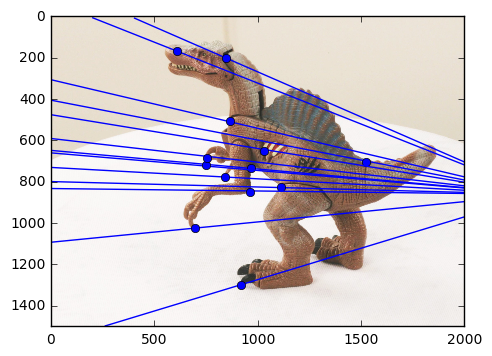
\includegraphics{fig/dinoEpi1.png}
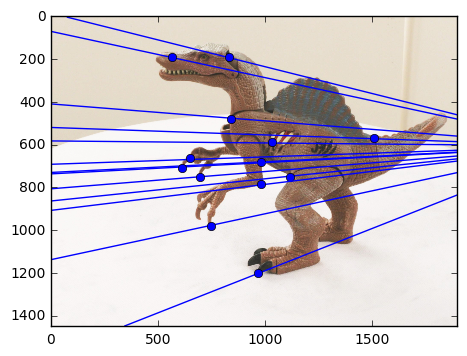
\includegraphics{fig/dinoEpi2.png}

Also, write the script to calculate the epipoles for a given Fundamental
matrix and corner point correspondences in the two images.

    \begin{tcolorbox}[breakable, size=fbox, boxrule=1pt, pad at break*=1mm,colback=cellbackground, colframe=cellborder]
\prompt{In}{incolor}{174}{\boxspacing}
\begin{Verbatim}[commandchars=\\\{\}]
\PY{k}{def} \PY{n+nf}{compute\PYZus{}epipole}\PY{p}{(}\PY{n}{F}\PY{p}{)}\PY{p}{:}
    \PY{l+s+sd}{\PYZsq{}\PYZsq{}\PYZsq{}}
\PY{l+s+sd}{    This function computes the epipoles for a given fundamental matrix }
\PY{l+s+sd}{    and corner point correspondences}
\PY{l+s+sd}{    input:}
\PY{l+s+sd}{    F\PYZhy{}\PYZhy{}\PYZgt{} Fundamental matrix}
\PY{l+s+sd}{    output:}
\PY{l+s+sd}{    e1\PYZhy{}\PYZhy{}\PYZgt{} corresponding epipole in image 1}
\PY{l+s+sd}{    e2\PYZhy{}\PYZhy{}\PYZgt{} epipole in image2}
\PY{l+s+sd}{    \PYZsq{}\PYZsq{}\PYZsq{}}
    \PY{c+c1}{\PYZsh{}your code here}
   
    \PY{n}{e1} \PY{o}{=} \PY{n}{scipy}\PY{o}{.}\PY{n}{linalg}\PY{o}{.}\PY{n}{null\PYZus{}space}\PY{p}{(}\PY{n}{F}\PY{p}{)}
    \PY{n}{e2} \PY{o}{=} \PY{n}{scipy}\PY{o}{.}\PY{n}{linalg}\PY{o}{.}\PY{n}{null\PYZus{}space}\PY{p}{(}\PY{n}{F}\PY{o}{.}\PY{n}{T}\PY{p}{)}
    \PY{k}{return} \PY{n}{e1}\PY{p}{,}\PY{n}{e2}

\PY{k}{def} \PY{n+nf}{plot\PYZus{}epipolar\PYZus{}lines}\PY{p}{(}\PY{n}{img1}\PY{p}{,}\PY{n}{img2}\PY{p}{,} \PY{n}{cor1}\PY{p}{,} \PY{n}{cor2}\PY{p}{)}\PY{p}{:}
    \PY{l+s+sd}{\PYZdq{}\PYZdq{}\PYZdq{}Plot epipolar lines on image given image, corners}

\PY{l+s+sd}{    Args:}
\PY{l+s+sd}{        img1: Image 1.}
\PY{l+s+sd}{        img2: Image 2.}
\PY{l+s+sd}{        cor1: Corners in homogeneous image coordinate in image 1 (3xn)}
\PY{l+s+sd}{        cor2: Corners in homogeneous image coordinate in image 2 (3xn)}

\PY{l+s+sd}{    \PYZdq{}\PYZdq{}\PYZdq{}}
    
    \PY{l+s+sd}{\PYZdq{}\PYZdq{}\PYZdq{}}
\PY{l+s+sd}{    Your code here:}
\PY{l+s+sd}{    \PYZdq{}\PYZdq{}\PYZdq{}}
    
    \PY{n}{F} \PY{o}{=} \PY{n}{calculate\PYZus{}fundamental\PYZus{}matrix}\PY{p}{(}\PY{n}{cor1}\PY{o}{.}\PY{n}{T}\PY{p}{,}\PY{n}{cor2}\PY{o}{.}\PY{n}{T}\PY{p}{)}
    \PY{c+c1}{\PYZsh{}F = fundamental\PYZus{}matrix(cor1,cor2)}
    \PY{n}{fig} \PY{o}{=} \PY{n}{plt}\PY{o}{.}\PY{n}{figure}\PY{p}{(}\PY{p}{)}
    \PY{n}{plt}\PY{o}{.}\PY{n}{ylim}\PY{p}{(}\PY{n}{img1}\PY{o}{.}\PY{n}{shape}\PY{p}{[}\PY{l+m+mi}{0}\PY{p}{]}\PY{p}{,}\PY{l+m+mi}{0}\PY{p}{)}
    \PY{n}{plt}\PY{o}{.}\PY{n}{xlim}\PY{p}{(}\PY{l+m+mi}{0}\PY{p}{,}\PY{n}{img1}\PY{o}{.}\PY{n}{shape}\PY{p}{[}\PY{l+m+mi}{1}\PY{p}{]}\PY{p}{)}
    \PY{n}{x} \PY{o}{=} \PY{n}{np}\PY{o}{.}\PY{n}{linspace}\PY{p}{(}\PY{l+m+mi}{0}\PY{p}{,}\PY{n}{img1}\PY{o}{.}\PY{n}{shape}\PY{p}{[}\PY{l+m+mi}{1}\PY{p}{]}\PY{p}{)}
    \PY{n}{plt}\PY{o}{.}\PY{n}{imshow}\PY{p}{(}\PY{n}{img1}\PY{p}{)}
    \PY{n}{plt}\PY{o}{.}\PY{n}{scatter}\PY{p}{(}\PY{n}{cor1}\PY{p}{[}\PY{l+m+mi}{0}\PY{p}{,}\PY{p}{:}\PY{p}{]}\PY{p}{,}\PY{n}{cor1}\PY{p}{[}\PY{l+m+mi}{1}\PY{p}{,}\PY{p}{:}\PY{p}{]}\PY{p}{)}
    \PY{n}{vals1} \PY{o}{=} \PY{n}{np}\PY{o}{.}\PY{n}{zeros}\PY{p}{(}\PY{n}{cor2}\PY{o}{.}\PY{n}{shape}\PY{p}{)}
    \PY{k}{for} \PY{n}{i} \PY{o+ow}{in} \PY{n+nb}{range}\PY{p}{(}\PY{n}{cor2}\PY{o}{.}\PY{n}{shape}\PY{p}{[}\PY{l+m+mi}{1}\PY{p}{]}\PY{p}{)}\PY{p}{:}
        \PY{n}{vals1}\PY{p}{[}\PY{p}{:}\PY{p}{,}\PY{n}{i}\PY{p}{]} \PY{o}{=} \PY{n}{np}\PY{o}{.}\PY{n}{matmul}\PY{p}{(}\PY{n}{F}\PY{p}{,}\PY{n}{cor1}\PY{p}{[}\PY{p}{:}\PY{p}{,}\PY{n}{i}\PY{p}{]}\PY{p}{)}
    \PY{k}{for} \PY{n}{i} \PY{o+ow}{in} \PY{n+nb}{range}\PY{p}{(}\PY{n}{vals1}\PY{o}{.}\PY{n}{shape}\PY{p}{[}\PY{l+m+mi}{1}\PY{p}{]}\PY{p}{)}\PY{p}{:}
        \PY{n}{y} \PY{o}{=} \PY{o}{\PYZhy{}}\PY{l+m+mi}{1}\PY{o}{*}\PY{n}{x}\PY{o}{*}\PY{n}{vals1}\PY{p}{[}\PY{l+m+mi}{0}\PY{p}{,}\PY{n}{i}\PY{p}{]}\PY{o}{/}\PY{n}{vals1}\PY{p}{[}\PY{l+m+mi}{1}\PY{p}{,}\PY{n}{i}\PY{p}{]} \PY{o}{\PYZhy{}} \PY{n}{vals1}\PY{p}{[}\PY{l+m+mi}{2}\PY{p}{,}\PY{n}{i}\PY{p}{]}\PY{o}{/}\PY{n}{vals1}\PY{p}{[}\PY{l+m+mi}{1}\PY{p}{,}\PY{n}{i}\PY{p}{]}
        \PY{n}{plt}\PY{o}{.}\PY{n}{plot}\PY{p}{(}\PY{n}{x}\PY{p}{,}\PY{n}{y}\PY{p}{,}\PY{l+s+s1}{\PYZsq{}}\PY{l+s+s1}{b}\PY{l+s+s1}{\PYZsq{}}\PY{p}{)}
    
    
    \PY{n}{plt}\PY{o}{.}\PY{n}{show}\PY{p}{(}\PY{p}{)}
    
    \PY{n}{fig} \PY{o}{=} \PY{n}{plt}\PY{o}{.}\PY{n}{figure}\PY{p}{(}\PY{p}{)}
    \PY{n}{plt}\PY{o}{.}\PY{n}{ylim}\PY{p}{(}\PY{n}{img2}\PY{o}{.}\PY{n}{shape}\PY{p}{[}\PY{l+m+mi}{0}\PY{p}{]}\PY{p}{,}\PY{l+m+mi}{0}\PY{p}{)}
    \PY{n}{plt}\PY{o}{.}\PY{n}{xlim}\PY{p}{(}\PY{l+m+mi}{0}\PY{p}{,}\PY{n}{img2}\PY{o}{.}\PY{n}{shape}\PY{p}{[}\PY{l+m+mi}{1}\PY{p}{]}\PY{p}{)}
    \PY{n}{x} \PY{o}{=} \PY{n}{np}\PY{o}{.}\PY{n}{linspace}\PY{p}{(}\PY{l+m+mi}{0}\PY{p}{,}\PY{n}{img2}\PY{o}{.}\PY{n}{shape}\PY{p}{[}\PY{l+m+mi}{1}\PY{p}{]}\PY{p}{)}
    \PY{n}{plt}\PY{o}{.}\PY{n}{imshow}\PY{p}{(}\PY{n}{img2}\PY{p}{)}
    \PY{n}{plt}\PY{o}{.}\PY{n}{scatter}\PY{p}{(}\PY{n}{cor2}\PY{p}{[}\PY{l+m+mi}{0}\PY{p}{,}\PY{p}{:}\PY{p}{]}\PY{p}{,}\PY{n}{cor2}\PY{p}{[}\PY{l+m+mi}{1}\PY{p}{,}\PY{p}{:}\PY{p}{]}\PY{p}{)}
    \PY{n}{vals2} \PY{o}{=} \PY{n}{np}\PY{o}{.}\PY{n}{zeros}\PY{p}{(}\PY{n}{cor1}\PY{o}{.}\PY{n}{shape}\PY{p}{)}
    \PY{k}{for} \PY{n}{i} \PY{o+ow}{in} \PY{n+nb}{range}\PY{p}{(}\PY{n}{cor1}\PY{o}{.}\PY{n}{shape}\PY{p}{[}\PY{l+m+mi}{1}\PY{p}{]}\PY{p}{)}\PY{p}{:}
        \PY{n}{vals2}\PY{p}{[}\PY{p}{:}\PY{p}{,}\PY{n}{i}\PY{p}{]} \PY{o}{=} \PY{n}{np}\PY{o}{.}\PY{n}{matmul}\PY{p}{(}\PY{n}{F}\PY{p}{,}\PY{n}{cor2}\PY{p}{[}\PY{p}{:}\PY{p}{,}\PY{n}{i}\PY{p}{]}\PY{p}{)}
    \PY{k}{for} \PY{n}{i} \PY{o+ow}{in} \PY{n+nb}{range}\PY{p}{(}\PY{n}{vals2}\PY{o}{.}\PY{n}{shape}\PY{p}{[}\PY{l+m+mi}{1}\PY{p}{]}\PY{p}{)}\PY{p}{:}
        \PY{n}{y} \PY{o}{=} \PY{p}{(}\PY{o}{\PYZhy{}}\PY{l+m+mi}{1}\PY{o}{*}\PY{n}{x}\PY{o}{*}\PY{n}{vals2}\PY{p}{[}\PY{l+m+mi}{0}\PY{p}{,}\PY{n}{i}\PY{p}{]} \PY{o}{\PYZhy{}} \PY{n}{vals2}\PY{p}{[}\PY{l+m+mi}{2}\PY{p}{,}\PY{n}{i}\PY{p}{]}\PY{p}{)}\PY{o}{/}\PY{n}{vals2}\PY{p}{[}\PY{l+m+mi}{1}\PY{p}{,}\PY{n}{i}\PY{p}{]}
        \PY{n}{plt}\PY{o}{.}\PY{n}{plot}\PY{p}{(}\PY{n}{x}\PY{p}{,}\PY{n}{y}\PY{p}{,}\PY{l+s+s1}{\PYZsq{}}\PY{l+s+s1}{b}\PY{l+s+s1}{\PYZsq{}}\PY{p}{)}

    \PY{n}{plt}\PY{o}{.}\PY{n}{show}\PY{p}{(}\PY{p}{)}
    
    
\end{Verbatim}
\end{tcolorbox}

    \begin{tcolorbox}[breakable, size=fbox, boxrule=1pt, pad at break*=1mm,colback=cellbackground, colframe=cellborder]
\prompt{In}{incolor}{175}{\boxspacing}
\begin{Verbatim}[commandchars=\\\{\}]
\PY{c+c1}{\PYZsh{} replace images and corners with those of matrix and warrior}
\PY{n}{imgids} \PY{o}{=} \PY{p}{[}\PY{l+s+s2}{\PYZdq{}}\PY{l+s+s2}{matrix}\PY{l+s+s2}{\PYZdq{}}\PY{p}{,} \PY{l+s+s2}{\PYZdq{}}\PY{l+s+s2}{warrior}\PY{l+s+s2}{\PYZdq{}}\PY{p}{]}
\PY{k}{for} \PY{n}{imgid} \PY{o+ow}{in} \PY{n}{imgids}\PY{p}{:}
    \PY{n}{I1} \PY{o}{=} \PY{n}{imageio}\PY{o}{.}\PY{n}{imread}\PY{p}{(}\PY{l+s+s2}{\PYZdq{}}\PY{l+s+s2}{./p4/}\PY{l+s+s2}{\PYZdq{}}\PY{o}{+}\PY{n}{imgid}\PY{o}{+}\PY{l+s+s2}{\PYZdq{}}\PY{l+s+s2}{/}\PY{l+s+s2}{\PYZdq{}}\PY{o}{+}\PY{n}{imgid}\PY{o}{+}\PY{l+s+s2}{\PYZdq{}}\PY{l+s+s2}{0.png}\PY{l+s+s2}{\PYZdq{}}\PY{p}{)}
    \PY{n}{I2} \PY{o}{=} \PY{n}{imageio}\PY{o}{.}\PY{n}{imread}\PY{p}{(}\PY{l+s+s2}{\PYZdq{}}\PY{l+s+s2}{./p4/}\PY{l+s+s2}{\PYZdq{}}\PY{o}{+}\PY{n}{imgid}\PY{o}{+}\PY{l+s+s2}{\PYZdq{}}\PY{l+s+s2}{/}\PY{l+s+s2}{\PYZdq{}}\PY{o}{+}\PY{n}{imgid}\PY{o}{+}\PY{l+s+s2}{\PYZdq{}}\PY{l+s+s2}{1.png}\PY{l+s+s2}{\PYZdq{}}\PY{p}{)}

    \PY{n}{cor1} \PY{o}{=} \PY{n}{np}\PY{o}{.}\PY{n}{load}\PY{p}{(}\PY{l+s+s2}{\PYZdq{}}\PY{l+s+s2}{./p4/}\PY{l+s+s2}{\PYZdq{}}\PY{o}{+}\PY{n}{imgid}\PY{o}{+}\PY{l+s+s2}{\PYZdq{}}\PY{l+s+s2}{/cor1.npy}\PY{l+s+s2}{\PYZdq{}}\PY{p}{)}
    \PY{n}{cor2} \PY{o}{=} \PY{n}{np}\PY{o}{.}\PY{n}{load}\PY{p}{(}\PY{l+s+s2}{\PYZdq{}}\PY{l+s+s2}{./p4/}\PY{l+s+s2}{\PYZdq{}}\PY{o}{+}\PY{n}{imgid}\PY{o}{+}\PY{l+s+s2}{\PYZdq{}}\PY{l+s+s2}{/cor2.npy}\PY{l+s+s2}{\PYZdq{}}\PY{p}{)}
    \PY{n}{plot\PYZus{}epipolar\PYZus{}lines}\PY{p}{(}\PY{n}{I1}\PY{p}{,}\PY{n}{I2}\PY{p}{,}\PY{n}{cor1}\PY{p}{,}\PY{n}{cor2}\PY{p}{)}
\end{Verbatim}
\end{tcolorbox}

    \begin{center}
    \adjustimage{max size={0.9\linewidth}{0.9\paperheight}}{output_25_0.png}
    \end{center}
    { \hspace*{\fill} \\}
    
    \begin{center}
    \adjustimage{max size={0.9\linewidth}{0.9\paperheight}}{output_25_1.png}
    \end{center}
    { \hspace*{\fill} \\}
    
    \begin{center}
    \adjustimage{max size={0.9\linewidth}{0.9\paperheight}}{output_25_2.png}
    \end{center}
    { \hspace*{\fill} \\}
    
    \begin{center}
    \adjustimage{max size={0.9\linewidth}{0.9\paperheight}}{output_25_3.png}
    \end{center}
    { \hspace*{\fill} \\}
    
    \hypertarget{image-rectification-5-pts}{%
\subsubsection{Image Rectification {[}5
pts{]}}\label{image-rectification-5-pts}}

An interesting case for epipolar geometry occurs when two images are
parallel to each other. In this case, there is no rotation component
involved between the two images and the essential matrix is
\(\texttt{E}=[\boldsymbol{T_{x}}]\boldsymbol{R}=[\boldsymbol{T_{x}}]\).
Also if you observe the epipolar lines \(\boldsymbol{l}\) and
\(\boldsymbol{l^{'}}\) for parallel images, they are horizontal and
consequently, the corresponding epipolar lines share the same vertical
coordinate. Therefore the process of making images parallel becomes
useful while discerning the relationships between corresponding points
in images. Rectifying a pair of images can also be done for uncalibrated
camera images (i.e.~we do not require the camera matrix of intrinsic
parameters). Using the fundamental matrix we can find the pair of
epipolar lines \(\boldsymbol{l_i}\) and \(\boldsymbol{l^{'}_i}\) for
each of the correspondences. The intersection of these lines will give
us the respective epipoles \(\boldsymbol{e}\) and
\(\boldsymbol{e^{'}}\). Now to make the epipolar lines to be parallel we
need to map the epipoles to infinity. Hence , we need to find a
homography that maps the epipoles to infinity. The method to find the
homography has been implemented for you. You can read more about the
method used to estimate the homography in the paper ``Theory and
Practice of Projective Rectification'' by Richard Hartley.
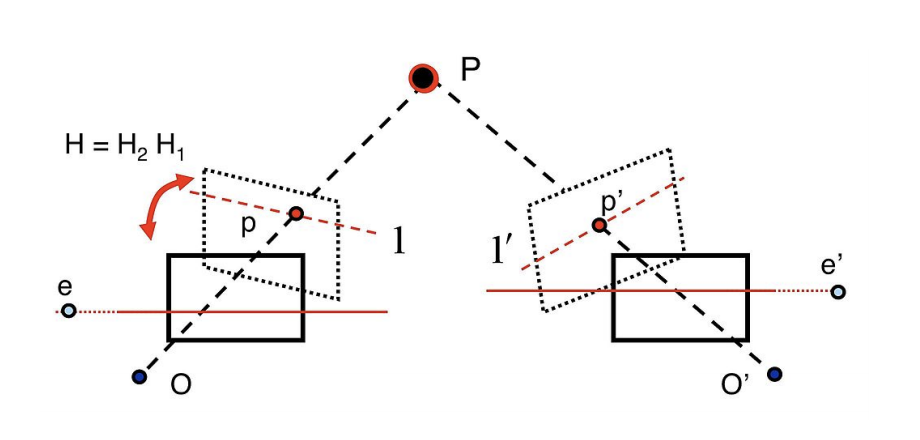
\includegraphics{image_rectification.png} Using the compute\_epipoles
function from the previous part and the given
compute\_matching\_homographies function, find the rectified images and
plot the parallel epipolar lines using the plot\_epipolar\_lines
function from above. You need to do this for both the matrix and the
warrior images. A sample output will look as below:
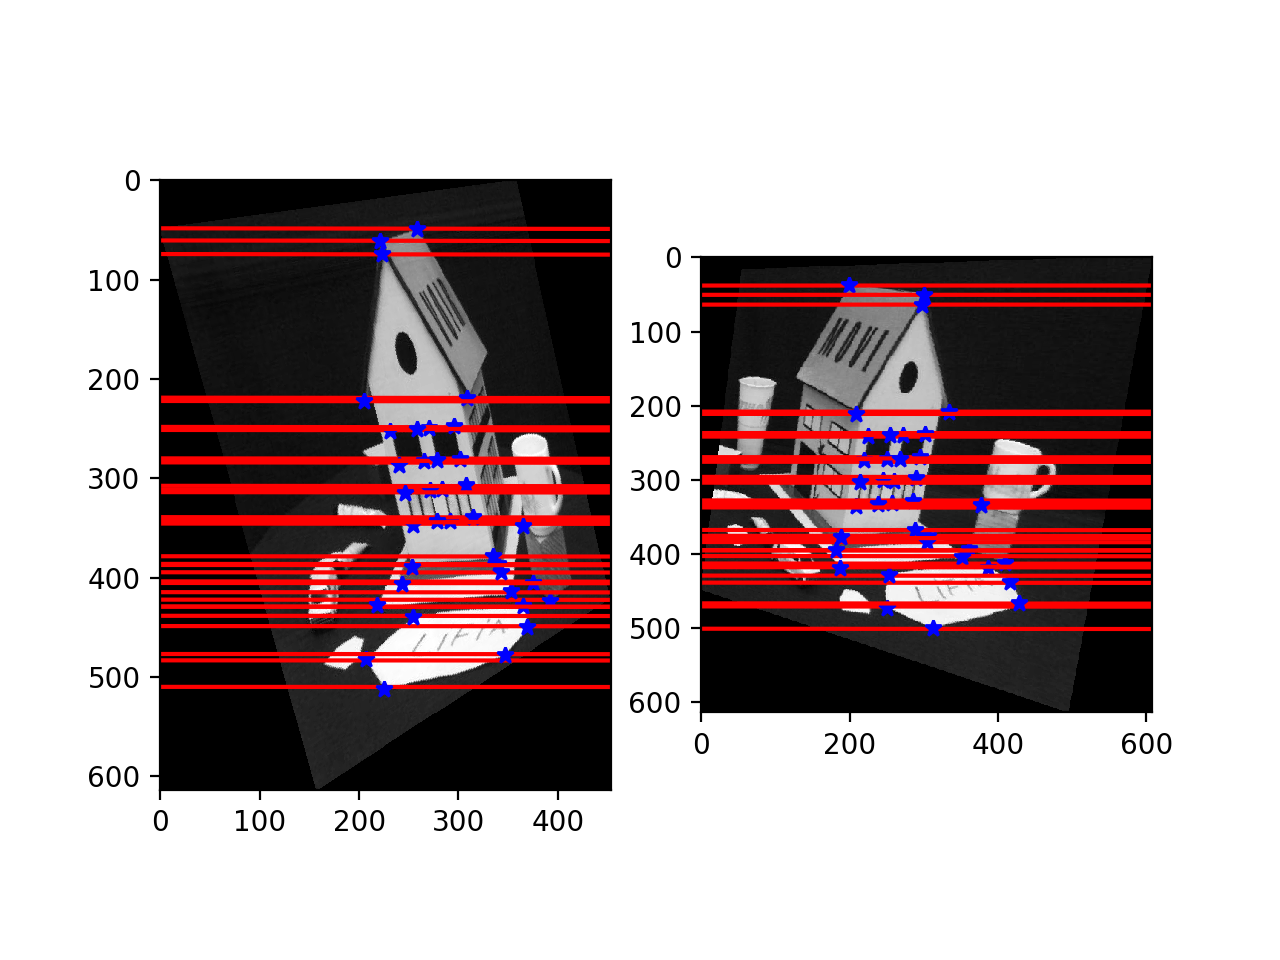
\includegraphics{Sample_rectification.png}

    \begin{tcolorbox}[breakable, size=fbox, boxrule=1pt, pad at break*=1mm,colback=cellbackground, colframe=cellborder]
\prompt{In}{incolor}{176}{\boxspacing}
\begin{Verbatim}[commandchars=\\\{\}]
\PY{k+kn}{import} \PY{n+nn}{math}
\PY{k}{def} \PY{n+nf}{compute\PYZus{}matching\PYZus{}homographies}\PY{p}{(}\PY{n}{e2}\PY{p}{,} \PY{n}{F}\PY{p}{,} \PY{n}{im2}\PY{p}{,} \PY{n}{points1}\PY{p}{,} \PY{n}{points2}\PY{p}{)}\PY{p}{:}
    
    \PY{l+s+sd}{\PYZsq{}\PYZsq{}\PYZsq{}This function computes the homographies to get the rectified images}
\PY{l+s+sd}{    input:}
\PY{l+s+sd}{    e2\PYZhy{}\PYZhy{}\PYZgt{} epipole in image 2}
\PY{l+s+sd}{    F\PYZhy{}\PYZhy{}\PYZgt{} the Fundamental matrix (Think about what you should be passing F or F.T!)}
\PY{l+s+sd}{    im2\PYZhy{}\PYZhy{}\PYZgt{} image2}
\PY{l+s+sd}{    points1 \PYZhy{}\PYZhy{}\PYZgt{} corner points in image1}
\PY{l+s+sd}{    points2\PYZhy{}\PYZhy{}\PYZgt{} corresponding corner points in image2}
\PY{l+s+sd}{    output:}
\PY{l+s+sd}{    H1\PYZhy{}\PYZhy{}\PYZgt{} Homography for image 1}
\PY{l+s+sd}{    H2\PYZhy{}\PYZhy{}\PYZgt{} Homography for image 2}
\PY{l+s+sd}{    \PYZsq{}\PYZsq{}\PYZsq{}}
    \PY{c+c1}{\PYZsh{} calculate H2}
    \PY{n}{width} \PY{o}{=} \PY{n}{im2}\PY{o}{.}\PY{n}{shape}\PY{p}{[}\PY{l+m+mi}{1}\PY{p}{]}
    \PY{n}{height} \PY{o}{=} \PY{n}{im2}\PY{o}{.}\PY{n}{shape}\PY{p}{[}\PY{l+m+mi}{0}\PY{p}{]}

    \PY{n}{T} \PY{o}{=} \PY{n}{np}\PY{o}{.}\PY{n}{identity}\PY{p}{(}\PY{l+m+mi}{3}\PY{p}{)}
    \PY{n}{T}\PY{p}{[}\PY{l+m+mi}{0}\PY{p}{]}\PY{p}{[}\PY{l+m+mi}{2}\PY{p}{]} \PY{o}{=} \PY{o}{\PYZhy{}}\PY{l+m+mf}{1.0} \PY{o}{*} \PY{n}{width} \PY{o}{/} \PY{l+m+mi}{2}
    \PY{n}{T}\PY{p}{[}\PY{l+m+mi}{1}\PY{p}{]}\PY{p}{[}\PY{l+m+mi}{2}\PY{p}{]} \PY{o}{=} \PY{o}{\PYZhy{}}\PY{l+m+mf}{1.0} \PY{o}{*} \PY{n}{height} \PY{o}{/} \PY{l+m+mi}{2}

    \PY{n}{e} \PY{o}{=} \PY{n}{T}\PY{o}{.}\PY{n}{dot}\PY{p}{(}\PY{n}{e2}\PY{p}{)}
    \PY{n}{e1\PYZus{}prime} \PY{o}{=} \PY{n}{e}\PY{p}{[}\PY{l+m+mi}{0}\PY{p}{]}
    \PY{n}{e2\PYZus{}prime} \PY{o}{=} \PY{n}{e}\PY{p}{[}\PY{l+m+mi}{1}\PY{p}{]}
    \PY{k}{if} \PY{n}{e1\PYZus{}prime} \PY{o}{\PYZgt{}}\PY{o}{=} \PY{l+m+mi}{0}\PY{p}{:}
        \PY{n}{alpha} \PY{o}{=} \PY{l+m+mf}{1.0}
    \PY{k}{else}\PY{p}{:}
        \PY{n}{alpha} \PY{o}{=} \PY{o}{\PYZhy{}}\PY{l+m+mf}{1.0}

    \PY{n}{R} \PY{o}{=} \PY{n}{np}\PY{o}{.}\PY{n}{identity}\PY{p}{(}\PY{l+m+mi}{3}\PY{p}{)}
    \PY{n}{R}\PY{p}{[}\PY{l+m+mi}{0}\PY{p}{]}\PY{p}{[}\PY{l+m+mi}{0}\PY{p}{]} \PY{o}{=} \PY{n}{alpha} \PY{o}{*} \PY{n}{e1\PYZus{}prime} \PY{o}{/} \PY{n}{np}\PY{o}{.}\PY{n}{sqrt}\PY{p}{(}\PY{n}{e1\PYZus{}prime}\PY{o}{*}\PY{o}{*}\PY{l+m+mi}{2} \PY{o}{+} \PY{n}{e2\PYZus{}prime}\PY{o}{*}\PY{o}{*}\PY{l+m+mi}{2}\PY{p}{)}
    \PY{n}{R}\PY{p}{[}\PY{l+m+mi}{0}\PY{p}{]}\PY{p}{[}\PY{l+m+mi}{1}\PY{p}{]} \PY{o}{=} \PY{n}{alpha} \PY{o}{*} \PY{n}{e2\PYZus{}prime} \PY{o}{/} \PY{n}{np}\PY{o}{.}\PY{n}{sqrt}\PY{p}{(}\PY{n}{e1\PYZus{}prime}\PY{o}{*}\PY{o}{*}\PY{l+m+mi}{2} \PY{o}{+} \PY{n}{e2\PYZus{}prime}\PY{o}{*}\PY{o}{*}\PY{l+m+mi}{2}\PY{p}{)}
    \PY{n}{R}\PY{p}{[}\PY{l+m+mi}{1}\PY{p}{]}\PY{p}{[}\PY{l+m+mi}{0}\PY{p}{]} \PY{o}{=} \PY{o}{\PYZhy{}} \PY{n}{alpha} \PY{o}{*} \PY{n}{e2\PYZus{}prime} \PY{o}{/} \PY{n}{np}\PY{o}{.}\PY{n}{sqrt}\PY{p}{(}\PY{n}{e1\PYZus{}prime}\PY{o}{*}\PY{o}{*}\PY{l+m+mi}{2} \PY{o}{+} \PY{n}{e2\PYZus{}prime}\PY{o}{*}\PY{o}{*}\PY{l+m+mi}{2}\PY{p}{)}
    \PY{n}{R}\PY{p}{[}\PY{l+m+mi}{1}\PY{p}{]}\PY{p}{[}\PY{l+m+mi}{1}\PY{p}{]} \PY{o}{=} \PY{n}{alpha} \PY{o}{*} \PY{n}{e1\PYZus{}prime} \PY{o}{/} \PY{n}{np}\PY{o}{.}\PY{n}{sqrt}\PY{p}{(}\PY{n}{e1\PYZus{}prime}\PY{o}{*}\PY{o}{*}\PY{l+m+mi}{2} \PY{o}{+} \PY{n}{e2\PYZus{}prime}\PY{o}{*}\PY{o}{*}\PY{l+m+mi}{2}\PY{p}{)}

    \PY{n}{f} \PY{o}{=} \PY{n}{R}\PY{o}{.}\PY{n}{dot}\PY{p}{(}\PY{n}{e}\PY{p}{)}\PY{p}{[}\PY{l+m+mi}{0}\PY{p}{]}\PY{o}{/}\PY{n}{R}\PY{o}{.}\PY{n}{dot}\PY{p}{(}\PY{n}{e}\PY{p}{)}\PY{p}{[}\PY{l+m+mi}{2}\PY{p}{]}
    \PY{n}{G} \PY{o}{=} \PY{n}{np}\PY{o}{.}\PY{n}{identity}\PY{p}{(}\PY{l+m+mi}{3}\PY{p}{)}
    \PY{n}{G}\PY{p}{[}\PY{l+m+mi}{2}\PY{p}{]}\PY{p}{[}\PY{l+m+mi}{0}\PY{p}{]} \PY{o}{=} \PY{o}{\PYZhy{}} \PY{l+m+mf}{1.0} \PY{o}{/} \PY{n}{f}

    \PY{n}{H2} \PY{o}{=} \PY{n}{np}\PY{o}{.}\PY{n}{linalg}\PY{o}{.}\PY{n}{inv}\PY{p}{(}\PY{n}{T}\PY{p}{)}\PY{o}{.}\PY{n}{dot}\PY{p}{(}\PY{n}{G}\PY{o}{.}\PY{n}{dot}\PY{p}{(}\PY{n}{R}\PY{o}{.}\PY{n}{dot}\PY{p}{(}\PY{n}{T}\PY{p}{)}\PY{p}{)}\PY{p}{)}

    \PY{c+c1}{\PYZsh{} calculate H1}
    \PY{n}{e\PYZus{}prime} \PY{o}{=} \PY{n}{np}\PY{o}{.}\PY{n}{zeros}\PY{p}{(}\PY{p}{(}\PY{l+m+mi}{3}\PY{p}{,} \PY{l+m+mi}{3}\PY{p}{)}\PY{p}{)}
    \PY{n}{e\PYZus{}prime}\PY{p}{[}\PY{l+m+mi}{0}\PY{p}{]}\PY{p}{[}\PY{l+m+mi}{1}\PY{p}{]} \PY{o}{=} \PY{o}{\PYZhy{}}\PY{n}{e2}\PY{p}{[}\PY{l+m+mi}{2}\PY{p}{]}
    \PY{n}{e\PYZus{}prime}\PY{p}{[}\PY{l+m+mi}{0}\PY{p}{]}\PY{p}{[}\PY{l+m+mi}{2}\PY{p}{]} \PY{o}{=} \PY{n}{e2}\PY{p}{[}\PY{l+m+mi}{1}\PY{p}{]}
    \PY{n}{e\PYZus{}prime}\PY{p}{[}\PY{l+m+mi}{1}\PY{p}{]}\PY{p}{[}\PY{l+m+mi}{0}\PY{p}{]} \PY{o}{=} \PY{n}{e2}\PY{p}{[}\PY{l+m+mi}{2}\PY{p}{]}
    \PY{n}{e\PYZus{}prime}\PY{p}{[}\PY{l+m+mi}{1}\PY{p}{]}\PY{p}{[}\PY{l+m+mi}{2}\PY{p}{]} \PY{o}{=} \PY{o}{\PYZhy{}}\PY{n}{e2}\PY{p}{[}\PY{l+m+mi}{0}\PY{p}{]}
    \PY{n}{e\PYZus{}prime}\PY{p}{[}\PY{l+m+mi}{2}\PY{p}{]}\PY{p}{[}\PY{l+m+mi}{0}\PY{p}{]} \PY{o}{=} \PY{o}{\PYZhy{}}\PY{n}{e2}\PY{p}{[}\PY{l+m+mi}{1}\PY{p}{]}
    \PY{n}{e\PYZus{}prime}\PY{p}{[}\PY{l+m+mi}{2}\PY{p}{]}\PY{p}{[}\PY{l+m+mi}{1}\PY{p}{]} \PY{o}{=} \PY{n}{e2}\PY{p}{[}\PY{l+m+mi}{0}\PY{p}{]}

    \PY{n}{v} \PY{o}{=} \PY{n}{np}\PY{o}{.}\PY{n}{array}\PY{p}{(}\PY{p}{[}\PY{l+m+mi}{1}\PY{p}{,} \PY{l+m+mi}{1}\PY{p}{,} \PY{l+m+mi}{1}\PY{p}{]}\PY{p}{)}
    \PY{n}{M} \PY{o}{=} \PY{n}{e\PYZus{}prime}\PY{o}{.}\PY{n}{dot}\PY{p}{(}\PY{n}{F}\PY{p}{)} \PY{o}{+} \PY{n}{np}\PY{o}{.}\PY{n}{outer}\PY{p}{(}\PY{n}{e2}\PY{p}{,} \PY{n}{v}\PY{p}{)}

    \PY{n}{points1\PYZus{}hat} \PY{o}{=} \PY{n}{H2}\PY{o}{.}\PY{n}{dot}\PY{p}{(}\PY{n}{M}\PY{o}{.}\PY{n}{dot}\PY{p}{(}\PY{n}{points1}\PY{o}{.}\PY{n}{T}\PY{p}{)}\PY{p}{)}\PY{o}{.}\PY{n}{T}
    \PY{n}{points2\PYZus{}hat} \PY{o}{=} \PY{n}{H2}\PY{o}{.}\PY{n}{dot}\PY{p}{(}\PY{n}{points2}\PY{o}{.}\PY{n}{T}\PY{p}{)}\PY{o}{.}\PY{n}{T}

    \PY{n}{W} \PY{o}{=} \PY{n}{points1\PYZus{}hat} \PY{o}{/} \PY{n}{points1\PYZus{}hat}\PY{p}{[}\PY{p}{:}\PY{p}{,} \PY{l+m+mi}{2}\PY{p}{]}\PY{o}{.}\PY{n}{reshape}\PY{p}{(}\PY{o}{\PYZhy{}}\PY{l+m+mi}{1}\PY{p}{,} \PY{l+m+mi}{1}\PY{p}{)}
    \PY{n}{b} \PY{o}{=} \PY{p}{(}\PY{n}{points2\PYZus{}hat} \PY{o}{/} \PY{n}{points2\PYZus{}hat}\PY{p}{[}\PY{p}{:}\PY{p}{,} \PY{l+m+mi}{2}\PY{p}{]}\PY{o}{.}\PY{n}{reshape}\PY{p}{(}\PY{o}{\PYZhy{}}\PY{l+m+mi}{1}\PY{p}{,} \PY{l+m+mi}{1}\PY{p}{)}\PY{p}{)}\PY{p}{[}\PY{p}{:}\PY{p}{,} \PY{l+m+mi}{0}\PY{p}{]}

    \PY{c+c1}{\PYZsh{} least square problem}
    \PY{n}{a1}\PY{p}{,} \PY{n}{a2}\PY{p}{,} \PY{n}{a3} \PY{o}{=} \PY{n}{np}\PY{o}{.}\PY{n}{linalg}\PY{o}{.}\PY{n}{lstsq}\PY{p}{(}\PY{n}{W}\PY{p}{,} \PY{n}{b}\PY{p}{,} \PY{n}{rcond}\PY{o}{=}\PY{k+kc}{None}\PY{p}{)}\PY{p}{[}\PY{l+m+mi}{0}\PY{p}{]}
    \PY{n}{HA} \PY{o}{=} \PY{n}{np}\PY{o}{.}\PY{n}{identity}\PY{p}{(}\PY{l+m+mi}{3}\PY{p}{)}
    \PY{n}{HA}\PY{p}{[}\PY{l+m+mi}{0}\PY{p}{]} \PY{o}{=} \PY{n}{np}\PY{o}{.}\PY{n}{array}\PY{p}{(}\PY{p}{[}\PY{n}{a1}\PY{p}{,} \PY{n}{a2}\PY{p}{,} \PY{n}{a3}\PY{p}{]}\PY{p}{)}

    \PY{n}{H1} \PY{o}{=} \PY{n}{HA}\PY{o}{.}\PY{n}{dot}\PY{p}{(}\PY{n}{H2}\PY{p}{)}\PY{o}{.}\PY{n}{dot}\PY{p}{(}\PY{n}{M}\PY{p}{)}
    \PY{k}{return} \PY{n}{H1}\PY{p}{,} \PY{n}{H2}

\PY{k}{def} \PY{n+nf}{computeH}\PY{p}{(}\PY{n}{source\PYZus{}points}\PY{p}{,} \PY{n}{target\PYZus{}points}\PY{p}{)}\PY{p}{:}
    \PY{c+c1}{\PYZsh{} returns the 3x3 homography matrix such that:}
    \PY{c+c1}{\PYZsh{} np.matmul(H, source\PYZus{}points) = target\PYZus{}points}
    \PY{c+c1}{\PYZsh{} where source\PYZus{}points and target\PYZus{}points are expected to be in homogeneous}
    \PY{c+c1}{\PYZsh{} make sure points are 3D homogeneous}
    \PY{k}{assert} \PY{n}{source\PYZus{}points}\PY{o}{.}\PY{n}{shape}\PY{p}{[}\PY{l+m+mi}{0}\PY{p}{]}\PY{o}{==}\PY{l+m+mi}{3} \PY{o+ow}{and} \PY{n}{target\PYZus{}points}\PY{o}{.}\PY{n}{shape}\PY{p}{[}\PY{l+m+mi}{0}\PY{p}{]}\PY{o}{==}\PY{l+m+mi}{3}
    \PY{c+c1}{\PYZsh{}compute H\PYZca{}\PYZhy{}1}
    \PY{n}{source\PYZus{}x1x2x3} \PY{o}{=} \PY{n}{source\PYZus{}points}\PY{p}{[}\PY{p}{:}\PY{p}{,}\PY{p}{:}\PY{l+m+mi}{3}\PY{p}{]}
    \PY{n}{source\PYZus{}x4} \PY{o}{=} \PY{n}{source\PYZus{}points}\PY{p}{[}\PY{p}{:}\PY{p}{,}\PY{o}{\PYZhy{}}\PY{l+m+mi}{1}\PY{p}{:}\PY{p}{]}
    \PY{n}{source\PYZus{}x1x2x3\PYZus{}inv} \PY{o}{=} \PY{n}{np}\PY{o}{.}\PY{n}{linalg}\PY{o}{.}\PY{n}{inv}\PY{p}{(}\PY{n}{source\PYZus{}x1x2x3}\PY{p}{)}
    \PY{n}{source\PYZus{}lambdas} \PY{o}{=} \PY{n}{np}\PY{o}{.}\PY{n}{matmul}\PY{p}{(}\PY{n}{source\PYZus{}x1x2x3\PYZus{}inv}\PY{p}{,}\PY{n}{source\PYZus{}x4}\PY{p}{)}
    \PY{n}{diag\PYZus{}source\PYZus{}lambdas} \PY{o}{=} \PY{n}{np}\PY{o}{.}\PY{n}{array}\PY{p}{(}\PY{p}{[}\PY{p}{[}\PY{n}{source\PYZus{}lambdas}\PY{p}{[}\PY{l+m+mi}{0}\PY{p}{,}\PY{l+m+mi}{0}\PY{p}{]}\PY{p}{,} \PY{l+m+mi}{0}\PY{p}{,} \PY{l+m+mi}{0}\PY{p}{]}\PY{p}{,} \PY{p}{[}\PY{l+m+mi}{0}\PY{p}{,} \PY{n}{source\PYZus{}lambdas}\PY{p}{[}\PY{l+m+mi}{1}\PY{p}{,}\PY{l+m+mi}{0}\PY{p}{]}\PY{p}{,} \PY{l+m+mi}{0}\PY{p}{]}\PY{p}{,} \PY{p}{[}\PY{l+m+mi}{0}\PY{p}{,} \PY{l+m+mi}{0}\PY{p}{,} \PY{n}{source\PYZus{}lambdas}\PY{p}{[}\PY{l+m+mi}{2}\PY{p}{,}\PY{l+m+mi}{0}\PY{p}{]}\PY{p}{]}\PY{p}{]}\PY{p}{)}
    \PY{n}{H\PYZus{}inv1} \PY{o}{=} \PY{n}{np}\PY{o}{.}\PY{n}{matmul}\PY{p}{(}\PY{n}{source\PYZus{}x1x2x3}\PY{p}{,}\PY{n}{diag\PYZus{}source\PYZus{}lambdas}\PY{p}{)}
    \PY{c+c1}{\PYZsh{}computer H\PYZca{}\PYZhy{}2}
    \PY{n}{target\PYZus{}x1x2x3} \PY{o}{=} \PY{n}{target\PYZus{}points}\PY{p}{[}\PY{p}{:}\PY{p}{,}\PY{p}{:}\PY{l+m+mi}{3}\PY{p}{]}
    \PY{n}{target\PYZus{}x4} \PY{o}{=} \PY{n}{target\PYZus{}points}\PY{p}{[}\PY{p}{:}\PY{p}{,}\PY{o}{\PYZhy{}}\PY{l+m+mi}{1}\PY{p}{:}\PY{p}{]}
    \PY{n}{target\PYZus{}x1x2x3\PYZus{}inv} \PY{o}{=} \PY{n}{np}\PY{o}{.}\PY{n}{linalg}\PY{o}{.}\PY{n}{inv}\PY{p}{(}\PY{n}{target\PYZus{}x1x2x3}\PY{p}{)}
    \PY{n}{target\PYZus{}lambdas} \PY{o}{=} \PY{n}{np}\PY{o}{.}\PY{n}{matmul}\PY{p}{(}\PY{n}{target\PYZus{}x1x2x3\PYZus{}inv}\PY{p}{,}\PY{n}{target\PYZus{}x4}\PY{p}{)}
    \PY{n}{diag\PYZus{}target\PYZus{}lambdas} \PY{o}{=} \PY{n}{np}\PY{o}{.}\PY{n}{array}\PY{p}{(}\PY{p}{[}\PY{p}{[}\PY{n}{target\PYZus{}lambdas}\PY{p}{[}\PY{l+m+mi}{0}\PY{p}{,}\PY{l+m+mi}{0}\PY{p}{]}\PY{p}{,} \PY{l+m+mi}{0}\PY{p}{,} \PY{l+m+mi}{0}\PY{p}{]}\PY{p}{,} \PY{p}{[}\PY{l+m+mi}{0}\PY{p}{,} \PY{n}{target\PYZus{}lambdas}\PY{p}{[}\PY{l+m+mi}{1}\PY{p}{,}\PY{l+m+mi}{0}\PY{p}{]}\PY{p}{,} \PY{l+m+mi}{0}\PY{p}{]}\PY{p}{,} \PY{p}{[}\PY{l+m+mi}{0}\PY{p}{,} \PY{l+m+mi}{0}\PY{p}{,} \PY{n}{target\PYZus{}lambdas}\PY{p}{[}\PY{l+m+mi}{2}\PY{p}{,}\PY{l+m+mi}{0}\PY{p}{]}\PY{p}{]}\PY{p}{]}\PY{p}{)}
    \PY{n}{H\PYZus{}inv2} \PY{o}{=} \PY{n}{np}\PY{o}{.}\PY{n}{matmul}\PY{p}{(}\PY{n}{target\PYZus{}x1x2x3}\PY{p}{,}\PY{n}{diag\PYZus{}target\PYZus{}lambdas}\PY{p}{)}
    
    \PY{n}{H\PYZus{}mtx} \PY{o}{=} \PY{n}{np}\PY{o}{.}\PY{n}{matmul}\PY{p}{(}\PY{n}{H\PYZus{}inv2}\PY{p}{,}\PY{n}{np}\PY{o}{.}\PY{n}{linalg}\PY{o}{.}\PY{n}{inv}\PY{p}{(}\PY{n}{H\PYZus{}inv1}\PY{p}{)}\PY{p}{)}

    \PY{k}{return}  \PY{n}{H\PYZus{}mtx}

\PY{k}{def} \PY{n+nf}{to\PYZus{}homog}\PY{p}{(}\PY{n}{points}\PY{p}{)}\PY{p}{:} \PY{c+c1}{\PYZsh{}here always remember that points is a 3x4 matrix}
    \PY{k}{return} \PY{n}{np}\PY{o}{.}\PY{n}{vstack}\PY{p}{(}\PY{p}{(}\PY{n}{points}\PY{p}{,} \PY{n}{points}\PY{p}{[}\PY{l+m+mi}{0}\PY{p}{]}\PY{o}{.}\PY{n}{size} \PY{o}{*} \PY{p}{[}\PY{l+m+mi}{1}\PY{p}{]}\PY{p}{)}\PY{p}{)}
    
\PY{c+c1}{\PYZsh{} convert points from homogeneous to euclidian}
\PY{k}{def} \PY{n+nf}{from\PYZus{}homog}\PY{p}{(}\PY{n}{points\PYZus{}homog}\PY{p}{)}\PY{p}{:}  
    \PY{k}{return}  \PY{n}{points\PYZus{}homog} \PY{o}{/} \PY{n}{points\PYZus{}homog}\PY{p}{[}\PY{o}{\PYZhy{}}\PY{l+m+mi}{1}\PY{p}{,}\PY{p}{:}\PY{p}{]}

    

\PY{k}{def} \PY{n+nf}{warp}\PY{p}{(}\PY{n}{source\PYZus{}img}\PY{p}{,} \PY{n}{H}\PY{p}{,} \PY{n}{target\PYZus{}size}\PY{p}{)}\PY{p}{:}

    \PY{k}{assert} \PY{n}{target\PYZus{}size}\PY{p}{[}\PY{l+m+mi}{2}\PY{p}{]}\PY{o}{==}\PY{n}{source\PYZus{}img}\PY{o}{.}\PY{n}{shape}\PY{p}{[}\PY{l+m+mi}{2}\PY{p}{]}
    
    \PY{n}{target\PYZus{}img} \PY{o}{=} \PY{n}{np}\PY{o}{.}\PY{n}{zeros}\PY{p}{(}\PY{n}{target\PYZus{}size}\PY{p}{,} \PY{n}{dtype}\PY{o}{=}\PY{n+nb}{int}\PY{p}{)}
    
    \PY{k}{for} \PY{n}{i} \PY{o+ow}{in} \PY{n+nb}{range}\PY{p}{(}\PY{n}{source\PYZus{}img}\PY{o}{.}\PY{n}{shape}\PY{p}{[}\PY{l+m+mi}{0}\PY{p}{]}\PY{p}{)}\PY{p}{:}
        \PY{k}{for} \PY{n}{j} \PY{o+ow}{in} \PY{n+nb}{range}\PY{p}{(}\PY{n}{source\PYZus{}img}\PY{o}{.}\PY{n}{shape}\PY{p}{[}\PY{l+m+mi}{1}\PY{p}{]}\PY{p}{)}\PY{p}{:}
            \PY{n}{x\PYZus{}coords} \PY{o}{=} \PY{p}{[}\PY{n}{i}\PY{p}{]} 
            \PY{n}{y\PYZus{}coords} \PY{o}{=} \PY{p}{[}\PY{n}{j}\PY{p}{]}
            \PY{n}{source\PYZus{}points} \PY{o}{=} \PY{n}{np}\PY{o}{.}\PY{n}{vstack}\PY{p}{(}\PY{p}{(}\PY{n}{x\PYZus{}coords}\PY{p}{,} \PY{n}{y\PYZus{}coords}\PY{p}{)}\PY{p}{)}
            \PY{n}{mp} \PY{o}{=} \PY{n}{from\PYZus{}homog}\PY{p}{(}\PY{n}{np}\PY{o}{.}\PY{n}{matmul}\PY{p}{(}\PY{n}{H}\PY{p}{,}\PY{n}{to\PYZus{}homog}\PY{p}{(}\PY{n}{source\PYZus{}points}\PY{p}{)}\PY{p}{)}\PY{p}{)}
            \PY{n}{tx} \PY{o}{=} \PY{n+nb}{int}\PY{p}{(}\PY{n}{math}\PY{o}{.}\PY{n}{floor}\PY{p}{(}\PY{n}{mp}\PY{p}{[}\PY{l+m+mi}{0}\PY{p}{]}\PY{p}{)}\PY{p}{)}
            \PY{n}{ty} \PY{o}{=} \PY{n+nb}{int}\PY{p}{(}\PY{n}{math}\PY{o}{.}\PY{n}{floor}\PY{p}{(}\PY{n}{mp}\PY{p}{[}\PY{l+m+mi}{1}\PY{p}{]}\PY{p}{)}\PY{p}{)}
            \PY{k}{if} \PY{n}{tx} \PY{o}{\PYZlt{}} \PY{n}{target\PYZus{}size}\PY{p}{[}\PY{l+m+mi}{0}\PY{p}{]} \PY{o+ow}{and} \PY{n}{tx} \PY{o}{\PYZgt{}} \PY{l+m+mi}{0} \PY{o+ow}{and} \PY{n}{ty} \PY{o}{\PYZlt{}} \PY{n}{target\PYZus{}size}\PY{p}{[}\PY{l+m+mi}{1}\PY{p}{]} \PY{o+ow}{and} \PY{n}{ty} \PY{o}{\PYZgt{}} \PY{l+m+mi}{0}\PY{p}{:}
                \PY{n}{target\PYZus{}img}\PY{p}{[}\PY{n}{tx}\PY{p}{,}\PY{n}{ty}\PY{p}{]} \PY{o}{=} \PY{n}{source\PYZus{}img}\PY{p}{[}\PY{n}{i}\PY{p}{,}\PY{n}{j}\PY{p}{]}

    \PY{k}{return} \PY{n}{target\PYZus{}img}

\PY{k}{def} \PY{n+nf}{image\PYZus{}rectification}\PY{p}{(}\PY{n}{im1}\PY{p}{,}\PY{n}{im2}\PY{p}{,}\PY{n}{points1}\PY{p}{,}\PY{n}{points2}\PY{p}{)}\PY{p}{:}
    \PY{l+s+sd}{\PYZsq{}\PYZsq{}\PYZsq{}this function provides the rectified images along with the new corner points as outputs for a given pair of }
\PY{l+s+sd}{    images with corner correspondences}
\PY{l+s+sd}{    input:}
\PY{l+s+sd}{    im1\PYZhy{}\PYZhy{}\PYZgt{} image1}
\PY{l+s+sd}{    im2\PYZhy{}\PYZhy{}\PYZgt{} image2}
\PY{l+s+sd}{    points1\PYZhy{}\PYZhy{}\PYZgt{} corner points in image1}
\PY{l+s+sd}{    points2\PYZhy{}\PYZhy{}\PYZgt{} corner points in image2}
\PY{l+s+sd}{    outpu:}
\PY{l+s+sd}{    rectified\PYZus{}im1\PYZhy{}\PYZhy{}\PYZgt{}rectified image 1}
\PY{l+s+sd}{    rectified\PYZus{}im2\PYZhy{}\PYZhy{}\PYZgt{}rectified image 2}
\PY{l+s+sd}{    new\PYZus{}cor1\PYZhy{}\PYZhy{}\PYZgt{} new corners in the rectified image 1}
\PY{l+s+sd}{    new\PYZus{}cor2\PYZhy{}\PYZhy{}\PYZgt{} new corners in the rectified image 2}
\PY{l+s+sd}{    \PYZsq{}\PYZsq{}\PYZsq{}}
    \PY{l+s+s2}{\PYZdq{}}\PY{l+s+s2}{your code here}\PY{l+s+s2}{\PYZdq{}}
\PY{c+c1}{\PYZsh{}\PYZsh{}\PYZsh{}\PYZsh{}\PYZsh{}\PYZsh{}\PYZsh{}\PYZsh{}\PYZsh{}\PYZsh{}\PYZsh{}\PYZsh{}\PYZsh{}\PYZsh{}\PYZsh{}\PYZsh{}\PYZsh{}\PYZsh{}\PYZsh{}\PYZsh{}\PYZsh{}\PYZsh{}\PYZsh{}\PYZsh{}\PYZsh{}\PYZsh{}\PYZsh{}\PYZsh{}\PYZsh{}\PYZsh{}\PYZsh{}\PYZsh{}\PYZsh{}\PYZsh{}\PYZsh{}\PYZsh{}\PYZsh{}\PYZsh{}\PYZsh{}\PYZsh{}\PYZsh{}\PYZsh{}\PYZsh{}\PYZsh{}\PYZsh{}\PYZsh{}\PYZsh{}\PYZsh{}\PYZsh{}\PYZsh{}\PYZsh{}\PYZsh{}\PYZsh{}\PYZsh{}\PYZsh{}\PYZsh{}\PYZsh{}\PYZsh{}\PYZsh{}\PYZsh{}\PYZsh{}\PYZsh{}\PYZsh{}\PYZsh{}\PYZsh{}\PYZsh{}\PYZsh{}\PYZsh{}\PYZsh{}\PYZsh{}\PYZsh{}\PYZsh{}\PYZsh{}\PYZsh{}\PYZsh{}\PYZsh{}\PYZsh{}\PYZsh{}\PYZsh{}\PYZsh{}\PYZsh{}\PYZsh{}\PYZsh{}\PYZsh{}\PYZsh{}}
\PY{c+c1}{\PYZsh{}\PYZsh{}\PYZsh{}\PYZsh{}\PYZsh{}\PYZsh{}\PYZsh{}\PYZsh{}\PYZsh{}\PYZsh{}\PYZsh{}\PYZsh{}\PYZsh{}\PYZsh{}\PYZsh{}\PYZsh{}\PYZsh{}\PYZsh{}\PYZsh{}\PYZsh{}\PYZsh{}\PYZsh{}\PYZsh{}\PYZsh{}\PYZsh{}\PYZsh{}\PYZsh{}\PYZsh{}\PYZsh{}\PYZsh{}\PYZsh{}\PYZsh{}\PYZsh{}\PYZsh{}\PYZsh{}\PYZsh{}\PYZsh{}\PYZsh{}\PYZsh{}\PYZsh{}\PYZsh{}\PYZsh{}\PYZsh{}\PYZsh{}\PYZsh{}\PYZsh{}\PYZsh{}\PYZsh{}\PYZsh{}\PYZsh{}\PYZsh{}\PYZsh{}\PYZsh{}\PYZsh{}\PYZsh{}\PYZsh{}\PYZsh{}\PYZsh{}\PYZsh{}\PYZsh{}\PYZsh{}\PYZsh{}\PYZsh{}\PYZsh{}\PYZsh{}\PYZsh{}\PYZsh{}\PYZsh{}\PYZsh{}\PYZsh{}\PYZsh{}\PYZsh{}\PYZsh{}\PYZsh{}\PYZsh{}\PYZsh{}\PYZsh{}\PYZsh{}\PYZsh{}\PYZsh{}\PYZsh{}\PYZsh{}\PYZsh{}\PYZsh{}\PYZsh{}}
\PY{c+c1}{\PYZsh{}TRIED USING INVERSE HOMOGRAPHY BUT STILL GETTING STRIATIONS AND EPIPOLAR LINES}
\PY{c+c1}{\PYZsh{}GOT MESSED UP \PYZhy{} IT\PYZsq{}S BEEN 5 HOURS AND IT TAKES 10 MINUTES TO RUN EACH CHANGE SO I WILL TAKE THE L}
\PY{c+c1}{\PYZsh{}ANY MERCY IS APPRECIATED HAVE A NICE DAY/EVENING}
\PY{c+c1}{\PYZsh{}\PYZsh{}\PYZsh{}\PYZsh{}\PYZsh{}\PYZsh{}\PYZsh{}\PYZsh{}\PYZsh{}\PYZsh{}\PYZsh{}\PYZsh{}\PYZsh{}\PYZsh{}\PYZsh{}\PYZsh{}\PYZsh{}\PYZsh{}\PYZsh{}\PYZsh{}\PYZsh{}\PYZsh{}\PYZsh{}\PYZsh{}\PYZsh{}\PYZsh{}\PYZsh{}\PYZsh{}\PYZsh{}\PYZsh{}\PYZsh{}\PYZsh{}\PYZsh{}\PYZsh{}\PYZsh{}\PYZsh{}\PYZsh{}\PYZsh{}\PYZsh{}\PYZsh{}\PYZsh{}\PYZsh{}\PYZsh{}\PYZsh{}\PYZsh{}\PYZsh{}\PYZsh{}\PYZsh{}\PYZsh{}\PYZsh{}\PYZsh{}\PYZsh{}\PYZsh{}\PYZsh{}\PYZsh{}\PYZsh{}\PYZsh{}\PYZsh{}\PYZsh{}\PYZsh{}\PYZsh{}\PYZsh{}\PYZsh{}\PYZsh{}\PYZsh{}\PYZsh{}\PYZsh{}\PYZsh{}\PYZsh{}\PYZsh{}\PYZsh{}\PYZsh{}\PYZsh{}\PYZsh{}\PYZsh{}\PYZsh{}\PYZsh{}\PYZsh{}\PYZsh{}\PYZsh{}\PYZsh{}\PYZsh{}\PYZsh{}\PYZsh{}\PYZsh{}}
\PY{c+c1}{\PYZsh{}\PYZsh{}\PYZsh{}\PYZsh{}\PYZsh{}\PYZsh{}\PYZsh{}\PYZsh{}\PYZsh{}\PYZsh{}\PYZsh{}\PYZsh{}\PYZsh{}\PYZsh{}\PYZsh{}\PYZsh{}\PYZsh{}\PYZsh{}\PYZsh{}\PYZsh{}\PYZsh{}\PYZsh{}\PYZsh{}\PYZsh{}\PYZsh{}\PYZsh{}\PYZsh{}\PYZsh{}\PYZsh{}\PYZsh{}\PYZsh{}\PYZsh{}\PYZsh{}\PYZsh{}\PYZsh{}\PYZsh{}\PYZsh{}\PYZsh{}\PYZsh{}\PYZsh{}\PYZsh{}\PYZsh{}\PYZsh{}\PYZsh{}\PYZsh{}\PYZsh{}\PYZsh{}\PYZsh{}\PYZsh{}\PYZsh{}\PYZsh{}\PYZsh{}\PYZsh{}\PYZsh{}\PYZsh{}\PYZsh{}\PYZsh{}\PYZsh{}\PYZsh{}\PYZsh{}\PYZsh{}\PYZsh{}\PYZsh{}\PYZsh{}\PYZsh{}\PYZsh{}\PYZsh{}\PYZsh{}\PYZsh{}\PYZsh{}\PYZsh{}\PYZsh{}\PYZsh{}\PYZsh{}\PYZsh{}\PYZsh{}\PYZsh{}\PYZsh{}\PYZsh{}\PYZsh{}\PYZsh{}\PYZsh{}\PYZsh{}\PYZsh{}\PYZsh{}}
    \PY{n}{F} \PY{o}{=} \PY{n}{calculate\PYZus{}fundamental\PYZus{}matrix}\PY{p}{(}\PY{n}{points1}\PY{o}{.}\PY{n}{T}\PY{p}{,}\PY{n}{points2}\PY{o}{.}\PY{n}{T}\PY{p}{)}
    \PY{n}{e1}\PY{p}{,}\PY{n}{e2} \PY{o}{=} \PY{n}{compute\PYZus{}epipole}\PY{p}{(}\PY{n}{F}\PY{p}{)}
    
    \PY{n}{H1}\PY{p}{,} \PY{n}{H2} \PY{o}{=} \PY{n}{compute\PYZus{}matching\PYZus{}homographies}\PY{p}{(}\PY{n}{e2}\PY{o}{/}\PY{n}{e2}\PY{p}{[}\PY{l+m+mi}{2}\PY{p}{]}\PY{p}{,} \PY{n}{F}\PY{o}{.}\PY{n}{T}\PY{p}{,} \PY{n}{im2}\PY{p}{,} \PY{n}{points1}\PY{o}{.}\PY{n}{T}\PY{p}{,} \PY{n}{points2}\PY{o}{.}\PY{n}{T}\PY{p}{)}
    
    \PY{n}{rectified\PYZus{}im1} \PY{o}{=} \PY{n}{warp}\PY{p}{(}\PY{n}{im1}\PY{p}{,} \PY{n}{H1}\PY{p}{,} \PY{n}{im1}\PY{o}{.}\PY{n}{shape}\PY{p}{)}
    \PY{n}{rectified\PYZus{}im2} \PY{o}{=} \PY{n}{warp}\PY{p}{(}\PY{n}{im2}\PY{p}{,} \PY{n}{H2}\PY{p}{,} \PY{n}{im2}\PY{o}{.}\PY{n}{shape}\PY{p}{)}

\PY{c+c1}{\PYZsh{}     rectified\PYZus{}im1 = warp(im1, np.linalg.inv(H1), im1.shape)}
\PY{c+c1}{\PYZsh{}     rectified\PYZus{}im2 = warp(im2, np.linalg.inv(H2), im2.shape)}
    
    \PY{n}{new\PYZus{}cor1} \PY{o}{=} \PY{n}{np}\PY{o}{.}\PY{n}{zeros}\PY{p}{(}\PY{n}{points1}\PY{o}{.}\PY{n}{shape}\PY{p}{)}
    \PY{n}{new\PYZus{}cor2} \PY{o}{=} \PY{n}{np}\PY{o}{.}\PY{n}{zeros}\PY{p}{(}\PY{n}{points2}\PY{o}{.}\PY{n}{shape}\PY{p}{)}
    \PY{k}{for} \PY{n}{i} \PY{o+ow}{in} \PY{n+nb}{range}\PY{p}{(}\PY{n}{points1}\PY{o}{.}\PY{n}{shape}\PY{p}{[}\PY{l+m+mi}{1}\PY{p}{]}\PY{p}{)}\PY{p}{:}
        \PY{n}{new\PYZus{}cor1}\PY{p}{[}\PY{p}{:}\PY{p}{,}\PY{n}{i}\PY{p}{]} \PY{o}{=} \PY{n}{np}\PY{o}{.}\PY{n}{matmul}\PY{p}{(}\PY{n}{H1}\PY{p}{,}\PY{n}{points1}\PY{p}{[}\PY{p}{:}\PY{p}{,}\PY{n}{i}\PY{p}{]}\PY{p}{)}
        \PY{n}{new\PYZus{}cor2}\PY{p}{[}\PY{p}{:}\PY{p}{,}\PY{n}{i}\PY{p}{]} \PY{o}{=} \PY{n}{np}\PY{o}{.}\PY{n}{matmul}\PY{p}{(}\PY{n}{H2}\PY{p}{,}\PY{n}{points2}\PY{p}{[}\PY{p}{:}\PY{p}{,}\PY{n}{i}\PY{p}{]}\PY{p}{)}
\PY{c+c1}{\PYZsh{}         new\PYZus{}cor1[:,i] = np.matmul(np.linalg.inv(H1),points1[:,i])}
\PY{c+c1}{\PYZsh{}         new\PYZus{}cor2[:,i] = np.matmul(np.linalg.inv(H2),points2[:,i])}
                

    \PY{k}{return} \PY{n}{rectified\PYZus{}im1}\PY{p}{,}\PY{n}{rectified\PYZus{}im2}\PY{p}{,}\PY{n}{new\PYZus{}cor1}\PY{p}{,}\PY{n}{new\PYZus{}cor2}
\end{Verbatim}
\end{tcolorbox}

    \hypertarget{matching-using-epipolar-geometry4-pts}{%
\subsubsection{Matching Using epipolar geometry{[}4
pts{]}}\label{matching-using-epipolar-geometry4-pts}}

We will now use the epipolar geometry constraint on the rectified images
and updated corner points to build a better matching algorithm. First,
detect 10 corners in Image1. Then, for each corner, do a linesearch
along the corresponding parallel epipolar line in Image2. Evaluate the
NCC score for each point along this line and return the best match (or
no match if all scores are below the NCCth). R is the radius (size) of
the NCC patch in the code below. You do not have to run this in both
directions. Show your result as in the naive matching part. Execute this
for the warrior and matrix images (\textbf{Total two outputs images}).

    \begin{tcolorbox}[breakable, size=fbox, boxrule=1pt, pad at break*=1mm,colback=cellbackground, colframe=cellborder]
\prompt{In}{incolor}{177}{\boxspacing}
\begin{Verbatim}[commandchars=\\\{\}]
\PY{k}{def} \PY{n+nf}{display\PYZus{}correspondence}\PY{p}{(}\PY{n}{img1}\PY{p}{,} \PY{n}{img2}\PY{p}{,} \PY{n}{corrs}\PY{p}{)}\PY{p}{:}
    \PY{l+s+sd}{\PYZdq{}\PYZdq{}\PYZdq{}Plot matching result on image pair given images and correspondences}

\PY{l+s+sd}{    Args:}
\PY{l+s+sd}{        img1: Image 1.}
\PY{l+s+sd}{        img2: Image 2.}
\PY{l+s+sd}{        corrs: Corner correspondence}

\PY{l+s+sd}{    \PYZdq{}\PYZdq{}\PYZdq{}}
    
    \PY{l+s+sd}{\PYZdq{}\PYZdq{}\PYZdq{}}
\PY{l+s+sd}{    Your code here.}
\PY{l+s+sd}{    You may refer to the show\PYZus{}matching\PYZus{}result function}
\PY{l+s+sd}{    \PYZdq{}\PYZdq{}\PYZdq{}}
    \PY{n}{fig} \PY{o}{=} \PY{n}{plt}\PY{o}{.}\PY{n}{figure}\PY{p}{(}\PY{n}{figsize}\PY{o}{=}\PY{p}{(}\PY{l+m+mi}{8}\PY{p}{,} \PY{l+m+mi}{8}\PY{p}{)}\PY{p}{)}
    \PY{n}{plt}\PY{o}{.}\PY{n}{imshow}\PY{p}{(}\PY{n}{np}\PY{o}{.}\PY{n}{hstack}\PY{p}{(}\PY{p}{(}\PY{n}{img1}\PY{p}{,} \PY{n}{img2}\PY{p}{)}\PY{p}{)}\PY{p}{,} \PY{n}{cmap}\PY{o}{=}\PY{l+s+s1}{\PYZsq{}}\PY{l+s+s1}{gray}\PY{l+s+s1}{\PYZsq{}}\PY{p}{)} 
    \PY{k}{for} \PY{n}{p1}\PY{p}{,} \PY{n}{p2} \PY{o+ow}{in} \PY{n}{corrs}\PY{p}{:}
        \PY{n}{plt}\PY{o}{.}\PY{n}{scatter}\PY{p}{(}\PY{n}{p1}\PY{p}{[}\PY{l+m+mi}{0}\PY{p}{]}\PY{p}{,} \PY{n}{p1}\PY{p}{[}\PY{l+m+mi}{1}\PY{p}{]}\PY{p}{,} \PY{n}{s}\PY{o}{=}\PY{l+m+mi}{35}\PY{p}{,} \PY{n}{edgecolors}\PY{o}{=}\PY{l+s+s1}{\PYZsq{}}\PY{l+s+s1}{b}\PY{l+s+s1}{\PYZsq{}}\PY{p}{,} \PY{n}{facecolors}\PY{o}{=}\PY{l+s+s1}{\PYZsq{}}\PY{l+s+s1}{none}\PY{l+s+s1}{\PYZsq{}}\PY{p}{)}
        \PY{n}{plt}\PY{o}{.}\PY{n}{scatter}\PY{p}{(}\PY{n}{p2}\PY{p}{[}\PY{l+m+mi}{0}\PY{p}{]}\PY{o}{+}\PY{n}{img1}\PY{o}{.}\PY{n}{shape}\PY{p}{[}\PY{l+m+mi}{0}\PY{p}{]}\PY{p}{,} \PY{n}{p2}\PY{p}{[}\PY{l+m+mi}{1}\PY{p}{]}\PY{p}{,} \PY{n}{s}\PY{o}{=}\PY{l+m+mi}{35}\PY{p}{,} \PY{n}{edgecolors}\PY{o}{=}\PY{l+s+s1}{\PYZsq{}}\PY{l+s+s1}{b}\PY{l+s+s1}{\PYZsq{}}\PY{p}{,} \PY{n}{facecolors}\PY{o}{=}\PY{l+s+s1}{\PYZsq{}}\PY{l+s+s1}{none}\PY{l+s+s1}{\PYZsq{}}\PY{p}{)}
        \PY{n}{plt}\PY{o}{.}\PY{n}{plot}\PY{p}{(}\PY{p}{[}\PY{n}{p1}\PY{p}{[}\PY{l+m+mi}{0}\PY{p}{]}\PY{p}{,} \PY{n}{p2}\PY{p}{[}\PY{l+m+mi}{0}\PY{p}{]}\PY{o}{+}\PY{n}{img1}\PY{o}{.}\PY{n}{shape}\PY{p}{[}\PY{l+m+mi}{0}\PY{p}{]}\PY{p}{]}\PY{p}{,} \PY{p}{[}\PY{n}{p1}\PY{p}{[}\PY{l+m+mi}{1}\PY{p}{]}\PY{p}{,} \PY{n}{p2}\PY{p}{[}\PY{l+m+mi}{1}\PY{p}{]}\PY{p}{]}\PY{p}{)}

\PY{k}{def} \PY{n+nf}{correspondence\PYZus{}matching\PYZus{}epipole}\PY{p}{(}\PY{n}{img1}\PY{p}{,} \PY{n}{img2}\PY{p}{,} \PY{n}{corners1}\PY{p}{,} \PY{n}{F}\PY{p}{,} \PY{n}{R}\PY{p}{,} \PY{n}{NCCth}\PY{p}{)}\PY{p}{:}
    \PY{l+s+sd}{\PYZdq{}\PYZdq{}\PYZdq{}Find corner correspondence along epipolar line.}

\PY{l+s+sd}{    Args:}
\PY{l+s+sd}{        img1: Image 1.}
\PY{l+s+sd}{        img2: Image 2.}
\PY{l+s+sd}{        corners1: Detected corners in image 1.}
\PY{l+s+sd}{        F: Fundamental matrix calculated using given ground truth corner correspondences.}
\PY{l+s+sd}{        R: NCC matching window radius.}
\PY{l+s+sd}{        NCCth: NCC matching threshold.}
\PY{l+s+sd}{    }
\PY{l+s+sd}{    }
\PY{l+s+sd}{    Returns:}
\PY{l+s+sd}{        Matching result to be used in display\PYZus{}correspondence function}

\PY{l+s+sd}{    \PYZdq{}\PYZdq{}\PYZdq{}}
    \PY{l+s+sd}{\PYZdq{}\PYZdq{}\PYZdq{}}
\PY{l+s+sd}{    Your code here.}
\PY{l+s+sd}{    \PYZdq{}\PYZdq{}\PYZdq{}}
    \PY{n}{matching} \PY{o}{=} \PY{p}{[}\PY{p}{]}
    \PY{k}{for} \PY{n}{i} \PY{o+ow}{in} \PY{n+nb}{range}\PY{p}{(}\PY{n}{corners1}\PY{o}{.}\PY{n}{shape}\PY{p}{[}\PY{l+m+mi}{0}\PY{p}{]}\PY{p}{)}\PY{p}{:}
        \PY{n}{match\PYZus{}dict} \PY{o}{=} \PY{n+nb}{dict}\PY{p}{(}\PY{p}{)}
        \PY{n}{c1} \PY{o}{=} \PY{n}{corners1}\PY{p}{[}\PY{n}{i}\PY{p}{,}\PY{p}{:}\PY{p}{]}
        \PY{k}{for} \PY{n}{j} \PY{o+ow}{in} \PY{n+nb}{range}\PY{p}{(}\PY{n}{img2}\PY{o}{.}\PY{n}{shape}\PY{p}{[}\PY{l+m+mi}{1}\PY{p}{]}\PY{p}{)}\PY{p}{:}
            \PY{n}{c2} \PY{o}{=} \PY{p}{[}\PY{n}{c1}\PY{p}{[}\PY{l+m+mi}{0}\PY{p}{]}\PY{p}{,}\PY{n}{j}\PY{p}{]}
            \PY{n}{match} \PY{o}{=} \PY{n}{ncc\PYZus{}match}\PY{p}{(}\PY{n}{img1}\PY{p}{,} \PY{n}{img2}\PY{p}{,} \PY{n}{c1}\PY{p}{,} \PY{n}{c2}\PY{p}{,} \PY{n}{R}\PY{p}{)}
            \PY{n}{match\PYZus{}dict}\PY{p}{[}\PY{n}{match}\PY{p}{]} \PY{o}{=} \PY{p}{(}\PY{n+nb}{tuple}\PY{p}{(}\PY{n}{c1}\PY{p}{)}\PY{p}{,} \PY{n+nb}{tuple}\PY{p}{(}\PY{n}{c2}\PY{p}{)}\PY{p}{)}
        \PY{n}{max\PYZus{}match} \PY{o}{=} \PY{n+nb}{max}\PY{p}{(}\PY{n}{match\PYZus{}dict}\PY{o}{.}\PY{n}{keys}\PY{p}{(}\PY{p}{)}\PY{p}{)}
        \PY{n}{matching}\PY{o}{.}\PY{n}{append}\PY{p}{(}\PY{n}{match\PYZus{}dict}\PY{p}{[}\PY{n}{max\PYZus{}match}\PY{p}{]}\PY{p}{)}
    \PY{k}{return} \PY{n}{matching}
\end{Verbatim}
\end{tcolorbox}

    \begin{tcolorbox}[breakable, size=fbox, boxrule=1pt, pad at break*=1mm,colback=cellbackground, colframe=cellborder]
\prompt{In}{incolor}{178}{\boxspacing}
\begin{Verbatim}[commandchars=\\\{\}]
\PY{n}{I1} \PY{o}{=} \PY{n}{imageio}\PY{o}{.}\PY{n}{imread}\PY{p}{(}\PY{l+s+s2}{\PYZdq{}}\PY{l+s+s2}{./p4/matrix/matrix0.png}\PY{l+s+s2}{\PYZdq{}}\PY{p}{)}
\PY{n}{I2} \PY{o}{=} \PY{n}{imageio}\PY{o}{.}\PY{n}{imread}\PY{p}{(}\PY{l+s+s2}{\PYZdq{}}\PY{l+s+s2}{./p4/matrix/matrix1.png}\PY{l+s+s2}{\PYZdq{}}\PY{p}{)}
\PY{n}{cor1} \PY{o}{=} \PY{n}{np}\PY{o}{.}\PY{n}{load}\PY{p}{(}\PY{l+s+s2}{\PYZdq{}}\PY{l+s+s2}{./p4/matrix/cor1.npy}\PY{l+s+s2}{\PYZdq{}}\PY{p}{)}
\PY{n}{cor2} \PY{o}{=} \PY{n}{np}\PY{o}{.}\PY{n}{load}\PY{p}{(}\PY{l+s+s2}{\PYZdq{}}\PY{l+s+s2}{./p4/matrix/cor2.npy}\PY{l+s+s2}{\PYZdq{}}\PY{p}{)}
\PY{n}{I3} \PY{o}{=} \PY{n}{imageio}\PY{o}{.}\PY{n}{imread}\PY{p}{(}\PY{l+s+s2}{\PYZdq{}}\PY{l+s+s2}{./p4/warrior/warrior0.png}\PY{l+s+s2}{\PYZdq{}}\PY{p}{)}
\PY{n}{I4} \PY{o}{=} \PY{n}{imageio}\PY{o}{.}\PY{n}{imread}\PY{p}{(}\PY{l+s+s2}{\PYZdq{}}\PY{l+s+s2}{./p4/warrior/warrior1.png}\PY{l+s+s2}{\PYZdq{}}\PY{p}{)}
\PY{n}{cor3} \PY{o}{=} \PY{n}{np}\PY{o}{.}\PY{n}{load}\PY{p}{(}\PY{l+s+s2}{\PYZdq{}}\PY{l+s+s2}{./p4/warrior/cor1.npy}\PY{l+s+s2}{\PYZdq{}}\PY{p}{)}
\PY{n}{cor4} \PY{o}{=} \PY{n}{np}\PY{o}{.}\PY{n}{load}\PY{p}{(}\PY{l+s+s2}{\PYZdq{}}\PY{l+s+s2}{./p4/warrior/cor2.npy}\PY{l+s+s2}{\PYZdq{}}\PY{p}{)}

\PY{c+c1}{\PYZsh{} For matrix}
\PY{n}{rectified\PYZus{}im1}\PY{p}{,}\PY{n}{rectified\PYZus{}im2}\PY{p}{,}\PY{n}{new\PYZus{}cor1}\PY{p}{,}\PY{n}{new\PYZus{}cor2} \PY{o}{=} \PY{n}{image\PYZus{}rectification}\PY{p}{(}\PY{n}{I1}\PY{p}{,}\PY{n}{I2}\PY{p}{,}\PY{n}{cor1}\PY{p}{,}\PY{n}{cor2}\PY{p}{)}
\PY{n}{F\PYZus{}new} \PY{o}{=} \PY{n}{fundamental\PYZus{}matrix}\PY{p}{(}\PY{n}{new\PYZus{}cor1}\PY{p}{,} \PY{n}{new\PYZus{}cor2}\PY{p}{)}
\PY{n}{plot\PYZus{}epipolar\PYZus{}lines}\PY{p}{(}\PY{n}{rectified\PYZus{}im1}\PY{p}{,}\PY{n}{rectified\PYZus{}im2}\PY{p}{,}\PY{n}{new\PYZus{}cor1}\PY{p}{,}\PY{n}{new\PYZus{}cor2}\PY{p}{)}
\PY{n}{nCorners} \PY{o}{=} \PY{l+m+mi}{10}
\PY{c+c1}{\PYZsh{} Choose your threshold}
\PY{n}{NCCth} \PY{o}{=} \PY{l+m+mf}{0.8}
\PY{c+c1}{\PYZsh{}decide the NCC matching window radius}
\PY{n}{R} \PY{o}{=} \PY{l+m+mi}{15}
\PY{c+c1}{\PYZsh{}detect corners using corner detector here, store in corners1}
\PY{n}{corners1} \PY{o}{=} \PY{n}{corner\PYZus{}detect}\PY{p}{(}\PY{n}{rectified\PYZus{}im1}\PY{p}{,} \PY{n}{nCorners}\PY{p}{,} \PY{n}{smoothSTD}\PY{p}{,} \PY{n}{windowSize}\PY{p}{)}
\PY{n}{corrs} \PY{o}{=} \PY{n}{correspondence\PYZus{}matching\PYZus{}epipole}\PY{p}{(}\PY{n}{rectified\PYZus{}im1}\PY{p}{,} \PY{n}{rectified\PYZus{}im2}\PY{p}{,} \PY{n}{corners1}\PY{p}{,} \PY{n}{F\PYZus{}new}\PY{p}{,} \PY{n}{R}\PY{p}{,} \PY{n}{NCCth}\PY{p}{)}
\PY{n}{display\PYZus{}correspondence}\PY{p}{(}\PY{n}{rectified\PYZus{}im1}\PY{p}{,} \PY{n}{rectified\PYZus{}im2}\PY{p}{,} \PY{n}{corrs}\PY{p}{)}

\PY{c+c1}{\PYZsh{} For warrior}
\PY{n}{rectified\PYZus{}im3}\PY{p}{,}\PY{n}{rectified\PYZus{}im4}\PY{p}{,}\PY{n}{new\PYZus{}cor3}\PY{p}{,}\PY{n}{new\PYZus{}cor4} \PY{o}{=} \PY{n}{image\PYZus{}rectification}\PY{p}{(}\PY{n}{I3}\PY{p}{,}\PY{n}{I4}\PY{p}{,}\PY{n}{cor3}\PY{p}{,}\PY{n}{cor4}\PY{p}{)}
\PY{n}{F\PYZus{}new2}\PY{o}{=}\PY{n}{fundamental\PYZus{}matrix}\PY{p}{(}\PY{n}{new\PYZus{}cor3}\PY{p}{,} \PY{n}{new\PYZus{}cor4}\PY{p}{)}
\PY{n}{plot\PYZus{}epipolar\PYZus{}lines}\PY{p}{(}\PY{n}{rectified\PYZus{}im3}\PY{p}{,}\PY{n}{rectified\PYZus{}im4}\PY{p}{,}\PY{n}{new\PYZus{}cor3}\PY{p}{,}\PY{n}{new\PYZus{}cor4}\PY{p}{)}
\PY{c+c1}{\PYZsh{} You may wish to change your NCCth and R for warrior here.}
\PY{n}{corners2} \PY{o}{=} \PY{n}{corner\PYZus{}detect}\PY{p}{(}\PY{n}{rectified\PYZus{}im3}\PY{p}{,} \PY{n}{nCorners}\PY{p}{,} \PY{n}{smoothSTD}\PY{p}{,} \PY{n}{windowSize}\PY{p}{)}
\PY{n}{corrs} \PY{o}{=} \PY{n}{correspondence\PYZus{}matching\PYZus{}epipole}\PY{p}{(}\PY{n}{rectified\PYZus{}im3}\PY{p}{,} \PY{n}{rectified\PYZus{}im4}\PY{p}{,} \PY{n}{corners2}\PY{p}{,} \PY{n}{F\PYZus{}new2}\PY{p}{,} \PY{n}{R}\PY{p}{,} \PY{n}{NCCth}\PY{p}{)}
\PY{n}{display\PYZus{}correspondence}\PY{p}{(}\PY{n}{rectified\PYZus{}im3}\PY{p}{,} \PY{n}{rectified\PYZus{}im4}\PY{p}{,} \PY{n}{corrs}\PY{p}{)}
\end{Verbatim}
\end{tcolorbox}

    \begin{center}
    \adjustimage{max size={0.9\linewidth}{0.9\paperheight}}{output_30_0.png}
    \end{center}
    { \hspace*{\fill} \\}
    
    \begin{center}
    \adjustimage{max size={0.9\linewidth}{0.9\paperheight}}{output_30_1.png}
    \end{center}
    { \hspace*{\fill} \\}
    
    \begin{Verbatim}[commandchars=\\\{\}]
C:\textbackslash{}Users\textbackslash{}josep\textbackslash{}AppData\textbackslash{}Local\textbackslash{}Programs\textbackslash{}Python\textbackslash{}Python37-32\textbackslash{}lib\textbackslash{}site-
packages\textbackslash{}ipykernel\_launcher.py:31: RuntimeWarning: invalid value encountered in
true\_divide
    \end{Verbatim}

    \begin{center}
    \adjustimage{max size={0.9\linewidth}{0.9\paperheight}}{output_30_3.png}
    \end{center}
    { \hspace*{\fill} \\}
    
    \begin{center}
    \adjustimage{max size={0.9\linewidth}{0.9\paperheight}}{output_30_4.png}
    \end{center}
    { \hspace*{\fill} \\}
    
    \begin{center}
    \adjustimage{max size={0.9\linewidth}{0.9\paperheight}}{output_30_5.png}
    \end{center}
    { \hspace*{\fill} \\}
    
    \begin{center}
    \adjustimage{max size={0.9\linewidth}{0.9\paperheight}}{output_30_6.png}
    \end{center}
    { \hspace*{\fill} \\}
    
    \begin{tcolorbox}[breakable, size=fbox, boxrule=1pt, pad at break*=1mm,colback=cellbackground, colframe=cellborder]
\prompt{In}{incolor}{ }{\boxspacing}
\begin{Verbatim}[commandchars=\\\{\}]

\end{Verbatim}
\end{tcolorbox}

    \begin{tcolorbox}[breakable, size=fbox, boxrule=1pt, pad at break*=1mm,colback=cellbackground, colframe=cellborder]
\prompt{In}{incolor}{ }{\boxspacing}
\begin{Verbatim}[commandchars=\\\{\}]

\end{Verbatim}
\end{tcolorbox}


    % Add a bibliography block to the postdoc
    
    
    
\end{document}
